%%%%%%%%%%%%%%%%%%%%%%%%%%%%%%%%%%%%%%%%%%%%%%%%%%%%%

\documentclass[11pt, letterpaper]{article}

%%%%%%%%%%%%%%%%%%%%%%%%%%%%%%%%%%%%%%%%%%%%%%%%%%%%%

\usepackage{amssymb}
\usepackage{amsmath}
\usepackage{amsthm}
\usepackage{graphicx}
\usepackage{apacite}
\usepackage{natbib}
\usepackage{caption}
\usepackage{float}
\usepackage{xcolor}
\usepackage{array}
\usepackage{booktabs}

\newtheorem{algorithm}{Algorithm}
\newtheorem{assumption}{Assumption}
\newtheorem{lemma}{Lemma}
\newtheorem{theorem}{Theorem}
\newtheorem{corollary}{Corollary}
\newtheorem{remark}{Remark}

\addtolength{\hoffset}{-1cm}
\addtolength{\voffset}{-1.5cm}
\addtolength{\textwidth}{2cm}
\addtolength{\textheight}{4cm}

\numberwithin{algorithm}{section}
\numberwithin{assumption}{section}
\numberwithin{lemma}{section}
\numberwithin{theorem}{section}
\numberwithin{corollary}{section}
\numberwithin{remark}{section}
\numberwithin{equation}{section}
\numberwithin{figure}{section}
\numberwithin{table}{section}

\DeclareCaptionFormat{myformat}{\footnotesize#1#2#3}
\captionsetup{format=myformat}
\renewcommand{\baselinestretch}{1}
\renewcommand{\qedsymbol}{$\blacksquare$}
\graphicspath{{figures/}{../figures/}}

\newcommand{\ignore}[1]{}
% left fixed width:
\newcolumntype{L}[1]{>{\raggedright\arraybackslash}p{#1}}
 % center fixed width:
\newcolumntype{C}[1]{>{\centering\arraybackslash}p{#1}}
 % flush right fixed width:
\newcolumntype{R}[1]{>{\raggedleft\arraybackslash}p{#1}}

%%%%%%%%%%%%%%%%%%%%%%%%%%%%%%%%%%%%%%%%%%%%%%%%%%%%%

\title{\textbf{Testing for Coefficient Distortion due to Outliers with an Application to the Economic Impacts of Climate Change}}

\author{Xiyu Jiao$^{1, 4}$, Felix Pretis$^{2, 4}$\thanks{Corresponding author: fpretis@uvic.ca.}, and Moritz Schwarz$^{3, 4}$
\vspace{0.5cm} \\
{\small $^1$Department of Economics, University of Oxford} \\
{\small $^2$Department of Economics, University of Victoria} \\
{\small $^3$School of Geography and the Environment, University of Oxford} \\
{\small $^4$Nuffield College, University of Oxford} \\
\vspace{-1cm}
}
\vspace{1.5cm}

\vspace{0.5cm}

\date{}

%%%%%%%%%%%%%%%%%%%%%%%%%%%%%%%%%%%%%%%%%%%%%%%%%%%%%

\begin{document}
\maketitle

\begin{abstract}
Outlying observations can bias regression estimates, requiring the use of robust estimators. Comparing robust estimates to those obtained using OLS is a common robustness check, however, such  comparisons have been predominantly informal due to the lack of available tests. Here we introduce a formal test for coefficient distortion due to outliers in regression models. Our proposed test is based on the difference between OLS and robust estimates obtained using a class of Huber-skip M-type estimators (such as Impulse Indicator Saturation or Robustified Least Squares). We show that our test has an asymptotic chi-squared distribution, and is valid for cross-sectional as well as panel and time series models. The argument requires establishing asymptotics of the corresponding Huber-skip M-estimators using an empirical process CLT recently developed by \cite{berenguer2019analysis}. To improve finite sample performance and to alleviate concerns on distributional assumptions, we further introduce and explore three bootstrap testing schemes. Simulation studies lend support to the proposed testing methods and theory. Finally, we apply our outlier distortion test to estimates of the macro-economic impacts of climate change and estimate a novel model allowing for adaptation. We find that OLS estimates are significantly different to those obtained using a robust estimator and further provide evidence of income-driven adaptation, which both dampen estimated impacts of climate on economic growth. We project these estimates to the end of the century and while base estimates indicate an over 60\% reduction in median country-level GDP per capita for warming beyond 4\textdegree C, we show that robust estimation lowers median impacts by up to 8\% points and income adatation could further mitigate impacts by up to 12\% points. \ignore{@Felix, a sentence on the wider signficance of robust estimation?}
\end{abstract}

\noindent \textbf{JEL Classification:} C12, C52. \\
\textbf{Keywords:} outlier robustness checks, misspecification, outlier detection, robust estimation, iterated 1-step Huber-skip M-estimator, indicator saturation.

%%%%%%%%%%%%%%%%%%%%%%%%%%%%%%%%%%%%%%%%%%%%%%%%%%%%%

\newpage
\section{Introduction}
A common concern in empirical modelling centres around whether estimated regression coefficients are affected by a small set of outlying observations. Comparing OLS estimates to those obtained using a robust estimator is a common robustness check in the applied literature. However, such comparisons are mostly done heuristically, due to a lack of formal tests. Here we propose a formal test for outlier distortion assessing whether robust estimates obtained using popular Huber-skip estimators are different to those derived using OLS. We apply our test to estimates of the macro-economic impacts of climate change under adaptation.

Distorted estimates due to outlying observations are of particular concern in econometric research on the economic impacts of climate change. The standard approach in the empirical macro-economic climate-impact literature is to estimate country or region-level panel models, modelling GDP per capita growth as a function of population-weighted climate observations, see for example \citet{dell2012temperature,burke2015global,pretis2018uncertain,kalkuhl2020impact,newell2021gdp}. Control variables in these impact models are conventionally limited to unit and time fixed effects, together with unit-specific non-linear time trends. With such limited controls and the wide range of determinants of economic growth, there is the potential for many un-modelled idiosyncratic shocks to bias the estimated coefficients on climate variables. Existing estimates in the climate impact literature have relied on heuristic comparisons of OLS and outlier-robust estimates due to a lack of formal tests. For instance, comparing robust estimates to their main OLS specification, \cite{dell2012temperature} write in their seminal paper modelling GDP growth as a function of temperatures: ``\emph{When we use median regressions to reduce the impact of outliers, the estimated impact [of temperatures] for poor countries becomes slightly larger and substantially more statistically significant}''. However, it is unclear whether `slightly larger' implies that the estimates are statistically different from those obtained using OLS. Similarly, \cite{pretis2018uncertain} estimate an empirical impact model robust to outliers using Impulse Indicator Saturation (IIS - see \citealt{hendry2008automatic}), finding that ``\emph{controlling for these outlying observations reduces the slope of the estimated temperature curve [...] (suggesting reduced impact of temperatures on countries with low average annual temperatures)}''. Nevertheless, this comparison also remains informal as no test was available to compare OLS to robust IIS estimates. Such potentially distorted coefficients may result in biases in the projections of the economic impacts of climate change and subsequently distort cost-benefit analyses of climate policy.

Robust estimators as in the above two cases pose a robustness-efficiency trade-off. When outliers are present, we should rely on robust estimators. When no outliers are present, OLS is more efficient. Unfortunately in practise the presence of outliers and any resulting distortion in coefficients is unknown. To assess whether the gain in robustness offsets the loss of efficiency when using robust estimators, we propose an outlier distortion test. Specifically, we introduce a test for outlier distortion comparing the difference between OLS and robust estimates derived from Huber-skip estimators. The robust procedure underlying Huber-skip estimators is to use least squares estimators on ``clean'' data obtained by removing observations with extreme residuals from an initial least squares regression fit. This two step procedure originates from the robust statistics literature, where it has been referred to as the Trimmed Least Squares (\citealt{ruppert1980trimmed}); the Data-analytic Strategy (\citealt{welsh2002journey}); and the 1-step Huber-skip M-estimator (\citealt{johansen2009analysis}). This procedure can start with any initial estimators, including the robust ones. Two special examples are Robustified Least Squares (RLS) and Impulse Indicator Saturation (IIS), which respectively use the full sample and split sample least squares as the initial estimators. Huber-skip type estimators have been widely applied in empirical studies so as to conduct the outlier robustness checks, with RLS being used to estimate the social returns to equipment investment (\citealt{de1991equipment, de1994equipment}, \citealt{auerbach1994reassessing}), the institutional impact on economic growth (\citealt{acemoglu2001colonial, acemoglu2012colonial}, \citealt{albouy2012colonial}, \citealt{acemoglu2019democracy}); with IIS being used to model wages (\citealt{castle2009long}), food expenditure and demand (\citealt{hendry2011econometric}), money demand (\citealt{dreger2014money}), housing markets (\citealt{anundsen2015econometric}), unemployment (\citealt{nymoen2015equilibrium}), exchange rates (\citealt{stillwagon2016non}), debt forecasts (\citealt{ericsson2017biased}); with climate applications ranging from assessing climate model performances (\citealt{pretis2015testing}) to detecting volcanic eruptions in temperature reconstructions (\citealt{schneider2017new}) to improving normalized hurricane damages (\citealt{martinez2020improving}). However, all of these studies have relied on heuristic comparisons of OLS and outlier robust estimators (RLS/IIS) and have not been able to formally assess whether outliers distort the coefficients on the variables of interest, since no statistical test was available to compare OLS to RLS/IIS.

The main contribution of this paper is to construct such a formal test of conducting outlier robustness checks and analysing whether or not conclusions in empirical studies are driven by a tiny set of outliers. When no outliers are present, we expect the difference between OLS and robust estimators to be small. In turn, when outliers are present and distort regression estimates, the difference between the two estimators will be large (see stylized example in Figure \ref{fig_out_styl}\footnote{Also see the empirical study by \cite{hendry2011econometric} which showed extreme distortion of regression estimates from not modelling outliers when investigating the effect of relative prices on food expenditure, as the sign of the parameter changes from positive to negative after using the robust Huber-skip IIS estimator.}). We show that our test, based on the difference between OLS and RLS/IIS similar to the \cite{durbin1954errors}-\cite{hausman1978specification}-\cite{wu1973alternative} test statistics, has an asymptotic $\chi^2$ distribution by analytically deriving the joint limiting distribution of the two estimators in cross-sectional and time series regressions, where regressors can be either stationary, deterministic trending, or unit root processes. It thus enables us to evaluate whether the gain in robustness is more valuable than the corresponding loss in efficiency when using RLS/IIS and to test whether the parameter of interest changes its value significantly before and after removing outliers, allowing formal outlier sensitivity analysis. Our simulations show that the test has a size close to nominal levels once sample sizes are moderately large ($n \geq 200$) and exhibits high power under a range of alternatives.

\begin{figure}[!htbp]
\centering
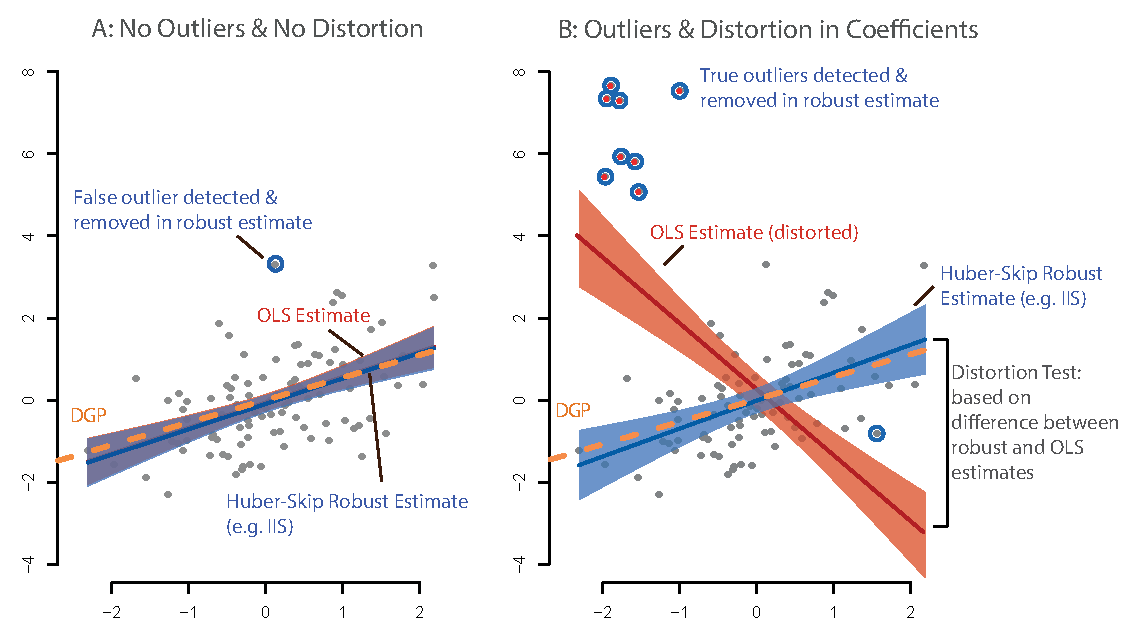
\includegraphics[scale=0.7]{stylized_example_simple_paper_v2.pdf}
\caption{Stylized example of outlier distortion using artificial data. Left panel A shows OLS (red) and robust Huber-skip estimates (blue) when there are no distorting outliers. The DGP is shown as orange-dashed. Right panel B shows 8 outliers distorting the OLS estimates, where the difference between the OLS and robust coefficient estimates is used to construct our proposed distortion test. When no outliers are present, OLS is preferred. When outliers are present and distorting coefficient estimates, the robust estimator is preferred.}
\label{fig_out_styl}
\end{figure}

To establish the proposed outlier distortion test, we need to study the asymptotic behaviour of the RLS/IIS and two step robust procedure in general. Using the empirical process CLT recently developed by \cite{berenguer2019analysis}, we build up an asymptotic theory of this class of robust estimators with an argument similar to \cite{johansen2009analysis, johansen2013outlier, johansen2019boundedness} which study M-estimators. The theory suggests two improvements to the naive two step procedure. First, the ordinary variance estimator needs to be bias-corrected due to the fact that some observations have certain chances to be wrongly classified as outliers and removed under the null of no outliers. Second, to further gain robustness the two step procedure can be iterated until converging to a fixed point which is shown to have the same first order asymptotics as the Huber-skip M-estimator. This paper then establishes tightness, stochastic expansion, and weak convergence of the robust estimators produced by the improved iterated procedure in cross-sectional or time series regressions with stationary, deterministically or stochastically trending regressors. Implementation of RLS/IIS requires selecting a cut-off value, the tuning parameter, to detect outlying observations based on their residuals. The cut-off value as robustification parameter determines the trade-off between robustness and efficiency for the robust estimator RLS/IIS. \cite{jiao2018testing} provides a guidance on choosing this robustification parameter based on an asymptotic study of the false outlier detection rate. The theory derived in this paper holds uniformly for the robustification parameter.

To improve finite sample performance and to alleviate concerns on distributional assumptions on errors, we further introduce and explore three bootstrap testing schemes of our distortion test. First, we non-parametrically re-sample the raw data, which is conservative under the null hypothesis of no outliers and lacks power under alternatives. Second, we re-sample from the outlier-removed clean data. Here we face concerns about size as the cleaned data may appear rather different than the raw data. This is due to the fact that clean data was obtained by targeting a reference distribution. Therefore, we propose a third bootstrap scheme, in which we assess outlier distortion by re-sampling from the clean data but classify outliers at a looser cut-off threshold for bootstrapping samples. The idea being that outliers under a lower cut-off in the clean sample, mimic the relationship of the clean sample to the original raw data. This approach captures some of the characteristics of the data that are not forced to conform to the reference distribution. As expected, all schemes perform reasonably well under the null, however, re-sampling the raw data itself has close to zero power. The re-scaled clean data bootstrap performs best overall with good size and power properties in finite samples, even when the reference distribution is incorrect.

The literature on outlier robustness has not commonly focused on testing presence of distortion. Two papers, however, are notable exceptions and closely related to our approach. First, \cite{kaji2018switching} also asymptotically studies the outlier removal estimator RLS as well as other robust estimators, such as the winsorized estimator, all of which can be represented as L-statistics (integrals of transformations of empirical quantile functions with respect to corresponding random sample selection measures). To establish their asymptotic theory, he then develops a new empirical process theory and a functional delta method for its quantile process tailored for these L-statistics, with an important innovation to the choice of $L_{1}$ norm (instead of the standard $L_{\infty}$ norm in the literature). His argument can be extended to instrumental variables regressions, but requires iid observations. Compared to \cite{kaji2018switching}, we characterise the RLS/IIS and other Huber-skip type estimators as a different type and new class of weighted and marked empirical processes, whose theory has been established by \cite{berenguer2019analysis} via martingale decompositions. Our argument is constructed specially for the RLS/IIS, thus it allows us to dig deeper for these two algorithms. For example, our theory can explore the asymptotics of the variance estimator, iteration of the algorithms, the varying robustification parameter, and the algorithms starting with other initial estimators like least trimmed squares. In addition, our analysis does not require iid data and is also valid for time series regressions with stationary, deterministically trending, and unit root regressors.

To establish the outlier distortion test based on the difference between OLS and RLS estimators, \cite{kaji2018switching} applies the nonparametric bootstrap by randomly sampling the original data with replacement to draw the joint distribution of the outlier removal and the full sample estimators (RLS and OLS). The bootstrap scheme does not require a distributional assumption on the error term, however, it has lower power under a range of alternatives where there are influential outliers distorting regression parameters. This is because when resampling from the original data, the bootstrapping scheme has a certain chance of picking up outliers. Those bootstrapping samples which inlucde outliers will then distort the distribution of the testing statistics and drive it away from what it should be under the null of no outliers.

Second, \cite{dehon2012extending} propose a similar Hausman type test for comparing OLS to the robust S-estimators. Asymptotic theory of the S-estimators has been well established in the robust statistics literature, thus they do not need to derive the asymptotics when constructing the outlier distortion test for the S-estimators. To study the difference between OLS and RLS/IIS, we need to fully establish the theory of RLS/IIS using the empirical process CLT recently developed by \cite{berenguer2019analysis}, although there have been some related work to research M and L type estimators, see \cite{hendry2008automatic}, \cite{johansen2009analysis, johansen2013outlier, johansen2016analysis, johansen2016asymptotic, johansen2019boundedness}, \cite{jiao2015asymptotic}. In addition, \cite{dehon2012extending} restrict their study in the iid setup, whereas time series regressions are allowed in our framework.

In the wider literature on Huber-skip estimators, there is some other closely related work. \cite{jiao2018testing} study whether the proportion (and number) of outliers is different to the expected proportion (and number) when no outliers are present. \cite{jiao2019robustIV} and \cite{jiao2021asymptoitcFODR2SLS} restrict the setup in iid data, and then extend asymptotic theory of the RLS/IIS algorithms and their false outlier detection rate to instrumental variables regressions. \cite{berenguer2018marked} and \cite{berenguer2021heteroscedasticity} considers diagnostic testing on residuals for normality and heteroskedasticity after outlier removal by robust Huber-skip regressions.

We apply our proposed test of outlier distortion to estimate the macro-economic impacts of climate change using the robust IIS estimator. Specifically, we estimate a macro-economic climate impact model in line with the growing panel-econometric literature modelling GDP per capita growth as a function of (non-linear) climate variables. We make two contributions to the existing climate-econometric literature. First, beyond existing estimates, we consider income-based adaptation, allowing the impact of year-on-year changes in temperatures to vary by country-specific income levels. Second, to address un-modelled (and a-priori unknown) idiosyncratic shocks, we apply the robust IIS estimator. We then test for outlier distortion of the estimated coefficients.

Our results firstly show that conventional OLS panel estimates of this relationship are significantly different to those obtained using the robust estimator. Once we control for these outliers (some of which coincide with the first Gulf War and collapse of the Soviet Union), the estimated impacts of temperatures on economic growth are attenuated both for our base model and our adaptation model at all income levels compared to conventional OLS estimates. We secondly find significant evidence of income-driven adaptation to temperatures, where climate effects are dampened as incomes increase, suggesting that richer countries will have a greater capacity to deal with the consequences of continued climate change, in turn exacerbating existing cross-country inequality. Using these estimates and insights, we then compare the effect of the robust estimation and income adaptation in projections of climate impacts to the end of the century under various temperature scenarios.

Projection results consistently indicate that higher levels of warming could lead to higher impacts on GDP per capita with our base model indicating a near two third reduction of median country-level GDP per capita when compared to a baseline and warming beyond 4\textdegree C. Both robust estimation and allowing for income-based adaptation lower these negative impacts, with robust estimation attenuating impacts by up to 10\% and income adaptation by up to 12\% points for high warming scenarios. Robust estimation in this context affects projected impacts mainly at the high and low end of the climate impcat projection distribution.

The paper proceeds as follows: \S \ref{sec_theory and methods} presents our main results with all proofs shown in Appendix \S \ref{sec_proofs}. In particular, \S \ref{sec_algorithm} and \S \ref{sec_assumptions} introduces a regression model, a list of assumptions required for analysis, and a class of outlier-robust algorithms including RLS and IIS. \S \ref{sec_weak convergence} establishes asymptotic theory of RLS and IIS, whilst \S \ref{sec_outlier distortion test} proposes the outlier distortion test. Then, \S \ref{sec_simulations} conducts Monte Carlo studies with additional simulation results in Appendix \S \ref{sec_add_sim}. Lastly, \S \ref{sec_application} applies the outlier distortion test to the macro-economic impacts of climate change using the robust IIS estimator.



\section{Outlier Distortion Test} \label{sec_theory and methods}
We consider a linear regression model
\begin{equation} \label{regression model}
y_{i} = x_{i}^{\prime} \beta + \varepsilon_{i}, \quad i = 1, 2, \ldots, n,
\end{equation}
for the data $\{ (y_{i}, x_{i}) \}_{i = 1}^{n}$, where $y_{i}$ is univariate and $x_{i}$ is multivariate with the dimension $d_{x}$. This setting can represent both classical, time series, and panel regression models. Moreover, in our analysis, regressors $x_{i}$ can be either stationary, deterministically trending, unit root, or explosive processes. Innovations $\varepsilon_{i} / \sigma$ are independent of the filtration $\mathcal{F}_{i-1} = \sigma(x_{1}, \ldots, x_{i}, \varepsilon_{1}, \ldots, \varepsilon_{i-1})$ with the common density $\mathsf{f}$ and distribution function $\mathsf{F}(c) = \mathsf{P}(\varepsilon_{i}/\sigma \le c)$. Denote $\mathsf{g}$ as the density of the absolute error $|\varepsilon_{i}| / \sigma$ and its distribution function by $\mathsf{G}(c) = \mathsf{P}(|\varepsilon_{i}| / \sigma \le c)$ for $c > 0$. Assuming symmetry of $\mathsf{f}$, $\mathsf{G}(c) = 2\mathsf{F}(c) - 1$ and $\mathsf{g}(c) = 2\mathsf{f}(c)$. Define $\psi_{c} = \mathsf{G}(c)$ so the probability of exceeding the cut-off $c$ is $\gamma_{c} = 1 - \psi_{c}$. Suppose the $k$-th moment of the density $\mathsf{f}$ exists, we then define the $k$th moment and truncated moment as
\begin{equation} \label{moments and truncated moments}
\tau_{k} = \int_{- \infty}^{\infty} u^{k} \mathsf{f}(u) du, \qquad \tau_{k}^{c} = \int_{-c}^{c} u^{k} \mathsf{f}(u) du.
\end{equation}
Thus, $\tau_{0}^{c} = \psi_{c}$, $\tau_{2} = 1$ while $\tau_{k} = \tau_{k}^{c} = 0$ for odd $k$ under symmetry. We define the conditional variance of $\varepsilon_{i}/\sigma$ given $( |\varepsilon_{i}|/\sigma \le c )$ as
\begin{equation} \label{bias correction factor}
\varsigma_{c}^{2} = \frac{\tau_{2}^{c}}{\psi_{c}} = \frac{\int_{-c}^{c} u^{2} \mathsf{f}(u) du}{\mathsf{P}(|\varepsilon_{i}| \le \sigma c)}.
\end{equation}
This is the bias correction factor for the variance estimate computed from the selected non-outlying sample. For the Normal reference $\varepsilon_{i} / \sigma \sim \mathsf{N}(0, 1)$, then $\tau_{2}^{c} = \psi_{c} - 2c\mathsf{f}(c)$, $\tau_{4}^{c} = 3 \psi_{c} - 2c(c^{2} + 3)\mathsf{f}(c)$ and $\tau_{4} = 3$.

Outliers are pairs of observations that do not conform with the model (\ref{regression model}) or with the assumed density $\mathsf{f}$. We are interested in the presence of outliers where the errors $\varepsilon_{i} / \sigma$ are drawn from the reference distribution $\mathsf{f}$ but potentially contaminated by an arbitrary (possibly fatter tail) unknown distribution $\mathsf{f}^{\mathrm{c}}$ under $\epsilon$-contamination as in \cite{huber1964robust}
\begin{equation} \label{epsilon contamination}
(1 - \epsilon) \mathsf{f} + \epsilon \mathsf{f}^{\mathrm{c}}.
\end{equation}
This framework allows the data generated by the reference distribution $\mathsf{f}$ to be contaminated by an $\epsilon$ (between 0 and 1) proportion of outliers. Compared to not imposing a parametric distribution on errors, the mixture model of $\mathsf{f}$ and $\mathsf{f}^{\mathrm{c}}$ in (\ref{epsilon contamination}) is an alternative way to relax the assumption on $\varepsilon_{i} / \sigma \sim \mathsf{f}$. The null hypothesis of no outliers in the model (\ref{regression model}) can be formally defined under (\ref{epsilon contamination}) as $H_{0}: \epsilon = 0$ against the alternative $H_{1}: \epsilon > 0$. The following section describes the iterated 1-step Huber-skip M-estimator where we subsequently derive its asymptotic properties and present a new Durbin-Hausman-Wu type test to formalize outlier robustness checks and to assess $H_{0}: \epsilon = 0$.


\subsection{Robust Algorithms to Outliers} \label{sec_algorithm}
There are two potential improvements to the trimmed least squares (the simple two step procedure) used in the empirical literature and the example of \cite{acemoglu2019democracy}. First, \cite{johansen2009analysis} suggest that the updated variance estimator should be corrected by the factor $\varsigma^{-2}$ introduced in (\ref{bias correction factor}), since the simple procedure underestimates $\sigma^{2}$ in the case where observations are identified by chance and falsely removed as outliers. Second, robustness of the estimator could be improved by iterating the 1-step procedure. Considering these two improvements, we introduce and study the so called \emph{iterated 1-step Huber-skip M-estimators} in Algorithm \ref{iterated 1-step Huber-skip M-estimator with the same cut-off c}:

\begin{algorithm} \label{iterated 1-step Huber-skip M-estimator with the same cut-off c}
Choose a cut-off $c > 0$. \\
1. Choose initial estimators $\widehat{\beta}_{c}^{(0)}$, $(\widehat{\sigma}_{c}^{(0)})^{2}$ and let $m = 0$. \\
2. Define indicator variables for selecting non-outlying observations
\begin{equation} \label{iterated 1-step Huber-skip M-indicator with subscript c}
    v_{i, c}^{(m)}
    = 1_{(|y_{i} - x_{i}^{\prime}\widehat{\beta}_{c}^{(m)}|
    \le \widehat{\sigma}_{c}^{(m)} c)}.
\end{equation}
3. Compute least squares estimators
\begin{align}
    \widehat{\beta}_{c}^{(m+1)} &
    = (\sum_{i=1}^{n} x_{i}x_{i}^{\prime} v_{i, c}^{(m)})^{-1}
    (\sum_{i=1}^{n} x_{i}y_{i}  v_{i, c}^{(m)}),
    \label{iterated 1-step Huber-skip M-estimator with subscript c} \\
    (\widehat{\sigma}_{c}^{(m+1)})^{2} &
    = \varsigma_{c}^{-2} (\sum_{i=1}^{n} v_{i, c}^{(m)})^{-1}
    \{ \sum_{i=1}^{n} (y_{i} - x_{i}^{\prime} \widehat{\beta}_{c}^{(m+1)})^{2} v_{i, c}^{(m)} \}.
    \label{iterated regression variance estimator with subscript c}
\end{align}
4. Let $m = m + 1$ and repeat 2 and 3.
\end{algorithm}

Having defined the robust algorithm \ref{iterated 1-step Huber-skip M-estimator with the same cut-off c}, we need to specify initial estimators $\widehat{\beta}_{c}^{(0)}$, $(\widehat{\sigma}_{c}^{(0)})^{2}$. The first initial estimator in our analysis uses the full sample OLS estimates as in \cite{acemoglu2019democracy} and we refer to this as \emph{Robustified Least Squares} (RLS). As a second approach, we use a robust initial estimator and refer to this approach as \emph{Impulse Indicator Saturation} (IIS), described in Algorithm \ref{impulse indicator saturation algorithm}. In IIS we divide the full sample into two sub-samples and use regression estimates calculated from each sub-sample to detect outliers in the other sub-sample:

%To start the Algorithm \ref{iterated 1-step Huber-skip M-estimator with the same cut-off c} with the more robust initial estimator, we could divide the full sample into two sub-samples and use regression estimates calculated from each sub-sample to detect outliers in the other sub-sample. This stylized `split-half' approach is named by \cite{hendry1999econometrics} as the \emph{\textbf{Impulse Indicator Saturation}} (IIS):

% used to derive the theory of IIS (see algorithm \ref{impulse indicator saturation algorithm}), however, as the location of contaminated observations is unknown in most practical situations, the initial sets $\mathcal{I}_{1}$ and $\mathcal{I}_{2}$ should be iterated as is currently implemented in IIS in the R-package \emph{gets} (Pretis et al. 2018) as well as \emph{Autometrics} (Doornik, 2009).

\begin{algorithm} \label{impulse indicator saturation algorithm}
\textbf{Stylized Impulse Indicator Saturation}. Choose a cut-off $c > 0$. \\
1.1. Split full sample into two sets $\mathcal{I}_{j}$, $j = 1, 2$ of $n_{j}$ observations where $\sum_{j=1}^{2} n_{j} = n$. \\
1.2. Calculate least squares estimators based upon each sub-sample $\mathcal{I}_{j}$ for $j = 1, 2$
\begin{equation} \label{IIS initial estimator}
\widehat{\beta}_{j} = (\sum_{i \in \mathcal{I}_{j}} x_{i}x_{i}^{\prime})^{-1} (\sum_{i \in \mathcal{I}_{j}} x_{i}y_{i}), \qquad \widehat{\sigma}_{j}^{2} = \frac{1}{n_{j}} \sum_{i \in \mathcal{I}_{j}} (y_{i} - x_{i}^{\prime} \widehat{\beta}_{j})^{2}.
\end{equation}
1.3. Define the initial indicator variables for selecting non-outlying observations
\begin{equation} \label{IIS initial indicator}
v_{i, c}^{(0)} = 1_{(i \in \mathcal{I}_{1})} 1_{(|y_{i} - x_{i}^{\prime}\widehat{\beta}_{2}| \le \widehat{\sigma}_{2}c)} + 1_{(i \in \mathcal{I}_{2})} 1_{(|y_{i} - x_{i}^{\prime}\widehat{\beta}_{1}| \le \widehat{\sigma}_{1}c)}.
\end{equation}
1.4. Compute $\widehat{\beta}_{c}^{(1)}$, $(\widehat{\sigma}_{c}^{(1)})^{2}$ using $(\ref{iterated 1-step Huber-skip M-estimator with subscript c})$, $(\ref{iterated regression variance estimator with subscript c})$ with $m = 0$, and then let $m = 1$. \\
2. Follow the step 2,3,4 in Algorithm \ref{iterated 1-step Huber-skip M-estimator with the same cut-off c}.
\end{algorithm}


% \subsection{The False Discovery Rate: Gauge} \label{sec_gauge}
% The above outlier detection algorithms RLS and IIS have a positive probability of finding outliers even when, in fact, the data generation process has no outliers. We evaluate the performance of such algorithms by the concept of a gauge, which is the expected retention rate of falsely
% discovered outliers. This is a measure of type I error and it gives us an indirect way of choosing the cut-off $c$. It is defined as follows. The RLS and IIS algorithms assign stochastic indicators $v_{i, c}^{(m)}$ to all observations such that $v_{i, c}^{(m)} = 0$ when observation $i$ is declared as an outlier, otherwise $v_{i, c}^{(m)} = 1$. Given the cut-off $c$ and the iteration $m$ for the Algorithm \ref{iterated 1-step Huber-skip M-estimator with the same cut-off c} (including RLS and IIS), the \textbf{\emph{gauge}} is the proportion of outliers defined under $H_{0}$ as
% \begin{equation} \label{sample and population gauge}
% \widehat{\gamma}_{c}^{(m)} = \frac{1}{n} \sum_{i=1}^{n} (1 - v_{i, c}^{(m)}).
% \end{equation}

The iterated 1-step Huber-skip M-estimator mimics the \cite{huber1964robust} skip\footnote{See \cite{hampel1986robust} (p.\ 104) for the Huber-skip type estimator as opposed to the Huber estimator with the criterion function
\begin{equation*}
\rho (t) =
\begin{cases}
\frac{t^{2}}{2}, & \mbox{if $|t| \le c$}, \\
c |t| - c^{2} / 2, & \mbox{otherwise}.
\end{cases}
\end{equation*}
.} estimator with the criterion function
\begin{equation} \label{Huber-skip criterion}
\rho (t) =
\begin{cases}
\frac{t^{2}}{2}, & \mbox{if $|t| \le c$}, \\
\frac{c^2}{2}, & \mbox{otherwise},
\end{cases}
\end{equation}
which is immune to either outliers or a fatter tail distribution (defined relative to the reference $\mathsf{f}$) under the $\epsilon$-contamination $(1 - \epsilon) \mathsf{f} + \epsilon \mathsf{f}^{\mathrm{c}}$. \cite{johansen2013outlier} argues that Algorithm \ref{iterated 1-step Huber-skip M-estimator with the same cut-off c} is an approximation to and thus an implementation of the Huber-skip regression. \cite{jiao2018testing} provide the guidance for selecting the robustification parameter $c$ and address the testing problem for overall presence of outliers by theoretically analyzing the false discovery rate (referred to as the gauge) of outliers detected by Algorithm \ref{iterated 1-step Huber-skip M-estimator with the same cut-off c}. The main purpose of this paper is to formalize outlier robustness checks using Algorithm \ref{iterated 1-step Huber-skip M-estimator with the same cut-off c} as the Durbin-Hausman-Wu type test by establishing weak convergence of the iterated 1-step Huber-skip M-estimator with the drifting cut-off $c$.


\subsection{Assumptions for Asymptotic Theory} \label{sec_assumptions}
Innovations $\varepsilon_{i}$ and regressors $x_{i}$ must satisfy moment conditions as outlined in Assumption \ref{sufficient assumptions} for our asymptotic analysis. Regressors $x_{i}$ can be temporally dependent and deterministically or stochastically trending. We therefore require a normalisation matrix $N$ that allows for different behaviour of the components of the regressor vector $x_i$. In the case of a stationary regressor we need a standard $n^{-1/2}$ normalisation so that $N$ must be proportional to the identity matrix of the same dimension as $x_i$, that is $N = n^{-1/2}I_{d_{x}}$. Likewise, if $x_i$ is a random walk we have $N = n^{-1}I_{d_{x}}$. Explosive processes are also allowed by our analysis, for example $x_{i} = 2^{i}$ such that the normalization becomes $2^{-n}$. If the regressors are unbalanced as in $x_i=(1, i, 2^{i})'$ we can choose $N=\mathrm{diag} (n^{-1/2}, n^{-3/2}, 2^{-n})$. Thus, denote the normalized regressors as $x_{in} = N^{\prime} x_{i}$.

\begin{assumption} \label{sufficient assumptions}
Let $\mathcal{F}_{i}$ be an increasing sequence of $\sigma$-fields so $\varepsilon_{i-1}$ and $x_{i}$ are $\mathcal{F}_{i-1}$ measurable and $\varepsilon_{i}$ is independent of $\mathcal{F}_{i-1}$. Let $\varepsilon_{i} / \sigma$ have a symmetric, continuously differentiable density $\mathsf{f}$ which is positive on the real line $\mathbb{R}$. For some values of $\eta$ such that $0 < \eta \le 1/4$, choose an integer $r \ge 2$ so
\begin{equation} \label{tradeoff btw moments and boundedness}
2^{r - 1} > 1 + (1/4 - \eta) (1 + d_{x}).
\end{equation}
Let $q = 1 + 2^{r + 1}$. Suppose \\
$(i)$ the density $\mathsf{f}$ satisfies \\
\indent $(a)$ $|u|^{q}\mathsf{f}(u)$, $|u^{q+1}\dot{\mathsf{f}}(u)|$ are decreasing for large $u$; \\
% \indent $(b)$ $\mathsf{f}(u_{n} - n^{-1/4}A)/\mathsf{f}(u_{n}) = \mathrm{O}(1)$ as $n \to \infty$ for some $A > 0$ and all sequences $u_{n} \to \infty$ such that $u_{n} = \mathrm{o}(n^{1/4})$; \\
% \indent $(c)$ $\mathsf{f}(u)/[ u \{1 -\mathsf{F}(u)\} ] = \mathrm{O}(1)$ for $u \to \infty$; \\
$(ii)$ the regressors $x_{i}$ satisfy \\
\indent $(a)$ $\Sigma_{n} = \sum_{i=1}^{n} x_{in} x_{in}^{\prime} \overset{\mathsf{D}}{\to} \Sigma \overset{a.s.}{>} 0$; \\
% \indent $(b)$ $\max_{1 \le i \le n} |n^{1/2 - \kappa} x_{in}| = \mathrm{O}_{\mathsf{P}}(1)$; \\
\indent $(b)$ $n^{-1} \mathsf{E} \sum_{i=1}^{n} |n^{1/2} x_{in}|^{q} = \mathrm{O}(1)$; \\
$(iii)$ the initial estimator $( \widetilde{\beta}, \widetilde{\sigma}^{2} )$ satisfies \\
\indent $(a)$ $N^{-1}(\widetilde{\beta} - \beta) = \mathrm{O}_{\mathsf{P}}(n^{1/4 - \eta})$; \\
\indent $(b)$ $n^{1/2} (\widetilde{\sigma}^{2} - \sigma^{2}) = \mathrm{O}_{\mathsf{P}}(n^{1/4 - \eta})$.
\end{assumption}

While these assumptions may appear abstract, conditions $(i)$, $(ii)$ are satisfied in a range of situations. In particular, the condition $(i)$ is satisfied by the Normal and t distribution; see Remark 2.5 in \cite{berenguer2018marked},
% while the conditions $(ib, ic)$ are satisfied by the Normal distribution, see Johansen and Nielsen (2016b, Remark 2).
while the condition $(ii)$ is satisfied by stationary, random walk and deterministically trending regressors; see Example 3.2 in \cite{johansen2016analysis}, as well as by explosive processes; see Remark 4.2(c) in \cite{berenguer2019analysis}. Condition $(iii)$ allows the standardised estimation errors to diverge at a rate of $n^{1/4 - \eta}$ rather than being bounded in probability. In particular, $\eta = 1/4$ can be chosen for estimators with standard convergence rates.

There is a trade-off in (\ref{tradeoff btw moments and boundedness}) between $\eta$, the divergence rate of initial estimators $\widetilde{\beta}$, $\widetilde{\sigma}^{2}$, and $r$, the required number of moments for innovations $\varepsilon_{i}$ and regressors $x_{i}$. If we have standard initial estimators which are bounded in probability after normalization, such as Robustified Least Squares and Impulse Indicator Saturation, then $\eta$ becomes $1/4$ so we can choose $r = 2$ regardless of dimension of regressors, implying we only require the lower number of moments. Whereas for non-standard diverging estimators, i.e. $0 < \eta < 1/4$ and $1/4 - \eta > 0$, then the required number $r$ of moments grows linearly with the dimension of the regressor. This would be relevant for the $n^{1/3}$-consistent least median of squares regression estimator proposed by \cite{rousseeuw1984least}.


\subsection{Weak Convergence} \label{sec_weak convergence}
%We now provide asymptotic theory for the iterated one-step Huber-skip M-estimator, such as tightness, stochastic expansions, fixed points of the iterated estimators calculated by Algorithm \ref{iterated 1-step Huber-skip M-estimator with the same cut-off c}. The argument holds uniformly in cut-off values. Then, weak convergence is given for Robustified Least Squares and Impulse Indicator Saturation.
To formalise the outlier robustness checks of comparing OLS to robust estimators like RLS/IIS as a statistical test, we need to first fully study asymptotic behaviours of such robust estimators. This paper focuses on a class of iterated one-step Huber-skip estimators, whose analysis requires the empirical process theory recently developed by \cite{berenguer2019analysis}. Therefore, in this section we provide asymptotic theory such as tightness, stochastic expansions, fixed points of the iterated estimators computed by Algorithm \ref{iterated 1-step Huber-skip M-estimator with the same cut-off c} and establish weak convergence of RLS/IIS. Then, equipped with the weak convergence results, the next section is ready to propose our outlier distortion tests. The argument holds uniformly in cut-off values and can extend to developing the outlier distortion tests using other types of robust estimators as long as their limiting distributions are well established.

The first theorem shows that the iterated estimator produced by Algorithm \ref{iterated 1-step Huber-skip M-estimator with the same cut-off c} is tight in the iteration $m \in [0, \infty)$ and in the cut-off value $c \in [c_{+}, \infty)$. Note that $c_{+} > 0$ is a small positive number.

\begin{theorem} \label{tightness of iterated estimators}
Consider the iterated 1-step Huber-skip M-estimator in Algorithm \ref{iterated 1-step Huber-skip M-estimator with the same cut-off c}. Suppose Assumption \ref{sufficient assumptions} holds with $\eta = 1/4$. Then, as $n \to \infty$
\begin{equation*}
\sup_{0 \le m < \infty} \sup_{c_{+} \le c < \infty} |N^{-1} (\widehat{\beta}_{c}^{(m)} - \beta)| + |n^{1/2} (\widehat{\sigma}_{c}^{(m)} - \sigma)| = \mathrm{O}_{\mathsf{P}}(1).
\end{equation*}
\end{theorem}

Firstly, Assumption \ref{sufficient assumptions}$(iii)$ with $\eta = 1/4$ corresponds to a standard convergence rate for the initial estimator. With the 1-step relationship between the updated and the original estimator provided by Lemma \ref{one step expansion of iterated estimators}, also see Corollary \ref{expansion of the first step estimators}, the tightness can then be demonstrated by a geometric argument and mathematical induction.

Firstly, the above tightness theorem implies the uniform consistency of the iterated estimators computed by Algorithm \ref{iterated 1-step Huber-skip M-estimator with the same cut-off c}, that is $\widehat{\beta}_{c}^{(m)} \overset{\mathsf{P}}{\to} \beta$ and $\widehat{\sigma}_{c}^{(m)} \overset{\mathsf{P}}{\to} \sigma$ uniformly in the cut-off value $c$ and iteration step $m$ as $n \to \infty$. Secondly, the tightness will also be used to establish fixed points $\widehat{\beta}_{c}^{(\ast)}$ and $\widehat{\sigma}_{c}^{(\ast)}$ of Algorithm \ref{iterated 1-step Huber-skip M-estimator with the same cut-off c} upon through infinite iterations when $m \to \infty$ and to demonstrate weak convergence theory of RLS and IIS.

The next theorem is to show stochastic expansions of any iterated step estimators of Algorithm \ref{iterated 1-step Huber-skip M-estimator with the same cut-off c} in terms of the initial estimators, kernels, and small remainder terms.

\begin{theorem} \label{general expansion in terms of initial estimators}
Consider the iterated 1-step Huber-skip M-estimator in Algorithm \ref{iterated 1-step Huber-skip M-estimator with the same cut-off c}. Suppose Assumption \ref{sufficient assumptions} holds with $\eta = 1/4$. Then, as $n \to \infty$ and uniformly in $c \in [c_{+}, \infty)$, we have for any $m \in [0, \infty)$
\begin{align*}
N^{-1} (\widehat{\beta}_{c}^{(m + 1)} - \beta) & = \varrho_{\beta, c}^{(m + 1)} N^{-1} (\widehat{\beta}_{c}^{(0)} - \beta) + \varrho_{x \varepsilon, c}^{(m + 1)} \Sigma_{n}^{-1} \sum_{i = 1}^{n} x_{in} \varepsilon_{i} 1_{(|\varepsilon_{i}| \le \sigma c)} +  \mathrm{o}_{\mathsf{P}}(1), \\
n^{1/2} (\widehat{\sigma}_{c}^{(m + 1)} - \sigma) & = \varrho_{\sigma, c}^{(m + 1)} n^{1/2} (\widehat{\sigma}_{c}^{(0)} - \sigma) + \varrho_{\varepsilon \varepsilon, c}^{(m + 1)} n^{-1/2} \sum_{i=1}^{n} (\frac{\varepsilon_{i}^{2}}{\sigma^{2}} - \varsigma_{c}^{2}) 1_{(|\varepsilon_{i}| \le \sigma c)} +  \mathrm{o}_{\mathsf{P}}(1),
\end{align*}
where coefficients have expressions
\begin{align*}
\varrho_{\beta, c}^{(m + 1)} & = \{ \frac{2 c \mathsf{f}(c)}{\psi_{c}} \}^{m + 1},  & \varrho_{x \varepsilon, c}^{(m + 1)} & = \frac{\psi_{c}^{m + 1} - \{ 2 c \mathsf{f}(c) \}^{m + 1}}{\psi_{c}^{m + 1} \{ \psi_{c} - 2 c \mathsf{f}(c) \}}, \\
\varrho_{\sigma, c}^{(m + 1)} & = \{ \frac{c (c^{2} - \varsigma_{c}^{2}) \mathsf{f}(c)}{\tau_{2}^{c}} \}^{m + 1} , & \varrho_{\varepsilon \varepsilon, c}^{(m + 1)} & = \sigma \frac{(\tau_{2}^{c})^{m + 1} - \{ c (c^{2} - \varsigma_{c}^{2}) \mathsf{f}(c) \}^{m + 1}}{2 (\tau_{2}^{c})^{m + 1} \{ \tau_{2}^{c} - c (c^{2} - \varsigma_{c}^{2}) \mathsf{f}(c) \}}.
\end{align*}
\end{theorem}

The above theorem generalises Lemma \ref{one step expansion of iterated estimators} in the sense that its proof is to recursively apply the one-step expansion of the updated estimator in terms of the original ones. Let $m = 0$ such that $\varrho_{\beta, c}^{(1)} = 2 c \mathsf{f}(c) / \psi_{c}$, $\varrho_{x \varepsilon, c}^{(1)}  = \psi_{c}^{-1}$, $\varrho_{\sigma, c}^{(1)} = c (c^{2} - \varsigma_{c}^{2}) \mathsf{f}(c) / \tau_{2}^{c}$, and $\varrho_{\varepsilon \varepsilon, c}^{(1)} = \sigma / (2 \tau_{2}^{c})$, then the expansion immediately reduces to the one-step case. Here, we provide the following corollary to re-express Lemma \ref{one step expansion of iterated estimators} as a stochastic expansion of the fist step estimators in terms of the initial ones and the kernel terms.

\begin{corollary} \label{expansion of the first step estimators}
Consider the iterated 1-step Huber-skip M-estimator in Algorithm \ref{iterated 1-step Huber-skip M-estimator with the same cut-off c}. Suppose Assumption \ref{sufficient assumptions} holds with $\eta = 1/4$. Then, as $n \to \infty$ and uniformly in $c \in [c_{+}, \infty)$, we have
\begin{align*}
N^{-1} (\widehat{\beta}_{c}^{(1)} - \beta) & = \frac{2 c \mathsf{f}(c)}{\psi_{c}} N^{-1} (\widehat{\beta}_{c}^{(0)} - \beta) +  (\psi_{c} \Sigma_{n})^{-1} \sum_{i = 1}^{n} x_{in} \varepsilon_{i} 1_{(|\varepsilon_{i}| \le \sigma c)} +  \mathrm{o}_{\mathsf{P}}(1), \\
n^{1/2} (\widehat{\sigma}_{c}^{(1)} - \sigma) & = \frac{c (c^{2} - \varsigma_{c}^{2}) \mathsf{f}(c)}{\tau_{2}^{c}} n^{1/2} (\widehat{\sigma}_{c}^{(0)} - \sigma) \\
& + \frac{\sigma}{2 \tau_{2}^{c}} n^{-1/2} \sum_{i=1}^{n} (\frac{\varepsilon_{i}^{2}}{\sigma^{2}} - \varsigma_{c}^{2}) 1_{(|\varepsilon_{i}| \le \sigma c)} +  \mathrm{o}_{\mathsf{P}}(1).
\end{align*}
\end{corollary}

Initially the tight estimator is assumed to be available and it is subsequently iterated through the above one-step expansion. Assumption \ref{sufficient assumptions}$(i)$ implies that autoregressive coefficients $2c \mathsf{f}(c)/\psi_{c}$ and $c(c^{2} - \varsigma_{c}^{2})\mathsf{f}(c)/\tau_{2}^{c}$ are strictly bounded by one holding uniformly in $c$, suggesting that the above equation is a contraction mapping. Thus, Algorithm \ref{iterated 1-step Huber-skip M-estimator with the same cut-off c} will converge to a fixed point as the iteration step increases to be sufficiently large. Let $m \to \infty$ in Theorem \ref{general expansion in terms of initial estimators} such that $\varrho_{\beta, c}^{(\infty)} = 0$, $\varrho_{x \varepsilon, c}^{(\infty)} = 1 / \{ \psi_{c} - 2 c \mathsf{f}(c) \}$, $\varrho_{\sigma, c}^{(\infty)} = 0$, and $\varrho_{\varepsilon \varepsilon, c}^{(\infty)} = \sigma / [ 2 \{ \tau_{2}^{c} - c (c^{2} - \varsigma_{c}^{2}) \mathsf{f}(c) \} ]$, then the below theorem finds the fixed point $N^{-1} (\widehat{\beta}_{c}^{(\ast)} - \beta) = N^{-1} (\widehat{\beta}_{c}^{(\infty)} - \beta)$, $n^{1/2} (\widehat{\sigma}_{c}^{(\ast)} - \sigma) = n^{1/2} (\widehat{\sigma}_{c}^{(\infty)} - \sigma)$.

\begin{theorem} \label{fixed point of iterated estimators}
Consider the iterated 1-step Huber-skip M-estimator in Algorithm \ref{iterated 1-step Huber-skip M-estimator with the same cut-off c}. Suppose Assumption \ref{sufficient assumptions} holds with $\eta = 1/4$. Then, for all $\epsilon, \delta > 0$ a pair $m_{0}, n_{0} > 0$ exists, so for all $m > m_{0}$ and $n > n_{0}$
\begin{equation*}
\mathsf{P} \{ \sup_{c_{+} \le c < \infty} | N^{-1}(\widehat{\beta}_{c}^{(m)} - \widehat{\beta}_{c}^{(\ast)}) | + | n^{1/2}(\widehat{\sigma}_{c}^{(m)} - \widehat{\sigma}_{c}^{(\ast)}) | > \delta \} < \epsilon,
\end{equation*}
where
\begin{align*}
N^{-1}(\widehat{\beta}_{c}^{(\ast)} - \beta) & = \frac{1}{\psi_{c} - 2c\mathsf{f}(c)} \Sigma_{n}^{-1} \sum_{i=1}^{n} x_{in} \varepsilon_{i} 1_{(|\varepsilon_{i}| \le \sigma c)}, \\
n^{1/2}(\widehat{\sigma}_{c}^{(\ast)} - \sigma) & = \frac{\sigma}{2 \{ \tau_{2}^{c} - c(c^{2} - \varsigma_{c}^{2})\mathsf{f}(c) \}} n^{-1/2}  \sum_{i=1}^{n} (\frac{\varepsilon_{i}^{2}}{\sigma^{2}} - \varsigma_{c}^{2}) 1_{(|\varepsilon_{i}| \le \sigma c)}.
\end{align*}
\end{theorem}

The proof is conducted as follows. According to Theorem \ref{tightness of iterated estimators}, if the initial estimator is bounded in a large compact set with a large probability, then any iterated estimators of Algorithm \ref{iterated 1-step Huber-skip M-estimator with the same cut-off c} take values in the same compact set no matter what value of the cut-off $c$ is chosen. Next, the argument is to further demonstrate that the deviation between the $m$-fold iterated estimator and the fixed point is the sum of two terms vanishing exponentially and in probability respectively as $m$ and $n$ go to infinity.

Theorem \ref{fixed point of iterated estimators} shows the first order asymptotics of the fixed point of Algorithm \ref{iterated 1-step Huber-skip M-estimator with the same cut-off c} and it is in fact the same as that of the \cite{huber1964robust} skip estimator, thus the iterated one-step Huber-skip M-estimator mimics the Huber-skip estimator and Algorithm \ref{iterated 1-step Huber-skip M-estimator with the same cut-off c} can be understood as an implementation of the Huber-skip estimation as a non-linear optimisation problem.

The choice of the initial estimator does not affect Algorithm \ref{iterated 1-step Huber-skip M-estimator with the same cut-off c} in terms of finding the fixed point, as long as it has the tightness property. Thus, the fixed point theorem also applies for RLS and IIS as well as the theorems regarding to tightness and stochastic expansions, since the full sample or split sample least squares as their starting estimators are tight. Next concentrating on RLS and IIS, we first show their stochastic expansions in order to establish weak convergence theory.

\begin{theorem} \label{general expansion for RLS and IIS}
Consider Robustified Least Squares (RLS) or split half Impulse Indicator Saturation where $n_{1} = \mathrm{int}[n / 2]$ and $n_{2} = n - n_{1}$ (IIS). Suppose Assumption \ref{sufficient assumptions}$(i, ii)$ holds for each sub-sample set $\mathcal{I}_{1}$, $\mathcal{I}_{2}$.
Then, as $n \to \infty$ and uniformly in $c \in [c_{+}, \infty)$ we have for any $m \in [0, \infty)$
\begin{align*}
N^{-1} (\widehat{\beta}_{c}^{(m + 1)} - \beta) & = \varrho_{\beta, c}^{(m + 1)} \Sigma_{n}^{-1} \sum_{i = 1}^{n} x_{in} \varepsilon_{i} + \varrho_{x \varepsilon, c}^{(m + 1)} \Sigma_{n}^{-1} \sum_{i = 1}^{n} x_{in} \varepsilon_{i} 1_{(|\varepsilon_{i}| \le \sigma c)} +  \mathrm{o}_{\mathsf{P}}(1), \\
n^{1/2} (\widehat{\sigma}_{c}^{(m + 1)} - \sigma) & = \varrho_{\sigma, c}^{(m + 1)} \frac{\sigma}{2} n^{-1/2} \sum_{i = 1}^{n} (\frac{\varepsilon_{i}^{2}}{\sigma^{2}} - 1) \\
& + \varrho_{\varepsilon \varepsilon, c}^{(m + 1)} n^{-1/2} \sum_{i=1}^{n} (\frac{\varepsilon_{i}^{2}}{\sigma^{2}} - \varsigma_{c}^{2}) 1_{(|\varepsilon_{i}| \le \sigma c)} +  \mathrm{o}_{\mathsf{P}}(1),
\end{align*}
where the coefficients $\varrho_{\beta, c}^{(m + 1)}, \varrho_{x \varepsilon, c}^{(m + 1)}, \varrho_{\sigma, c}^{(m + 1)}, \varrho_{\varepsilon \varepsilon, c}^{(m + 1)}$ are defined in Theorem \ref{general expansion in terms of initial estimators}.
\end{theorem}

Substituting the expansion of the full sample least squares as the initial estimator in Theorem \ref{general expansion in terms of initial estimators}, we immediately prove the above theorem for RLS. Then, we find that the split half version of IIS has the identical expansion as RLS. The first step updated estimator and the fixed point of RLS and IIS are two special cases of our main interest, so their expansions can be obtained by letting $m = 0$ and $m \to \infty$. With Theorem \ref{general expansion for RLS and IIS}, we are now ready to establish the weak convergence theory for RLS and IIS in cases where the regressors are either stationary, deterministic trend, or unit root processes.

Theorem \ref{tightness of iterated estimators} demonstrates uniform consistency of the iterated estimators of $\beta, \sigma^{2}$. In this paper, we are concerned about whether the $\beta$ coefficient is distorted due to outliers. Thus, the next step is to focus on distributional analysis of the iterated estimator of $\beta$. Thus, using the stochastic expansion of the $\beta$ estimator in Theorem \ref{general expansion for RLS and IIS}, it suffices to analyse the distribution of the kernel vector $\sum_{i = 1}^{n} (x_{in}^{\prime} \varepsilon_{i}, x_{in}^{\prime} \varepsilon_{i} 1_{(|\varepsilon_{i}| \le \sigma c)})^{\prime}$. With this purpose in mind, we need to first discuss in a few situations the choice of the normalisation matrix $N$ in $x_{in} = N^{\prime} x_{i}$ and the limiting behaviour of the covariance matrix of the normalised regressors $\Sigma_{n} = \sum_{i = 1}^{n} x_{in} x_{in}^{\prime}$.

\emph{Stationary case}. Suppose the regressors are cross-sectional iid or arise from a stationary time series model. Thus, we choose $N = n^{-1/2} I_{d_{x}}$ for normalising the regressors such that $x_{in} = N^{\prime} x_{i} = n^{-1/2} x_{i}$. Then, $\Sigma_{n} = \sum_{i = 1}^{n} x_{in} x_{in}^{\prime} = n^{-1} \sum_{i = 1}^{n} x_{i} x_{i}^{\prime}$ converges in probability to a deterministic term $\Sigma = \mathsf{E} x_{i} x_{i}^{\prime}$ by LLN. To investigate the asymptotic behaviour of the kernel vector, we apply martingale CLT so that for any $c \in [c_{+}, \infty)$
\begin{equation*}
\sum_{i = 1}^{n}
\begin{pmatrix}
x_{in} \varepsilon_{i} \\
x_{in} \varepsilon_{i} 1_{(|\varepsilon_{i}| \le \sigma c)}
\end{pmatrix}
=
n^{-1/2} \sum_{i = 1}^{n}
\begin{pmatrix}
x_{i} \varepsilon_{i} \\
x_{i} \varepsilon_{i} 1_{(|\varepsilon_{i}| \le \sigma c)}
\end{pmatrix}
\overset{\mathsf{D}}{\to}
\mathsf{N}
\begin{Bmatrix}
\begin{pmatrix}
0_{d_{x}} \\
0_{d_{x}}
\end{pmatrix}
,
\sigma^{2} \tau_{2}^{c}
\begin{pmatrix}
\frac{1}{\tau_{2}^{c}} \Sigma & \Sigma \\
\Sigma & \Sigma
\end{pmatrix}
\end{Bmatrix}
.
\end{equation*}

Drifting cut-off values $c$ in the interval $[c_{+}, \infty)$, we obtain a sequence of processes $\mathbb{G}_{n}^{(m + 1)}(c) = N^{-1} (\widehat{\beta}_{c}^{(m + 1)} - \beta) = n^{1/2} (\widehat{\beta}_{c}^{(m + 1)} - \beta)$ for any $m \in [0, \infty)$. We can now establish a weak convergence theory for $\mathbb{G}_{n}^{(m + 1)}$, which follows from a finite dimensional convergence and tightness; see \cite{billingsley1968convergence}. The below theorem then shows that RLS and IIS are asymptotically approximated by a Gaussian process.

\begin{theorem} \label{weak convergence for RLS and IIS}
Consider RLS or IIS. Suppose Assumption \ref{sufficient assumptions}$(i, ii)$ holds. For any $m \in [0, \infty)$, denote the processes $\mathbb{G}_{n}^{(m + 1)}(c) = n^{1/2} (\widehat{\beta}_{c}^{(m + 1)} - \beta)$ with the argument $c \in [c_{+}, \infty)$. Then as $n \to \infty$, $\mathbb{G}_{n}^{(m + 1)}$ weakly converges to a zero mean Gaussian process $\mathbb{G}^{(m + 1)}$ with variance
\begin{equation*}
\mathsf{Var} \{ \mathbb{G}^{(m + 1)}(c) \} = \{ (\varrho_{\beta, c}^{(m + 1)})^{2} + 2 \tau_{2}^{c} \varrho_{\beta, c}^{(m + 1)} \varrho_{x \varepsilon, c}^{(m + 1)} + \tau_{2}^{c} (\varrho_{x \varepsilon, c}^{(m + 1)})^{2} \} \sigma^{2} \Sigma^{-1},
\end{equation*}
where $\varrho_{\beta, c}^{(m + 1)}$, $\varrho_{x \varepsilon, c}^{(m + 1)}$ are defined in Theorem \ref{general expansion in terms of initial estimators}.
\end{theorem}

Again, the one-step updated estimator and fixed point are of particular interest in RLS or IIS. To explore their weak convergence, let $m = 0$ and $m \to \infty$ in Theorem \ref{weak convergence for RLS and IIS} such that $\varrho_{\beta, c}^{(1)} = 2 c \mathsf{f}(c) / \psi_{c}$, $\varrho_{x \varepsilon, c}^{(1)} = \psi_{c}^{-1}$ and $\varrho_{\beta, c}^{(\infty)} = 0$, $\varrho_{x \varepsilon, c}^{(\infty)} = 1 / \{ \psi_{c} - 2 c \mathsf{f}(c) \}$, then we have the below corollary.

\begin{corollary} \label{weak convergence for the first step and fixed point of RLS and IIS}
Consider RLS or IIS. Suppose Assumption \ref{sufficient assumptions}$(i, ii)$ holds. The cut-off $c$ drifts in the interval $[c_{+}, \infty)$. Then as $n \to \infty$, for $m = 0$ a sequence of processes $\mathbb{G}_{n}^{(1)}$ of the initial estimator weakly converges to a zero mean Gaussian process $\mathbb{G}^{(1)}$ with variance
\begin{equation*}
\mathsf{Var} \{ \mathbb{G}^{(1)}(c) \} = \frac{4 c^{2} \mathsf{f}^{2}(c) + 4 \tau_{2}^{c} c \mathsf{f}(c) + \tau_{2}^{c}}{\psi_{c}^{2}} \sigma^{2} \Sigma^{-1}.
\end{equation*}
In addition, for $m \to \infty$ a sequence of processes $\mathbb{G}_{n}^{(\ast)}$ of the fixed point estimator weakly converges to a zero mean Gaussian process $\mathbb{G}^{(\ast)}$ with variance
\begin{equation*}
\mathsf{Var} \{ \mathbb{G}^{(\ast)}(c) \} = \frac{\tau_{2}^{c}}{\{ \psi_{c} - 2 c \mathsf{f}(c) \}^{2}} \sigma^{2} \Sigma^{-1}.
\end{equation*}
\end{corollary}

\emph{Deterministic trends}. To keep notations simple and analysis clear, here we consider a straightforward example which follows the regression
\begin{equation*}
y_{i} = \beta_{0} + \beta_{1} i + \varepsilon_{i}, \quad i = 1, 2, \ldots, n.
\end{equation*}
For the regressors $x_{i} = (1, i)^{\prime}$, we choose the normalisation matrix
$
N =
\begin{pmatrix}
n^{-1/2} & 0 \\
0 & n^{-3/2}
\end{pmatrix}
$ so that $x_{in} = N^{\prime} x_{i} = (n^{-1/2}, n^{-3/2} i)^{\prime}$. Then, it follows
\begin{equation*}
\Sigma_{n} = \sum_{i = 1}^{n} x_{in} x_{in}^{\prime} =
\sum_{i = 1}^{n}
\begin{pmatrix}
n^{-1} & n^{-2} i \\
n^{-2} i & n^{-3} i^{2}
\end{pmatrix}
\to
\begin{pmatrix}
1 & 1/2 \\
1/2 & 1/3
\end{pmatrix}
= \Sigma.
\end{equation*}
Notice that we use $\sum_{i = 1}^{n} i = n (n + 1) / 2$ and $\sum_{i = 1}^{n} i^{2} = n (n + 1) (2n + 1) / 6$ to obtain the above deterministic limit. The kernel vector $\sum_{i = 1}^{n} (x_{in}^{\prime} \varepsilon_{i}, x_{in}^{\prime} \varepsilon_{i} 1_{(|\varepsilon_{i}| \le \sigma c)})^{\prime}$ has a limiting normal distribution with the same form of mean and variance as given in the stationary case where instead $d_{x} = 2$ and $\Sigma$ is derived immediately above. For any $m \in [0, \infty)$, denote a sequence of processes of the iterated estimators computed by RLS or IIS as
$
\mathbb{G}_{n}^{(m + 1)}(c) = N^{-1} (\widehat{\beta}_{c}^{(m + 1)} - \beta) =
\begin{Bmatrix}
n^{1/2} (\widehat{\beta}_{0, c}^{(m + 1)} - \beta_{0}) \\
n^{3/2} (\widehat{\beta}_{1, c}^{(m + 1)} - \beta_{1})
\end{Bmatrix}
$
with $c \in [c_{+}, \infty)$. Thus as $n \to \infty$, $\mathbb{G}_{n}^{(m + 1)}$ weakly converges to a zero mean Gaussian process with the same form of variance as given in Theorem \ref{weak convergence for RLS and IIS} and Corollary \ref{weak convergence for the first step and fixed point of RLS and IIS} where again $\Sigma$ needs to be changed to the one shown above.

Other cases of deterministic trends can be studied using a similar analysis to the above example. For instance, the argument applies to trend stationary autoregressions but involves a notationally tedious detrending derivation; see Section 1.5.1 in \cite{johansen2009analysis} for a related and more detailed description.

\emph{Unit roots}. Consider the I(1) process, which follows the autoregression
\begin{equation*}
y_{i} = \beta y_{i - 1} + \varepsilon_{i}, \quad i = 1, 2, \ldots, n,
\end{equation*}
where $\beta = 1$. Other cases of unit roots processes can be analysed similarly using the following argument. Firstly, we choose $N = n^{-1}$ for normalising the regressor $x_{i} = y_{i - 1}$ so that $x_{in} = N^{\prime} x_{i} = n^{-1} y_{i - 1} = n^{-1} y_{0} + n^{-1} \sum_{s = 1}^{i - 1} \varepsilon_{s}$. For any $c \in [c_{+}, \infty)$ and as $n \to \infty$, the functional CLT shows that a sequence of processes
$
n^{-1/2} \sum_{s = 1}^{\mathrm{int}(nu)}
\begin{pmatrix}
\varepsilon_{s} \\
\varepsilon_{s} 1_{(|\varepsilon_{s}| \le \sigma c)}
\end{pmatrix}
$
weakly converges to a Brownian motion
$
\begin{pmatrix}
B_{1, u} \\
B_{2, u}
\end{pmatrix}
$ with the argument $u \in [0, 1]$ having the mean zero and variance
$
\sigma^{2}
\begin{pmatrix}
1 & \tau_{2}^{c} \\
\tau_{2}^{c} & \tau_{2}^{c}
\end{pmatrix}
$.
Next, we find
\begin{equation*}
\Sigma_{n} = \sum_{i = 1}^{n} x_{in} x_{in}^{\prime} = n^{-2} \sum_{i = 1}^{n} y_{i - 1}^{2} = n^{-1} \sum_{i = 1}^{n} (n^{-1/2} \sum_{s = 1}^{i - 1} \varepsilon_{s} + n^{-1/2} y_{0})^{2} \overset{\mathsf{D}}{\to} \int_{0}^{1} B_{1, u}^{2} du = \Sigma.
\end{equation*}
For any $c \in [c_{+}, \infty)$, the kernel vector then follows
\begin{equation*}
\sum_{i = 1}^{n}
\begin{pmatrix}
x_{in} \varepsilon_{i} \\
x_{in} \varepsilon_{i} 1_{(|\varepsilon_{i}| \le \sigma c)}
\end{pmatrix}
=
n^{-1/2} \sum_{i = 1}^{n}
\begin{pmatrix}
n^{-1/2} y_{i - 1} \varepsilon_{i} \\
n^{-1/2} y_{i - 1}  \varepsilon_{i} 1_{(|\varepsilon_{i}| \le \sigma c)}
\end{pmatrix}
\overset{\mathsf{D}}{\to}
\begin{pmatrix}
\int_{0}^{1} B_{1, u} d B_{1, u} \\
\int_{0}^{1} B_{1, u} d B_{2, u}
\end{pmatrix}
.
\end{equation*}
Theorem \ref{general expansion for RLS and IIS} shows that
\begin{equation*}
N^{-1} (\widehat{\beta}_{c}^{(m + 1)} - \beta) =
\begin{pmatrix}
\varrho_{\beta, c}^{(m + 1)} \Sigma_{n}^{-1} \\
\varrho_{x \varepsilon, c}^{(m + 1)} \Sigma_{n}^{-1}
\end{pmatrix}^{\prime}
\sum_{i = 1}^{n}
\begin{pmatrix}
x_{in} \varepsilon_{i} \\
x_{in} \varepsilon_{i} 1_{(|\varepsilon_{i}| \le \sigma c)}
\end{pmatrix}
+ \mathrm{o}_{\mathsf{P}}(1).
\end{equation*}
With the above results, we can now establish the limiting distribution of the iterated estimator produced by RLS or IIS for any cut-off value so that for any $m \in [0, \infty)$ and $c \in [c_{+}, \infty)$ it follows as $n \to \infty$ that
\begin{equation*}
n (\widehat{\beta}_{c}^{(m + 1)} - \beta) \overset{\mathsf{D}}{\to} \frac{\varrho_{\beta, c}^{(m + 1)} \int_{0}^{1} B_{1, u} dB_{1, u} + \varrho_{x \varepsilon, c}^{(m + 1)} \int_{0}^{1} B_{1, u} dB_{2, u}}{\int_{0}^{1} B_{1, u}^{2} du}.
\end{equation*}
Remember from Theorem \ref{general expansion in terms of initial estimators} that
\begin{equation*}
\varrho_{\beta, c}^{(m + 1)} = \{ \frac{2 c \mathsf{f}(c)}{\psi_{c}} \}^{m + 1},  \qquad \varrho_{x \varepsilon, c}^{(m + 1)} = \frac{\psi_{c}^{m + 1} - \{ 2 c \mathsf{f}(c) \}^{m + 1}}{\psi_{c}^{m + 1} \{ \psi_{c} - 2 c \mathsf{f}(c) \}}.
\end{equation*}

Once again, special interests lie in the first step and fixed point estimators of RLS and IIS. Thus, let $m = 0$ and $m \to \infty$ in the above limiting distribution such that $\varrho_{\beta, c}^{(1)} = 2 c \mathsf{f}(c) / \psi_{c}$, $\varrho_{x \varepsilon, c}^{(1)} = \psi_{c}^{-1}$ and $\varrho_{\beta, c}^{(\infty)} = 0$, $\varrho_{x \varepsilon, c}^{(\infty)} = 1 / \{ \psi_{c} - 2 c \mathsf{f}(c) \}$, then for any $c \in [c_{+}, \infty)$ it follows as $n \to \infty$ that
\begin{align*}
n (\widehat{\beta}_{c}^{(1)} - \beta) & \overset{\mathsf{D}}{\to} \frac{2 c \mathsf{f}(c) \int_{0}^{1} B_{1, u} dB_{1, u} +  \int_{0}^{1} B_{1, u} dB_{2, u}}{\psi_{c}  \int_{0}^{1} B_{1, u}^{2} du}, \\
n (\widehat{\beta}_{c}^{(\ast)} - \beta) & \overset{\mathsf{D}}{\to} \frac{\int_{0}^{1} B_{1, u} dB_{2, u}}{\{ \psi_{c} - 2 c \mathsf{f}(c) \} \int_{0}^{1} B_{1, u}^{2} du}.
\end{align*}

When $c \to \infty$ then $\psi_{c} \to 1$, $\tau_{2}^{c} \to 1$, and $c \mathsf{f}(c) \to 0$ such that $\varrho_{\beta, c}^{(m + 1)} \to 0$ and $\varrho_{x \varepsilon, c}^{(m + 1)} \to 1$ for any $m \in [0, \infty)$ due to Assumption \ref{sufficient assumptions}$(i)$. Furthermore, two Brownian motions $B_{1}$ and $B_{2}$ become identical, since $1_{(|\varepsilon_{s}| \le \sigma c)} \to 1$ and their variances
$
\sigma^{2}
\begin{pmatrix}
1 & \tau_{2}^{c} \\
\tau_{2}^{c} & \tau_{2}^{c}
\end{pmatrix}
\to
\sigma^{2}
\begin{pmatrix}
1 & 1 \\
1 & 1
\end{pmatrix}
$.
Thus, the limiting distribution of the iterated estimators
\begin{equation*}
\frac{\varrho_{\beta, c}^{(m + 1)} \int_{0}^{1} B_{1, u} dB_{1, u} + \varrho_{x \varepsilon, c}^{(m + 1)} \int_{0}^{1} B_{1, u} dB_{2, u}}{\int_{0}^{1} B_{1, u}^{2} du}
\to
\frac{\int_{0}^{1} B_{1, u} dB_{1, u}}{\int_{0}^{1} B_{1, u}^{2} du},
\end{equation*}
which is the usual Dicky-Fuller distribution. This is not surprising, since for any $m \in [0, \infty)$ and as $c \to \infty$ the iterated estimator $n (\widehat{\beta}_{c}^{(m + 1)} - \beta)$ computed by RLS or IIS becomes the ordinary least squares $n (\widetilde{\beta} - \beta)$ which then converges to the Dicky-Fuller distribution as $n \to \infty$.

With the above weak convergence results of RLS and IIS, the next step is to construct tests for coefficients distortion due to outliers. The proposed tests formalise the common practice for outlier robustness checks by looking into the difference between RLS (or IIS) and OLS.


\subsection{Testing Methods} \label{sec_outlier distortion test}
A frequent concern in empirical economics is whether a tiny set of outliers may have invalidated empirical results. The common practice is to carry out robustness checks by redoing the analyses with the sample after trimming all outliers detected by Algorithm \ref{iterated 1-step Huber-skip M-estimator with the same cut-off c} and comparing results from the original ones with the full sample. Instead of heuristically checking the difference between the trimmed LS and OLS without knowing whether it is statistically significant, this paper formalizes the outlier robustness check as a new type of \cite{durbin1954errors}-\cite{hausman1978specification}-\cite{wu1973alternative} test.

The test is based on trade-off between robustness and efficiency and enables to judge whether the least squares estimation is appropriate or the robust method should be preferred. The robust estimator produced by Algorithm \ref{iterated 1-step Huber-skip M-estimator with the same cut-off c} is consistent both under the null and alternatives (although less efficient under the null\footnote{The trimmed LS would throw away observations wrongly classified as outliers and thus has the higher asymptotic variance than OLS under the null; See the weak convergence result of RLS and IIS in \S \ref{sec_weak convergence}; Also see the discussion in \cite{johansen2009analysis} on the relative efficiency factor (efficiency loss) of IIS.}), whereas OLS is efficient (and consistent) under the null, but inconsistent otherwise. The test statistics is looking on statistically significant difference between RLS/IIS and OLS. If the model is correctly specified, the Hausman type test statistics should be rather small under the null of no outliers, since two consistent methods should produce estimates that are very close to the population. On the contrary when outliers have large influence on least squares estimation, the robust method should be very different from the ordinary estimate, so OLS should be rejected and the RLS/IIS should be preferred. The proposed test thus will evaluate whether the gain in robustness is more valuable than the corresponding loss in efficiency.

In practice, empirical researchers run the full sample OLS $\widetilde{\beta}$ and compare to the trimmed LS $\widehat{\beta}_{c}^{(m + 1)}$. Our proposed test can detect whether two estimates are significantly distinct by exploring on the L2 norm of the difference between $\widetilde{\beta}$ and $\widehat{\beta}_{c}^{(m + 1)}$. Thus, for any $m \in [0, \infty)$ it is essential first to derive the stochastic expansion and weak limit of a sequence of stochastic processes $\mathbb{H}_{n}^{(m + 1)}(c) =N^{-1} (\widehat{\beta}_{c}^{(m + 1)} - \widetilde{\beta})$ with the argument $c \in [c_{+}, \infty)$. We concentrate on stationary regressors in this section, where $N = n^{-1/2} I_{d_{x}}$ such that $\mathbb{H}_{n}^{(m + 1)}(c) =n^{1/2} (\widehat{\beta}_{c}^{(m + 1)} - \widetilde{\beta})$, $x_{in} = n^{-1/2} x_{i}$, and $\Sigma = \mathsf{E} x_{i} x_{i}^{\prime}$. With the weak convergence results shown in \S \ref{sec_weak convergence}, other cases such as deterministic trends and unit roots can be analysed using the same argument.

\begin{theorem} \label{expansion and weak limit of processes of Hausman statistics}
Consider RLS or IIS. Suppose Assumption \ref{sufficient assumptions}$(i, ii)$ holds. For any $m \in [0, \infty)$, denote the processes $\mathbb{H}_{n}^{(m + 1)}(c) = n^{1/2} (\widehat{\beta}_{c}^{(m + 1)} - \widetilde{\beta})$ with the argument $c \in [c_{+}, \infty)$. Then as $n \to \infty$, we have
\begin{equation*}
\mathbb{H}_{n}^{(m + 1)}(c) = (\varrho_{\beta, c}^{(m + 1)} - 1) \Sigma_{n}^{-1} \sum_{i = 1}^{n} x_{in} \varepsilon_{i} + \varrho_{x \varepsilon, c}^{(m + 1)} \Sigma_{n}^{-1} \sum_{i = 1}^{n} x_{in} \varepsilon_{i} 1_{(|\varepsilon_{i}| \le \sigma c)} + \mathrm{o}_{\mathsf{P}}(1),
\end{equation*}
where $\varrho_{\beta, c}^{(m + 1)}$, $\varrho_{x \varepsilon, c}^{(m + 1)}$ are defined in Theorem \ref{general expansion in terms of initial estimators}. Furthermore, $\mathbb{H}_{n}^{(m + 1)}$ weakly converges to a zero mean Gaussian process $\mathbb{H}^{(m + 1)}$ with variance given as
\begin{equation*}
\mathsf{Var} \{ \mathbb{H}^{(m + 1)}(c) \} = \{ (\varrho_{\beta, c}^{(m + 1)} - 1)^{2} + 2 \tau_{2}^{c} (\varrho_{\beta, c}^{(m + 1)} - 1) \varrho_{x \varepsilon, c}^{(m + 1)} + \tau_{2}^{c} (\varrho_{x \varepsilon, c}^{(m + 1)})^{2} \} \sigma^{2} \Sigma^{-1}.
\end{equation*}
\end{theorem}

The proof immediately follows from the stochastic expansion and weak convergence of $\widehat{\beta}_{c}^{(m + 1)}$ in Theorem \ref{general expansion for RLS and IIS} and \ref{weak convergence for RLS and IIS}. Using the weak convergence result of $\mathbb{H}_{n}^{(m + 1)}$, we next establish the outlier distortion test.

\begin{corollary} \label{pointwise convergence of Hausman test statistics}
Consider RLS or IIS. Suppose Assumption \ref{sufficient assumptions}$(i, ii)$ holds. For any $m \in [0, \infty)$, $c \in [c_{+}, \infty)$ and as $n \to \infty$, we have
\begin{equation*}
n^{1/2} (\widehat{\beta}_{c}^{(m + 1)} - \widetilde{\beta}) \overset{\mathsf{D}}{\to} \mathsf{N}\{ 0_{d_{x}}, \mathsf{avar}(\widehat{\beta}_{c}^{(m + 1)} - \widetilde{\beta}) \},
\end{equation*}
where $\mathsf{avar}(\widehat{\beta}_{c}^{(m + 1)} - \widetilde{\beta}) = \{ (\varrho_{\beta, c}^{(m + 1)} - 1)^{2} + 2 \tau_{2}^{c} (\varrho_{\beta, c}^{(m + 1)} - 1) \varrho_{x \varepsilon, c}^{(m + 1)} + \tau_{2}^{c} (\varrho_{x \varepsilon, c}^{(m + 1)})^{2} \} \sigma^{2} \Sigma^{-1}$. Then, the proposed test statistics has the weak limit
\begin{equation*}
H_{n, c}^{(m + 1)} = n (\widehat{\beta}_{c}^{(m + 1)} - \widetilde{\beta})^{\prime} \mathsf{avar}(\widehat{\beta}_{c}^{(m + 1)} - \widetilde{\beta})^{-1} (\widehat{\beta}_{c}^{(m + 1)} - \widetilde{\beta}) \overset{\mathsf{D}}{\to} \chi^{2}_{d_{x}}.
\end{equation*}
\end{corollary}

When two estimators are correlated: one (RLS/IIS $\widehat{\beta}_{c}^{(m + 1)}$) is always consistent but inefficient under the null (of no outliers), the other (OLS $\widetilde{\beta}$) efficient but not consistent under alternatives, then the asymptotic variance of their difference is given by the difference of their respective asymptotic variances under the null. Using the similar argument to \cite{hausman1978specification}, Lemma \ref{equality for asymptotic variance of difference} in the appendix demonstrates the above statement in our context. In addition, we provide a different but more direct proof in Remark \ref{asymptotic variance of difference equals the difference of respective variances} to show $\mathsf{avar}(\widehat{\beta}_{c}^{(m + 1)} - \widetilde{\beta}) = \mathsf{avar}(\widehat{\beta}_{c}^{(m + 1)}) - \mathsf{avar}(\widetilde{\beta})$ under the null of no outliers. It makes use of the asymptotics derived for $\widehat{\beta}_{c}^{(m + 1)}$ in \S \ref{sec_weak convergence} and indicates that the regularity conditions required by Lemma \ref{equality for asymptotic variance of difference} hold for $\mathsf{f} \overset{\mathsf{D}}{=} \mathsf{N}(0, 1)$.

To guarantee the power performance of the outlier distortion test under alternatives, our first recommendation is to use $\mathsf{avar}(\widehat{\beta}_{c}^{(m + 1)} - \widetilde{\beta})$ as suggested in Corollary \ref{pointwise convergence of Hausman test statistics} rather than $\mathsf{avar}(\widehat{\beta}_{c}^{(m + 1)}) - \mathsf{avar}(\widetilde{\beta})$ when constructing the test statistics. It is because although two are equal under the null of no outliers, this would not be the case under alternatives. Furthermore, we need to estimate $\mathsf{avar}(\widehat{\beta}_{c}^{(m + 1)} - \widetilde{\beta})$ in order to conduct the test. Given the chosen iteration step $m$, the cut-off value $c$, and the reference distribution $\mathsf{f}$, the terms $\tau_{2}^{c}$, $\varrho_{\beta, c}^{(m + 1)}$, $\varrho_{x \varepsilon, c}^{(m + 1)}$ appearing in $\mathsf{avar}(\widehat{\beta}_{c}^{(m + 1)} - \widetilde{\beta})$ are known, so parameters that need to be estimated are $\sigma^{2}$, $\Sigma$. Their estimators should be consistent under the null and robust under alternatives, thus our second recommendation is of estimating $\sigma^{2}$, $\Sigma$ using the clean data with all outliers removed, since the full sample estimators are inconsistent under alternatives though efficient under the null. Given any chosen $m \in [0, \infty)$ and $c \in [c_{+}, \infty)$, we can consistently estimate $\sigma^{2}$ and $\Sigma = \mathsf{E} x_{i} x_{i}^{\prime}$ under the null using the subsample of all non-outlying observations by
\begin{align*}
(\widehat{\sigma}_{c}^{(m+1)})^{2} & = \varsigma_{c}^{-2} (\sum_{i=1}^{n} v_{i, c}^{(m)})^{-1} \{ \sum_{i=1}^{n} (y_{i} - x_{i}^{\prime} \widehat{\beta}_{c}^{(m+1)})^{2} v_{i, c}^{(m)} \}, \\
\widehat{\Sigma}_{c}^{(m + 1)} & = (\sum_{i = 1}^{n} v_{i, c}^{(m)})^{-1} (\sum_{i = 1}^{n} x_{i} x_{i}^{\prime} v_{i, c}^{(m)}).
\end{align*}
Thus, our suggested estimator of $\mathsf{avar}(\widehat{\beta}_{c}^{(m + 1)} - \widetilde{\beta})$ is given by
\begin{align}
& \quad \,\, \widehat{\mathsf{avar}}(\widehat{\beta}_{c}^{(m + 1)} - \widetilde{\beta}) \nonumber \\
& = \{ (\varrho_{\beta, c}^{(m + 1)} - 1)^{2} + 2 \tau_{2}^{c} (\varrho_{\beta, c}^{(m + 1)} - 1) \varrho_{x \varepsilon, c}^{(m + 1)} + \tau_{2}^{c} (\varrho_{x \varepsilon, c}^{(m + 1)})^{2} \} (\widehat{\sigma}_{c}^{(m + 1)})^{2} (\widehat{\Sigma}_{c}^{(m + 1)})^{-1}. \label{estimated asymptotic variance}
\end{align}
Otherwise if we use $\mathsf{avar}(\widehat{\beta}_{c}^{(m + 1)}) - \mathsf{avar}(\widetilde{\beta})$ to construct the testing statistics and estimate $\sigma^{2}$ and $\Sigma$ in $\mathsf{avar}(\widetilde{\beta})$ using the full sample, then under alternatives the test would lose power and lead to incorrect results. More seriously, it is very likely under alternatives to have $\widehat{\mathsf{avar}}(\widehat{\beta}_{c}^{(m + 1)})  \le \widehat{\mathsf{avar}}(\widetilde{\beta})$ such that $\widehat{\mathsf{avar}}(\widehat{\beta}_{c}^{(m + 1)}) -\widehat{\mathsf{avar}}(\widetilde{\beta}) \le 0$, thus the Hausman type testing statistics is negative so that the test is meaningless in this case.

We can now fully establish the outlier distortion test for formalising the robustness checks. For any chosen $m \in [0, \infty)$ and $c \in [c_{+}, \infty)$, we have the testing statistics and its limiting distribution
\begin{equation*}
n^{1/2} (\widehat{\beta}_{c}^{(m + 1)} - \widetilde{\beta}) \overset{a}{\sim} \mathsf{N}\{ 0_{d_{x}}, \widehat{\mathsf{avar}}(\widehat{\beta}_{c}^{(m + 1)} - \widetilde{\beta}) \},
\end{equation*}
and
\begin{equation*}
\widehat{H}_{n, c}^{(m + 1)} = n (\widehat{\beta}_{c}^{(m + 1)} - \widetilde{\beta})^{\prime} \widehat{\mathsf{avar}}(\widehat{\beta}_{c}^{(m + 1)} - \widetilde{\beta})^{-1} (\widehat{\beta}_{c}^{(m + 1)} - \widetilde{\beta}) \overset{a}{\sim} \chi^{2}_{d_{x}}.
\end{equation*}
Note that $\widehat{\mathsf{avar}}(\widehat{\beta}_{c}^{(m + 1)} - \widetilde{\beta})$ shown in (\ref{estimated asymptotic variance}) is invertible and its inverse is given by
\begin{align*}
& \quad \,\, \widehat{\mathsf{avar}}(\widehat{\beta}_{c}^{(m + 1)} - \widetilde{\beta})^{-1} \\
& = \{ (\varrho_{\beta, c}^{(m + 1)} - 1)^{2} + 2 \tau_{2}^{c} (\varrho_{\beta, c}^{(m + 1)} - 1) \varrho_{x \varepsilon, c}^{(m + 1)} + \tau_{2}^{c} (\varrho_{x \varepsilon, c}^{(m + 1)})^{2} \}^{-1} (\widehat{\sigma}_{c}^{(m + 1)})^{-2} \widehat{\Sigma}_{c}^{(m + 1)},
\end{align*}
since $(\varrho_{\beta, c}^{(m + 1)} - 1)^{2} + 2 \tau_{2}^{c} (\varrho_{\beta, c}^{(m + 1)} - 1) \varrho_{x \varepsilon, c}^{(m + 1)} + \tau_{2}^{c} (\varrho_{x \varepsilon, c}^{(m + 1)})^{2} \neq 0$. We therefore avoid the rank deficiency problem described and addressed by the generalised inverse in \cite{hausman1981generalized} and \cite{holly1982remark}. The proposed test can either be performed as the two-sided test with the normal limit or as the one-sided test with the chi-squared limit. On implementing RLS or IIS, we are particularly interested in two specific estimators: the trimmed estimator just updated from the full sample OLS and the fixed point estimator iterated upon through infinite steps. The below corollary then provides the outlier distortion tests for these two special cases, checking whether $\widetilde{\beta}$ is distinct from $\widehat{\beta}_{c}^{(1)}$ when $m = 0$ or from $\widehat{\beta}_{c}^{(\ast)}$ when $m \to \infty$.

\begin{corollary} \label{Hausman test when m = 1 and m = infinite}
Consider RLS or IIS. Suppose Assumption \ref{sufficient assumptions}$(i, ii)$ holds. For any $c \in [c_{+}, \infty)$ and large $n$, then when $m = 0$ we have
\begin{equation*}
n^{1/2} (\widehat{\beta}_{c}^{(1)} - \widetilde{\beta}) \overset{a}{\sim} \mathsf{N}\{ 0_{d_{x}}, \widehat{\mathsf{avar}}(\widehat{\beta}_{c}^{(1)} - \widetilde{\beta}) \},
\end{equation*}
and
\begin{equation*}
\widehat{H}_{n, c}^{(1)} = n (\widehat{\beta}_{c}^{(1)} - \widetilde{\beta})^{\prime} \widehat{\mathsf{avar}}(\widehat{\beta}_{c}^{(1)} - \widetilde{\beta})^{-1} (\widehat{\beta}_{c}^{(1)} - \widetilde{\beta}) \overset{a}{\sim} \chi^{2}_{d_{x}},
\end{equation*}
where
\begin{equation*}
\widehat{\mathsf{avar}}(\widehat{\beta}_{c}^{(1)} - \widetilde{\beta}) = \frac{\{2 c \mathsf{f}(c) - \psi_{c} \}^{2} + 2 \tau_{2}^{c} \{2 c \mathsf{f}(c) - \psi_{c} \} + \tau_{2}^{c}}{\psi_{c}^{2}} (\widehat{\sigma}_{c}^{(1)})^{2} (\widehat{\Sigma}_{c}^{(1)})^{-1}.
\end{equation*}
In addition, when $m \to \infty$ we have
\begin{equation*}
n^{1/2} (\widehat{\beta}_{c}^{(\ast)} - \widetilde{\beta}) \overset{a}{\sim} \mathsf{N}\{ 0_{d_{x}}, \widehat{\mathsf{avar}}(\widehat{\beta}_{c}^{(\ast)} - \widetilde{\beta}) \},
\end{equation*}
and
\begin{equation*}
\widehat{H}_{n, c}^{(\ast)} = n (\widehat{\beta}_{c}^{(\ast)} - \widetilde{\beta})^{\prime} \widehat{\mathsf{avar}}(\widehat{\beta}_{c}^{(\ast)} - \widetilde{\beta})^{-1} (\widehat{\beta}_{c}^{(\ast)} - \widetilde{\beta}) \overset{a}{\sim} \chi^{2}_{d_{x}},
\end{equation*}
where
\begin{equation*}
\widehat{\mathsf{avar}}(\widehat{\beta}_{c}^{(\ast)} - \widetilde{\beta}) = \frac{ \{ 2 c \mathsf{f}(c) - \psi_{c} \}^{2} + 2 \tau_{2}^{c} \{ 2 c \mathsf{f}(c) - \psi_{c} \} + \tau_{2}^{c} }{\{ 2 c \mathsf{f}(c) - \psi_{c} \}^{2}} (\widehat{\sigma}_{c}^{(\ast)})^{2} (\widehat{\Sigma}_{c}^{(\ast)})^{-1}.\footnote{If assume $\mathsf{f} \overset{\mathsf{D}}{=} \mathsf{N}(0, 1)$, then $\tau_{2}^{c} = \psi_{c} - 2 c \mathsf{f}(c)$ so that $\widehat{\mathsf{avar}}(\widehat{\beta}_{c}^{(1)} - \widetilde{\beta})$ and $\widehat{\mathsf{avar}}(\widehat{\beta}_{c}^{(\ast)} - \widetilde{\beta})$ can be further simplified.}
\end{equation*}
\end{corollary}

% In the case that the estimated asymptotic variance has deficient rank so that it is not inversible in the Hausman test statistics, Hausman and Taylor (1981) and Holly (1982) suggested using some pseudo-inverse\footnote{Suppose $A$ is a $k \times i$ matrix. If $k \neq i$ or $k = i$ but $A$ has deficient rank, then $A$ is not inversible so $A^{-1}$ does not exist. A Moore-Penrose generalised inverse (pseudo-inverse) $A^{+}$ of $A$ is an $i \times k$ matrix, which is uniquely determined by the following three conditions: \\
% $(i)$ $A A^{+} A = A$; \\
% $(ii)$ $A^{+} A A^{+} = A^{+}$; \\
% $(iii)$ $A A^{+}$ and $A^{+} A$ are symmetric. \\
% If $A$ has full column rank $i$, then $A^{+} = (A^{\prime} A)^{-1} A^{\prime}$.} instead to solve the singularity problem. However, it is clear to check from (\ref{estimated asymptotic variance}) that the inverse of $\widehat{\mathsf{avar}}(\widehat{\beta}_{c}^{(m + 1)} - \widetilde{\beta})$ does exist in our context. Thus, the proposed test avoid applying Moore-Penrose generalized inverse.

\emph{Heuristic tests}. Without the asymptotic theory, some empirical researchers simply use the similar form of the proposed testing statistics but incorrectly replace the standard error of the difference between two estimators $\widetilde{\beta}$ and $\widehat{\beta}_{c}^{(m + 1)}$ by the standard error of the marginal distribution of the baseline estimator $\widetilde{\beta}$. They subsequently compare it with the critical value either drawn from the standard normal for the two-sided test or from the chi-square with $d_{x}$ degree of freedom for the one-sided test. The above procedure is referred to as the heuristic method for the outlier robustness checks. Since the heuristic method is constructed in a mistaken way, its size does not converge to the nominal level under the null and it has a low statistical power under alternatives. Thus, even the heuristic method is informative for preliminary analysis, it is not consistent in theory and not reliable in practice.

Notice that the density $\mathsf{f}$ of the errors $\varepsilon_{i}$ enters in the asymptotic variance of the difference between RLS/IIS and OLS, thus our proposed test needs to assume its distributional form. It is a regularity condition in the outlier detection literature and follows from the $\epsilon$-contamination idea initially proposed by \cite{huber1964robust} and recently re-investigated by \cite{johansen2016analysis}. Under the Huber's framework, data come from $(1 - \epsilon) \mathsf{f} + \epsilon \mathsf{f}^{\mathrm{c}}$, so $\epsilon$ proportion of outliers, generated by an arbitrary (possibly fatter tailed) contaminated distribution $\mathsf{f}^{\mathrm{c}}$, have to be defined relative to a reference distribution $\mathsf{f}$ for $1 - \epsilon$ proportion of sample. Furthermore, many empirical studies implicitly assume a form of the density $\mathsf{f}$ to select the cut-off value $c$ for conducting outlier robustness checks. For example, \cite{acemoglu2019democracy} choose $c = 1.96$ by implicitly imposing the standard normal for the density $\mathsf{f}$ to compute the RLS estimator when assessing the impact of democratisation on economic growth.\footnote{In addition, other IIS and climate applications mentioned in the introduction (from wages to hurricane damages) all implicitly assume a normal reference distribution of the error term.} Thus, the distributional assumption on $\mathsf{f}$ is not necessarily restrictive in our context, and it can be testable by a specification test proposed by \cite{berenguer2018marked} and \cite{jiao2018testing}.

Unlike the proposed asymptotic test, the heuristic test does not depend on the form of $\mathsf{f}$. This is because it wrongly replaces the asymptotic variance of the difference between RLS/IIS and OLS by the asymptotic variance of OLS. Thus, it is meaningless to apply this inconsistent test except for preliminary analysis just to obtain an informative result. For our testing problem, we next move down the bootstrap route to research whether it is possible to robustify the distributional assumption on $\mathsf{f}$.

\emph{Bootstrap tests}. Despite the parametric distribution of the error term being a common assumption, to alleviate concerns about performance under an incorrect reference distribution and to improve finite sample performance, we propose and investigate three bootstrap versions of the outlier distortion test. This paper focuses on a non-parametric bootstrap of the $L_{1}$ and $L_{2}$ norms of the difference between OLS and RLS/IIS.

First, the same as \cite{kaji2018switching}, we investigate the standard non-parametric bootstrap by randomly sampling observations $i$ from the data $\{(y_{i}, x_{i})\}_{i = 1}^{n}$ with replacement to draw the distribution of the $L_{1}$ norm of the difference between $\widehat{\beta}_{c}^{(m + 1)}$ and $\widetilde{\beta}$. Unlike the asymptotic test proposed in this paper, the bootstrap does not require assuming the known form of the density $\mathsf{f}$, but it likely suffers from low power under alternatives where the data is in fact contaminated. This is because under alternatives the bootstrap has a certain probability to sample outlying observations which would have large influence on $\beta$ estimation. For these bootstrapping iterations having sampled large outliers from the original data, the testing statistics on difference between $\widehat{\beta}_{c}^{(m + 1)}$ and $\widetilde{\beta}$ would become rather large, so its bootstrapping distribution would be highly distorted and significantly distinct from what it should be under the null.

Second, we consider re-sampling from the outlier-removed (`cleaned') data. While this approach likely exhibits better power properties, there is a concern that it may be over-sized, as outliers are determined relative to the specified reference distribution, thus forcing the `clean' data to appear closer to the reference distribution even under the null of no outlier distortion.

We therefore propose a third bootstrap approach where we scale the cut-off used to determine outlying observations. We first identify outlying observations at a cut-off $c$ in the raw data, and subsequently re-sample from the cleaned data and create a bootstrap sample of our test statistic (or RLS/IIS) by using $c'$ where $c' < c$. In other words, while the target reference distribution forces the cleaned data to be closer to the assumed distribution, by then relaxing the cut-off, some of the properties of the underlying data will likely be regained. The idea being that outliers identified using a lower threshold $c'$ on the clean data, mimics the removal of outliers from the raw data at $c$.

We study the performance of the three bootstrap schemes together with the proposed asymptotic type test using a range of simulations.



%\vspace{0.5cm}
\section{Finite Sample Performance using Simulations} \label{sec_simulations}
Here we study the performance of the proposed outlier distortion test in a series of simulation experiments under the null hypothesis of no distortion, as well as under a range of alternatives. We simulate (\ref{regression model}) varying the sample size $n$, the number of regressors tested $d_x$, the degree of persistence in the dependent variable (ranging from iid to stochastically-trending), as well as the underlying reference distribution, and the degree of outlier contamination under a range of alternatives (the proportion of outliers as well as outlier magnitude). Simulations are implemented using the R-package  \texttt{gets}, with $m=10,000$ replications for asymptotic tests and $m=1,000$ replications and bootstrap draws for the bootstrap versions of the test.

\subsection{Simulation Performance under the Null of No Distortion}

%We simulate the performance of the distortion test with the estimated models matching the DGP where we vary the number of covariates on which we test for coefficient distortion at varying sample sizes and varying degrees of persistence in the dependent variable, ranging from iid to stochastically-trending.

Simulation results under the null of no outliers are shown in Figure \ref{fig_out_sim_null}. The asymptotic test appears slightly over-sized for small samples ($n<200$) but exhibits size close to the nominal level in larger samples ($n>200$). Size appears unaffected by the threshold used to detect outliers (left panel in \ref{fig_out_sim_null}), the number of coefficients tested for distortion (middle panel in Figure \ref{fig_out_sim_null}), or the degree of persistence of the dependent variable even if $y$ follows a stochastic trend (right panel in Figure \ref{fig_out_sim_null}).

\begin{figure}[!htbp]  %\vspace{-.35in}
\centering
%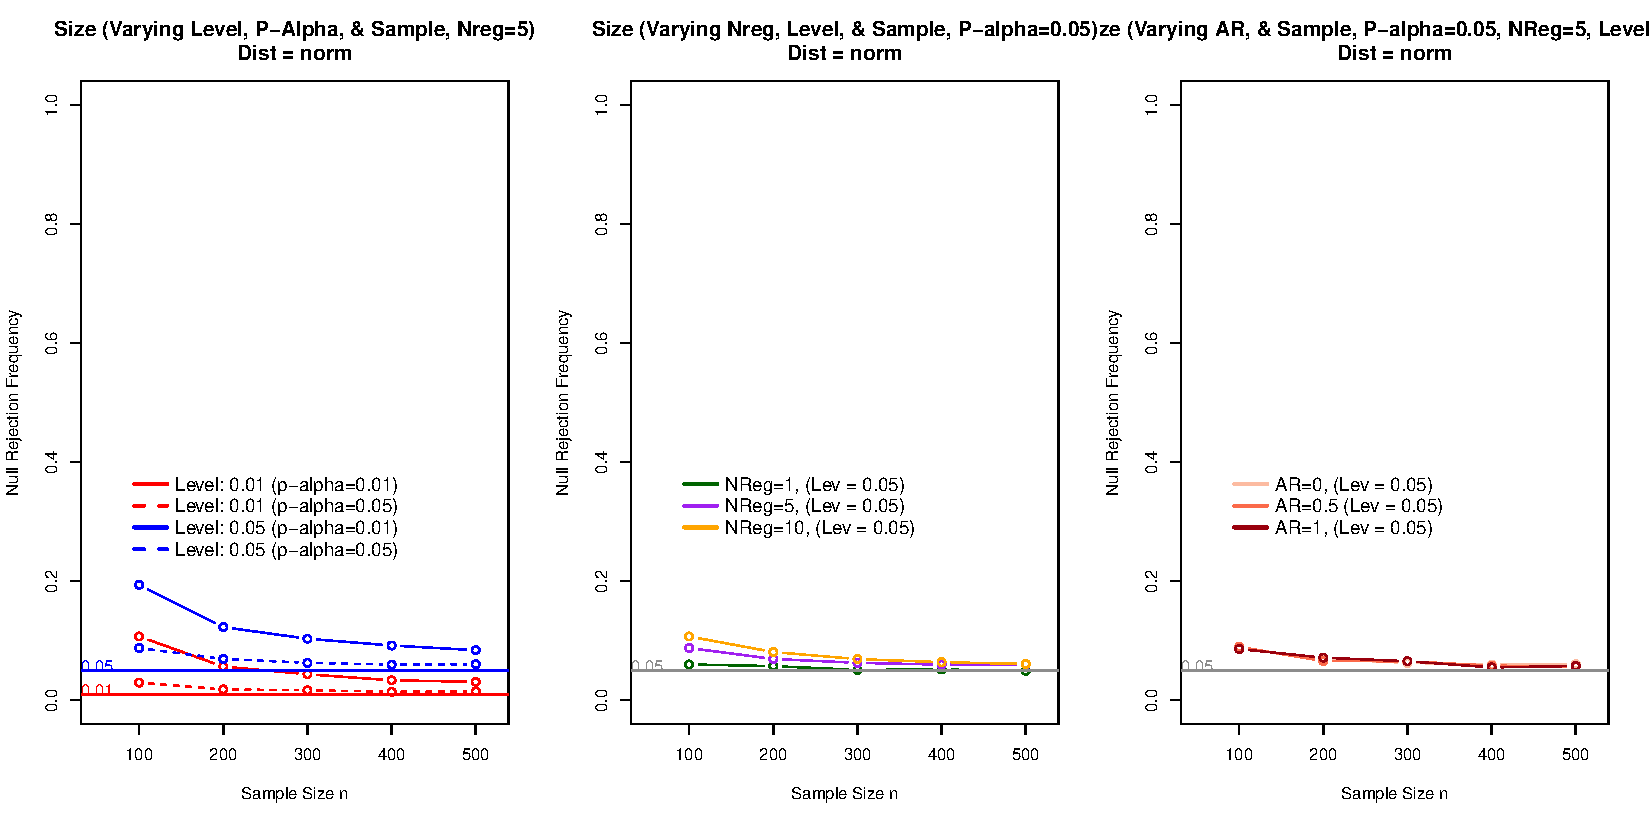
\includegraphics[scale=0.6]{null_distnorm.pdf}
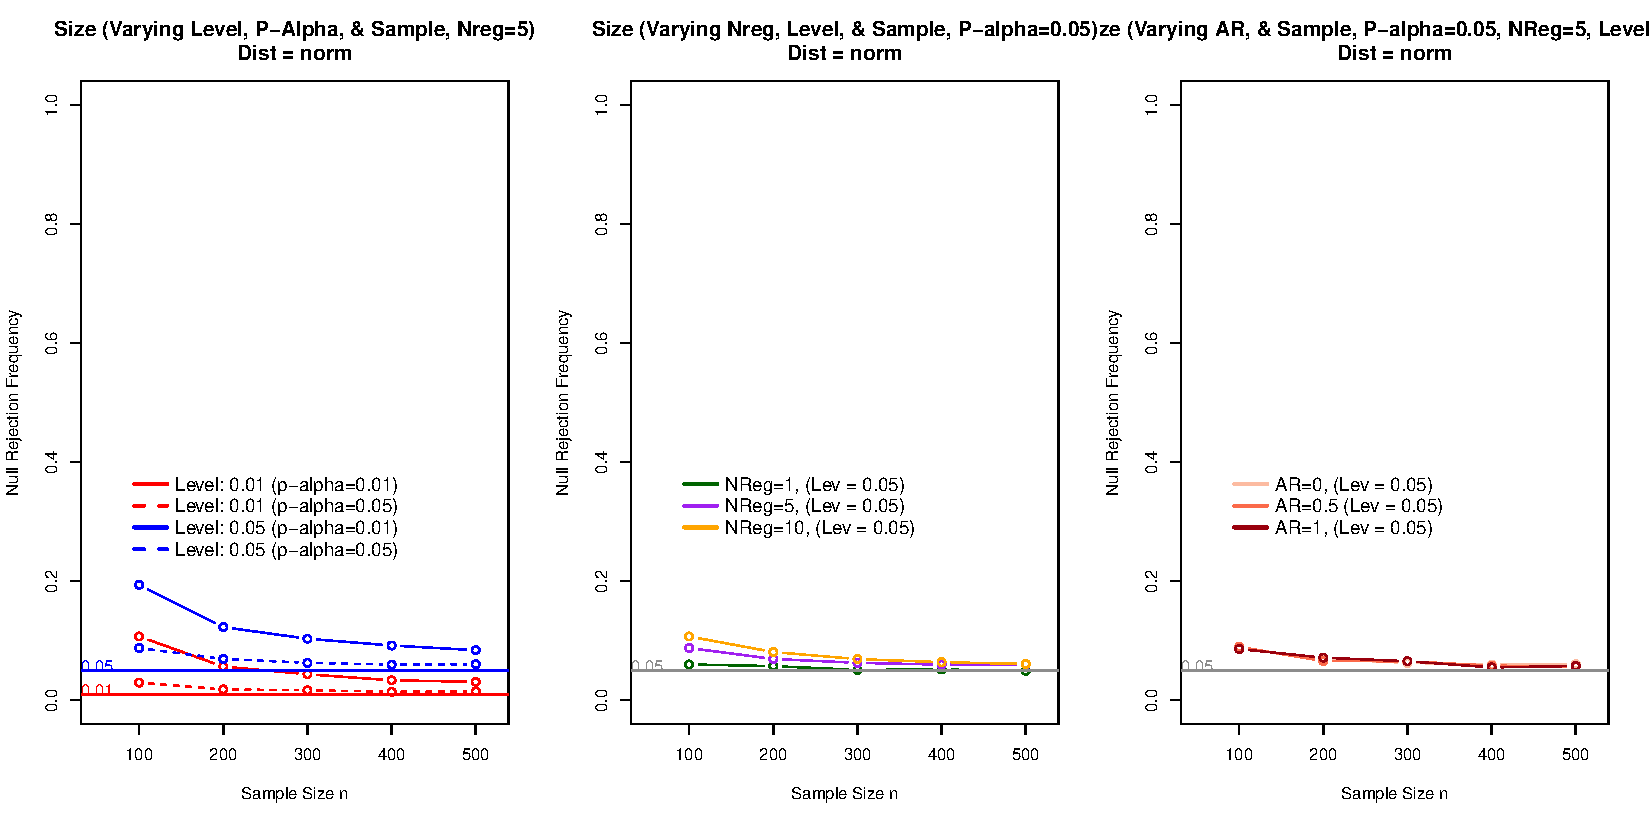
\includegraphics[width = \textwidth]{null_distnorm.pdf}
\caption{Simulation performance of the asymptotic test under the null of no distortion.}
\label{fig_out_sim_null}
\end{figure}

%We investigate the performance of the asymptotic and bootstrap tests

Bootstrap results are shown in Figure \ref{fig_boot_sim_null} using both the $L_{1}$ and $L_{2}$ norm of the difference between robust and OLS coefficient estimates. Here we also consider the performance of the bootstrap and asymptotic tests when the assumed reference distribution is incorrect. Specifically, we consider the case where we assume $\mathsf{f}$ to be a normal reference distribution, when the actual error distribution is fatter-tailed (a $t$-distribution with 3 degrees of freedom).

As expected, the bootstrap on the raw data is under-sized regardless of the reference distribution. In turn, the asymptotic test is over-sized when reference distribution is incorrect. Bootstrapping the clean (outlier-removed) data yields a size close to nominal levels for small samples (under a correct reference distribution), and also partly reduces the over-rejection when the reference distribution is incorrect. Our proposed bootstrap scaling approach improves the performance relative to the asymptotic test when the assumed reference distribution is to the true error distribution.


\begin{figure}[!htbp]  %\vspace{-.35in}
\centering
%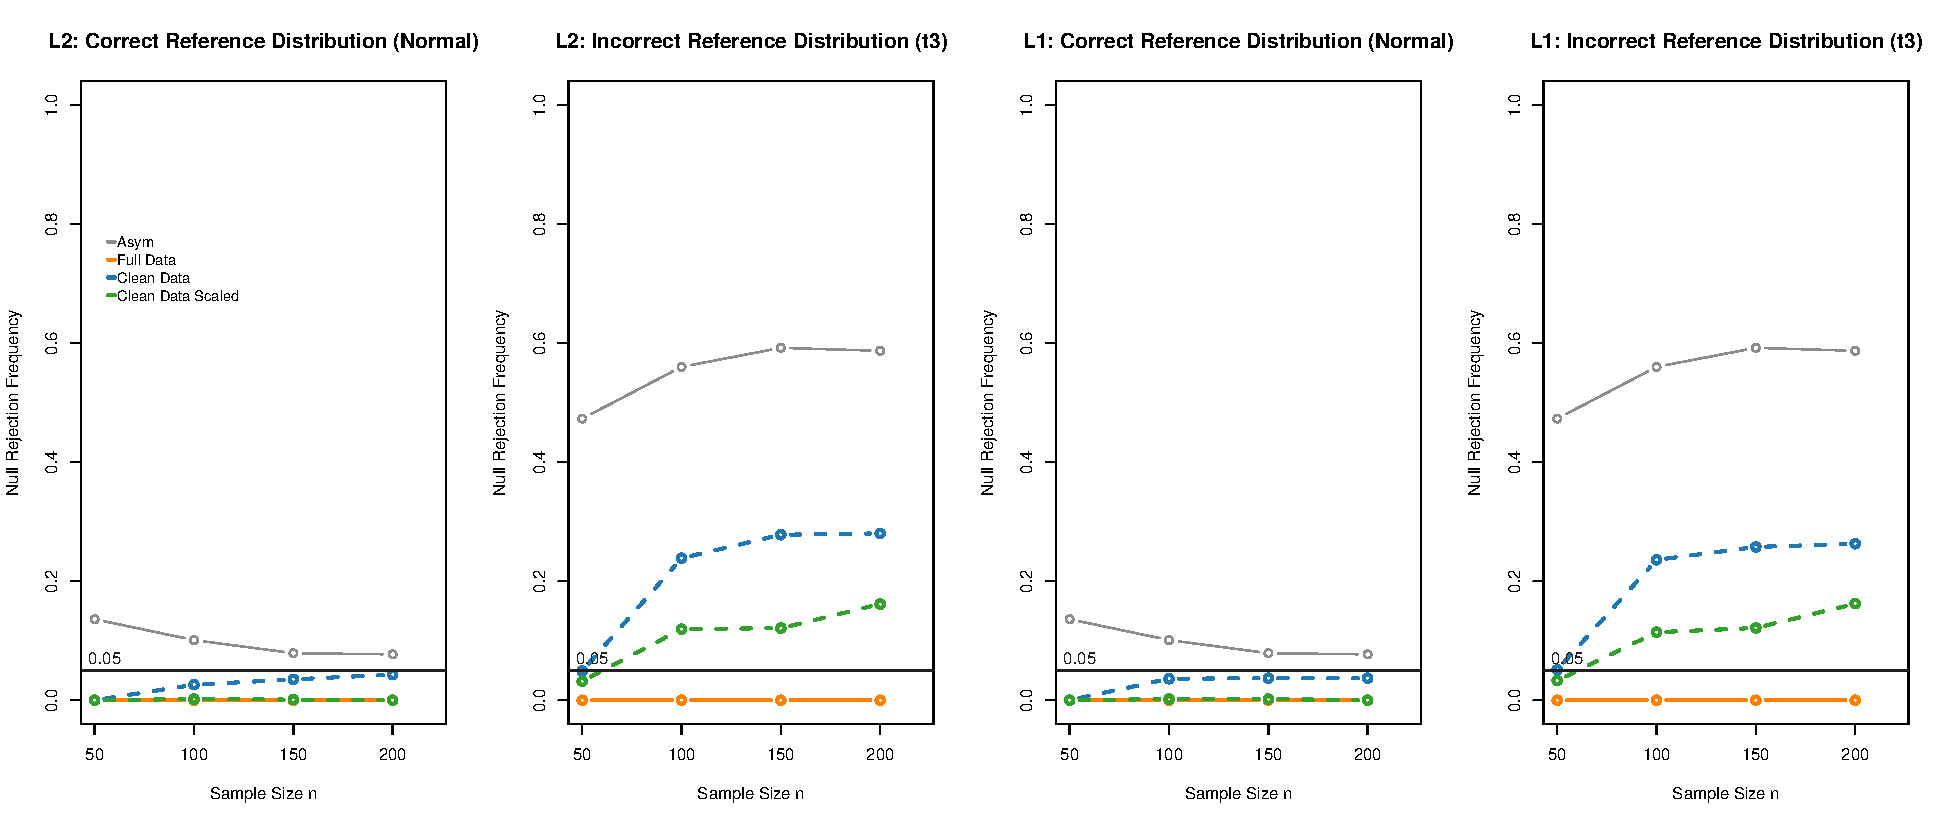
\includegraphics[scale=0.5]{boot_null.pdf}
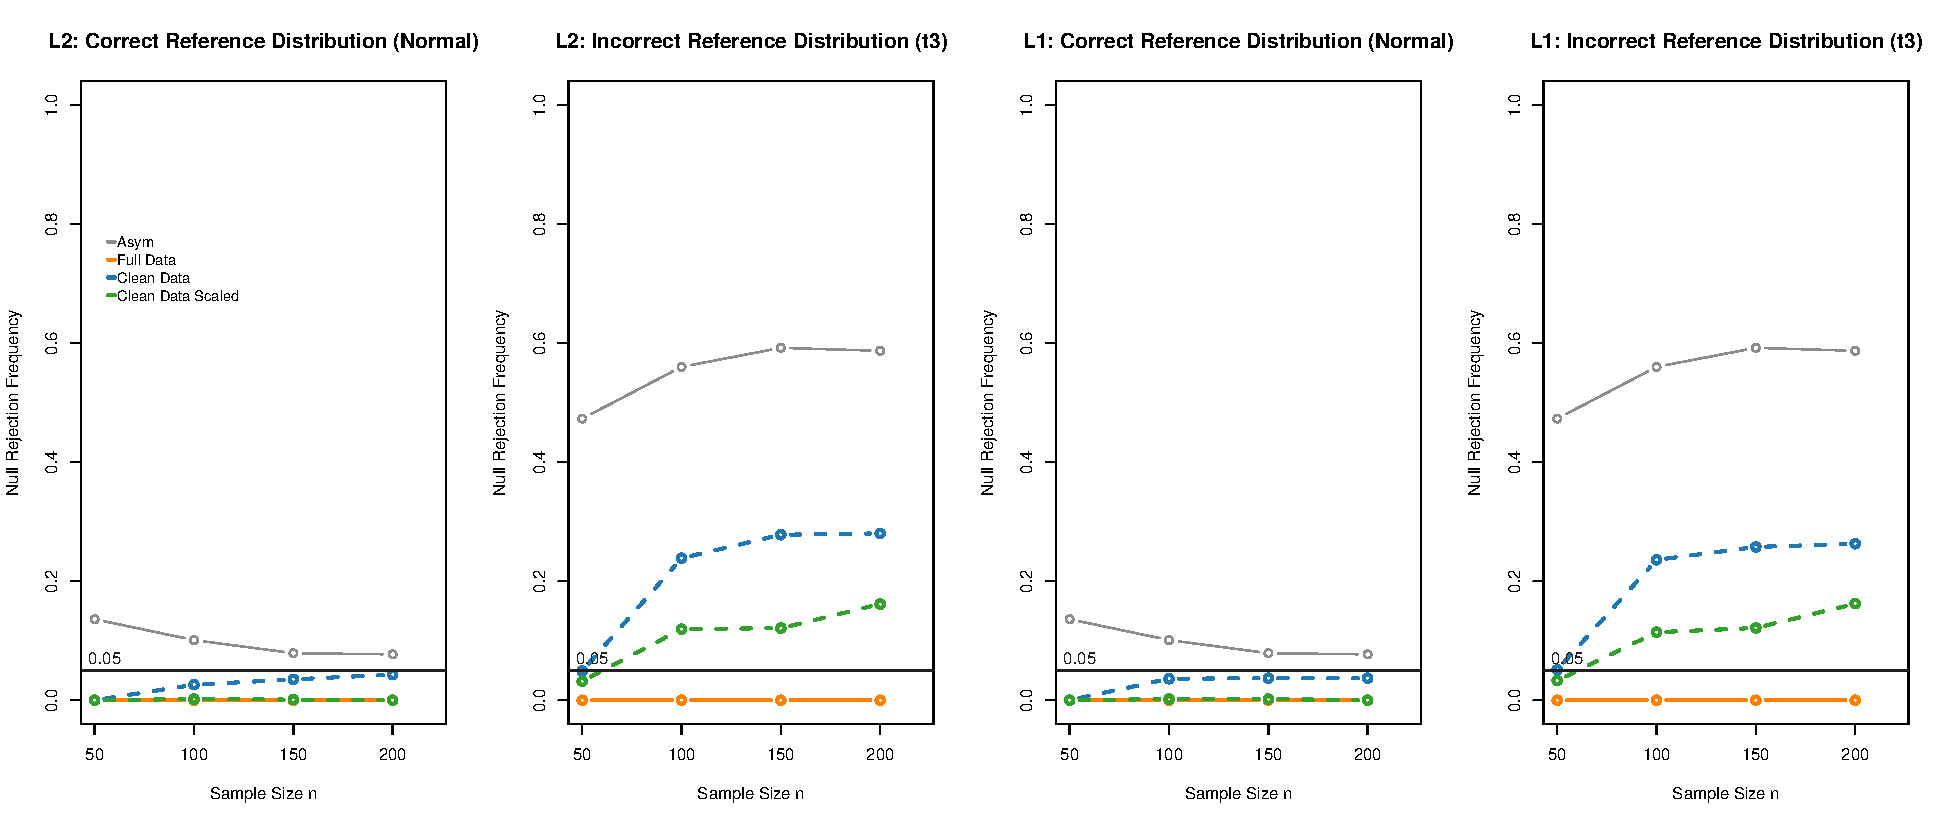
\includegraphics[width=\textwidth]{boot_null.pdf}
\caption{Simulation performance of the bootstrap tests under the null of no distortion when the reference distribution does and does not match the error distribution in the DGP.}
\label{fig_boot_sim_null}
\end{figure}

\subsection{Simulation Performance in the Presence of Distortion}
We assess the performance of the test in the presence of outlier distortion by introducing outliers of varying magnitudes to the DGP, varying the sample size and  degree of autocorrelation in the dependent variable. We plot the null-rejection frequencies for different simulation specifications in Figures \ref{fig_out_sim_alt1} and \ref{fig_out_sim_alt2} for iid and stochastically trending dependent variables when the sample contains 10\% of contaminated observations. To capture the degree of distortion we plot the null rejection frequency against the euclidian distance of all estimated (OLS) coefficients from their true underlying DGP counterparts, scaled by the maximum distance. As the results show, regardless of whether $y$ is iid or stochastically-trending, the power of the test increases with the degree of outlier distortion.  Consistent with our expectations, power also increases with sample size. Additional simulation results with varying proportions of outlier contamination and varying degrees of persistence in $y$ are provided in the appendix.

\begin{figure}[!htbp]  %\vspace{-.35in}
\centering
%\includegraphics[scale=0.6]{{alt_ar0_nreg5_palpha0.05_distnorm_outprop0.1}.pdf}
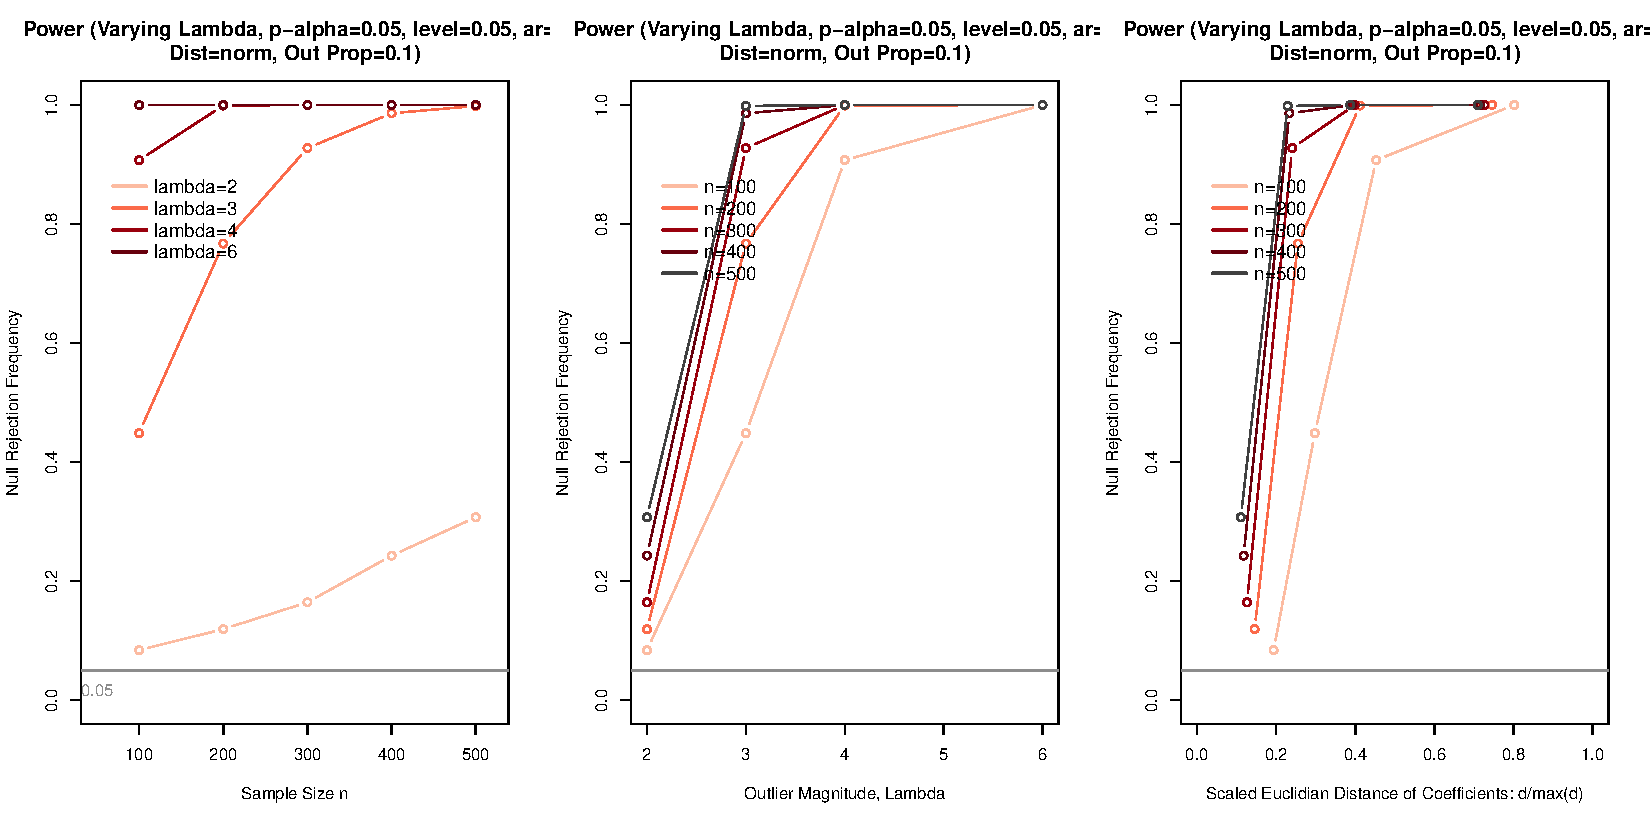
\includegraphics[width = \textwidth]{alt_ar0_nreg5_palpha0.05_distnorm_outprop0.1.pdf}
\caption{Simulation performance under the alternative for varying sample sizes and outlier magnitudes when the dependent variable exhibits no autocorrelation and 10\% of the sample is outlier-contaminated.}
\label{fig_out_sim_alt1}
\end{figure}

\begin{figure}[!htbp]  %\vspace{-.35in}
\centering
%\includegraphics[scale=0.6]{{alt_ar1_nreg5_palpha0.05_distnorm_outprop0.1}.pdf}
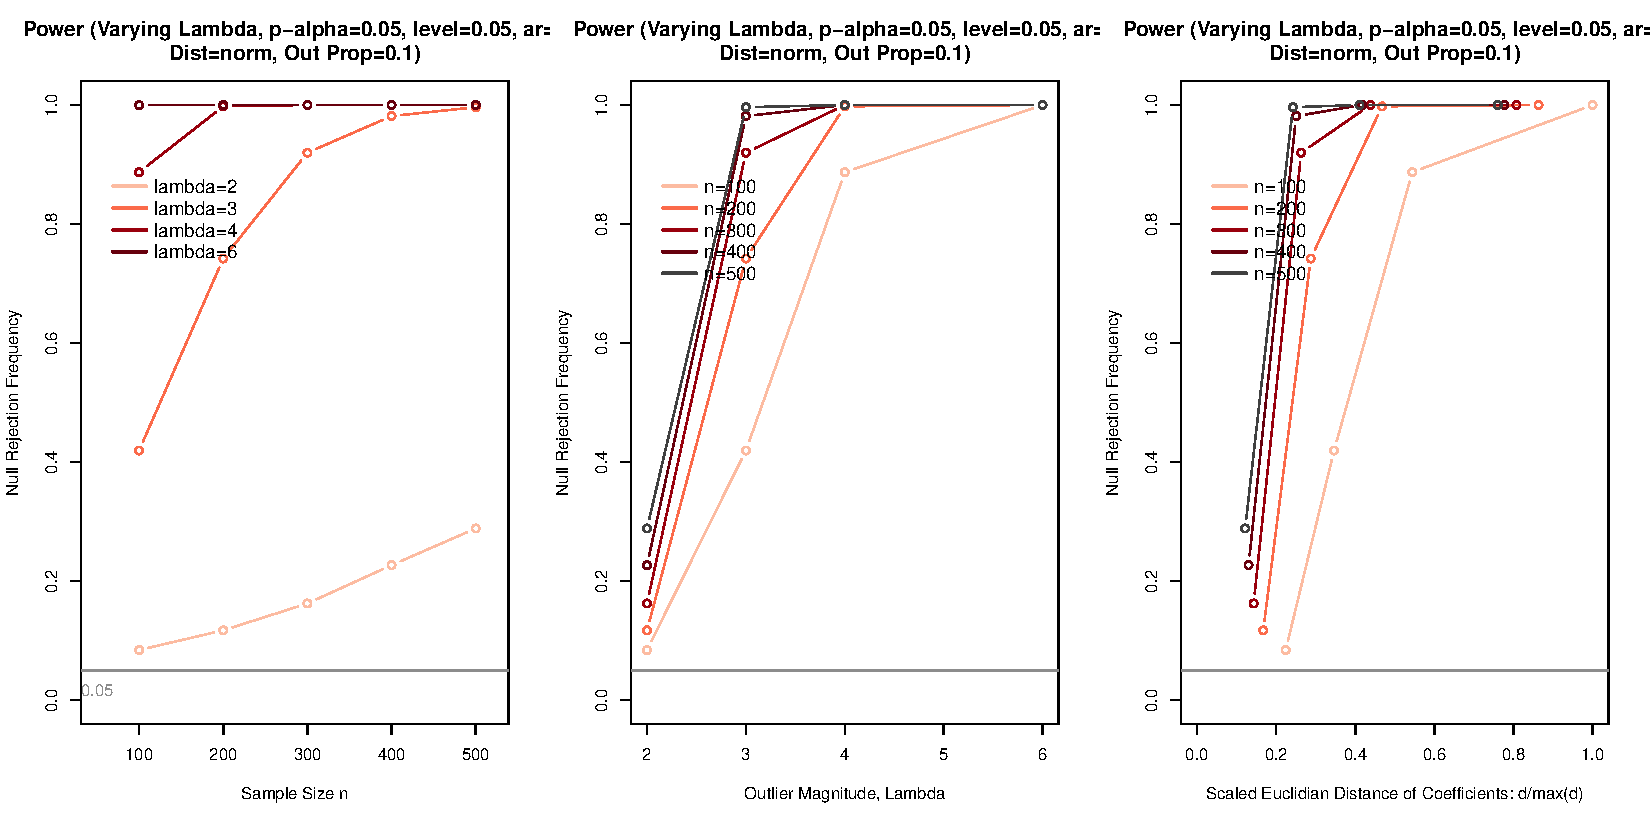
\includegraphics[width = \textwidth]{alt_ar1_nreg5_palpha0.05_distnorm_outprop0.1.pdf}
\caption{Simulation performance under the alternative for varying sample sizes and outlier magnitudes when the dependent variable is stochastically trending and 10\% of the sample is outlier-contaminated.}
\label{fig_out_sim_alt2}
\end{figure}

Bootstrap results are shown in Figures \ref{fig_out_sim_alt_boot4} and \ref{fig_out_sim_alt_boot6} for different outlier magnitudes. As expected, bootstrapping using the raw data appears to have zero power as each bootstrap draw has a chance of including some outlying observations, thus rendering the resulting bootstrap distribution of the L1 or L2 norms uninformative when compared to the original test statistic. In turn, bootstrapping the clean (outlier-removed) data, or the clean data with re-scaled threshold shows desirable power properties: power increases with the sample size as well as with the degree of outlier distortion, even when the reference distribution is non-normal.

\begin{figure}[!htbp]  %\vspace{-.35in}
\centering
%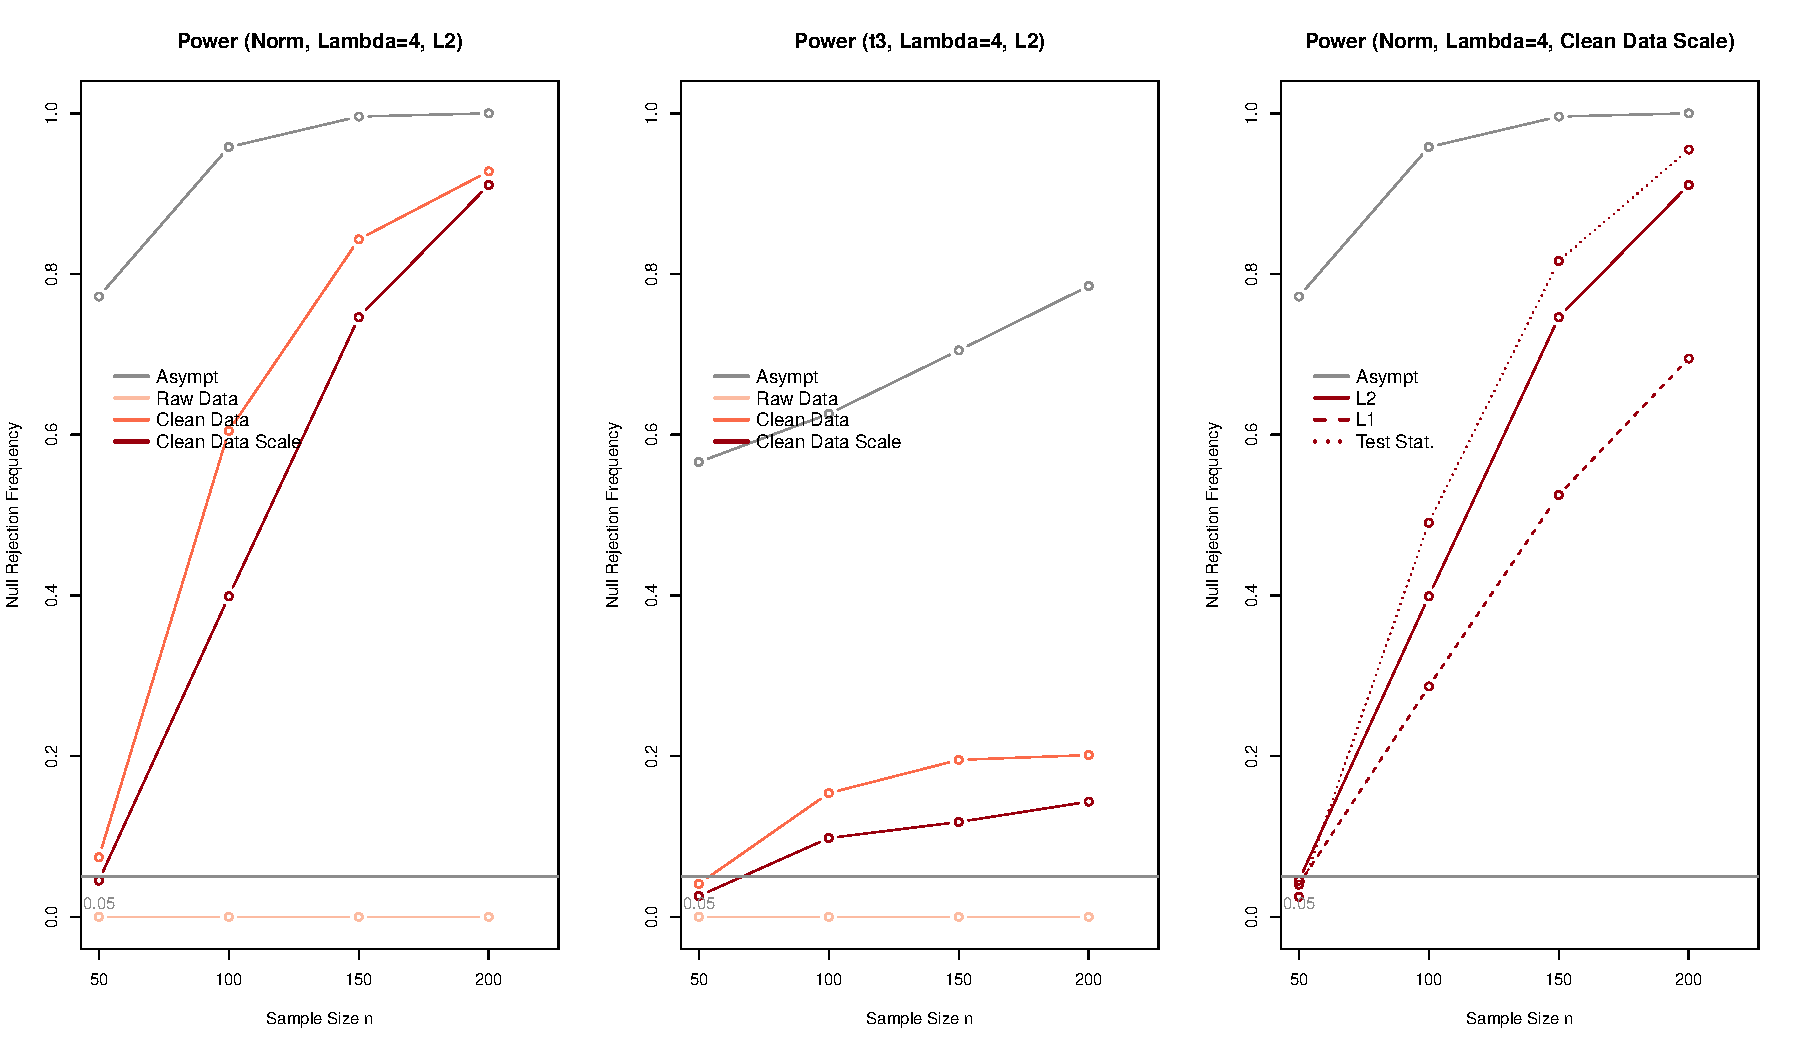
\includegraphics[scale=0.5]{boot_alt_lambda4.pdf}
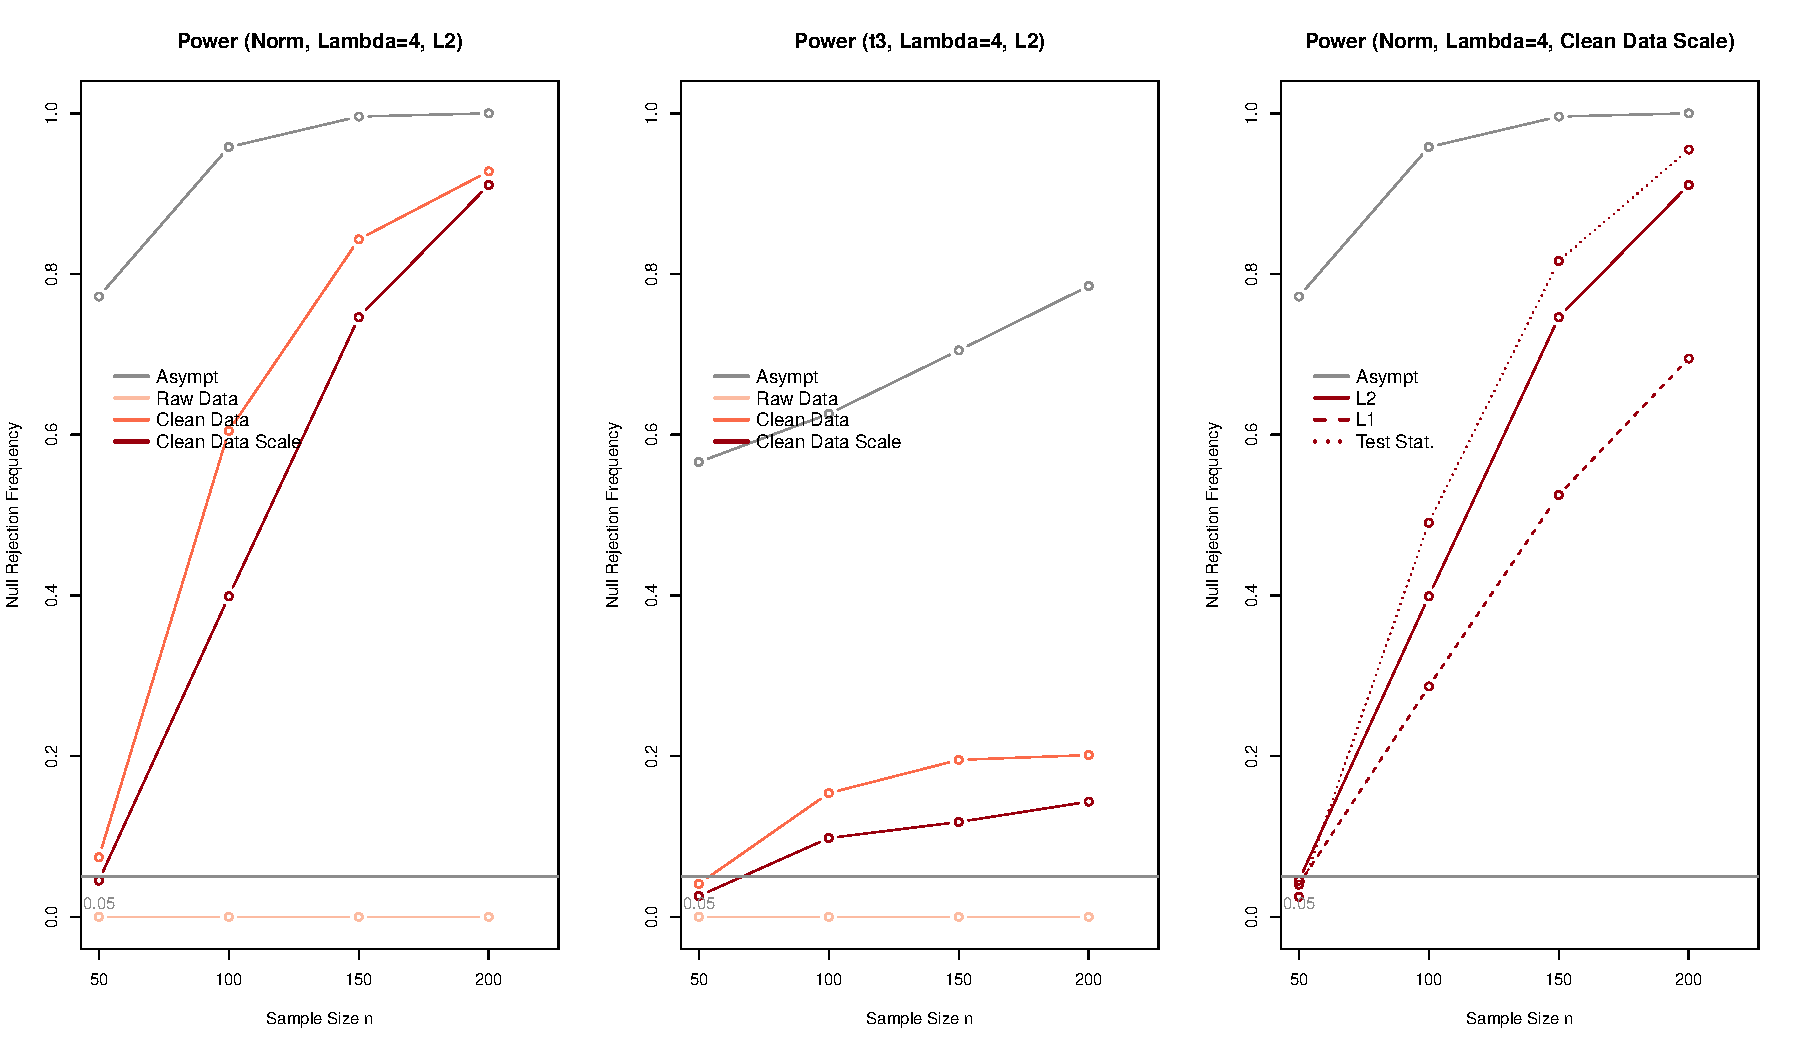
\includegraphics[width = \textwidth]{boot_alt_lambda4.pdf}
\caption{Simulation performance under the alternative for varying sample sizes when using the bootstrap implementations of our test (for outlier magnitude of 4SD of the error term).}
\label{fig_out_sim_alt_boot4}
\end{figure}

\begin{figure}[!htbp]  %\vspace{-.35in}
\centering
%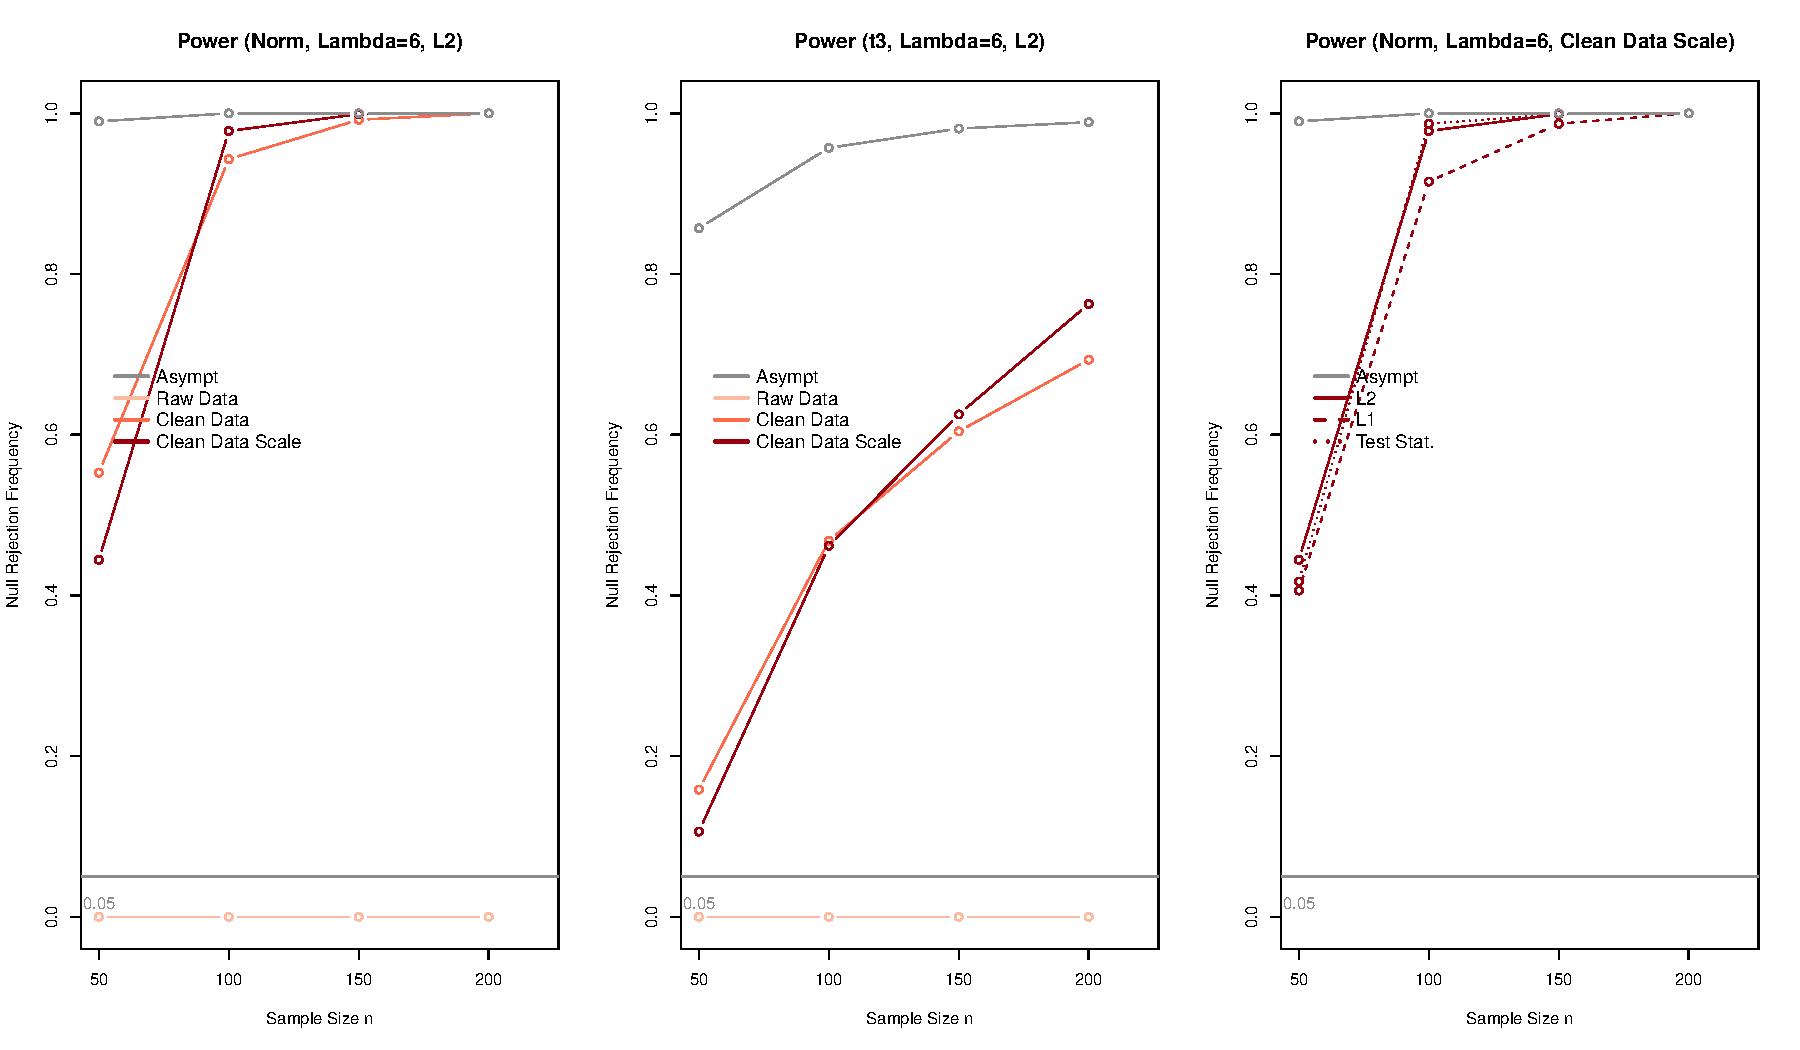
\includegraphics[scale=0.5]{boot_alt_lambda6.pdf}
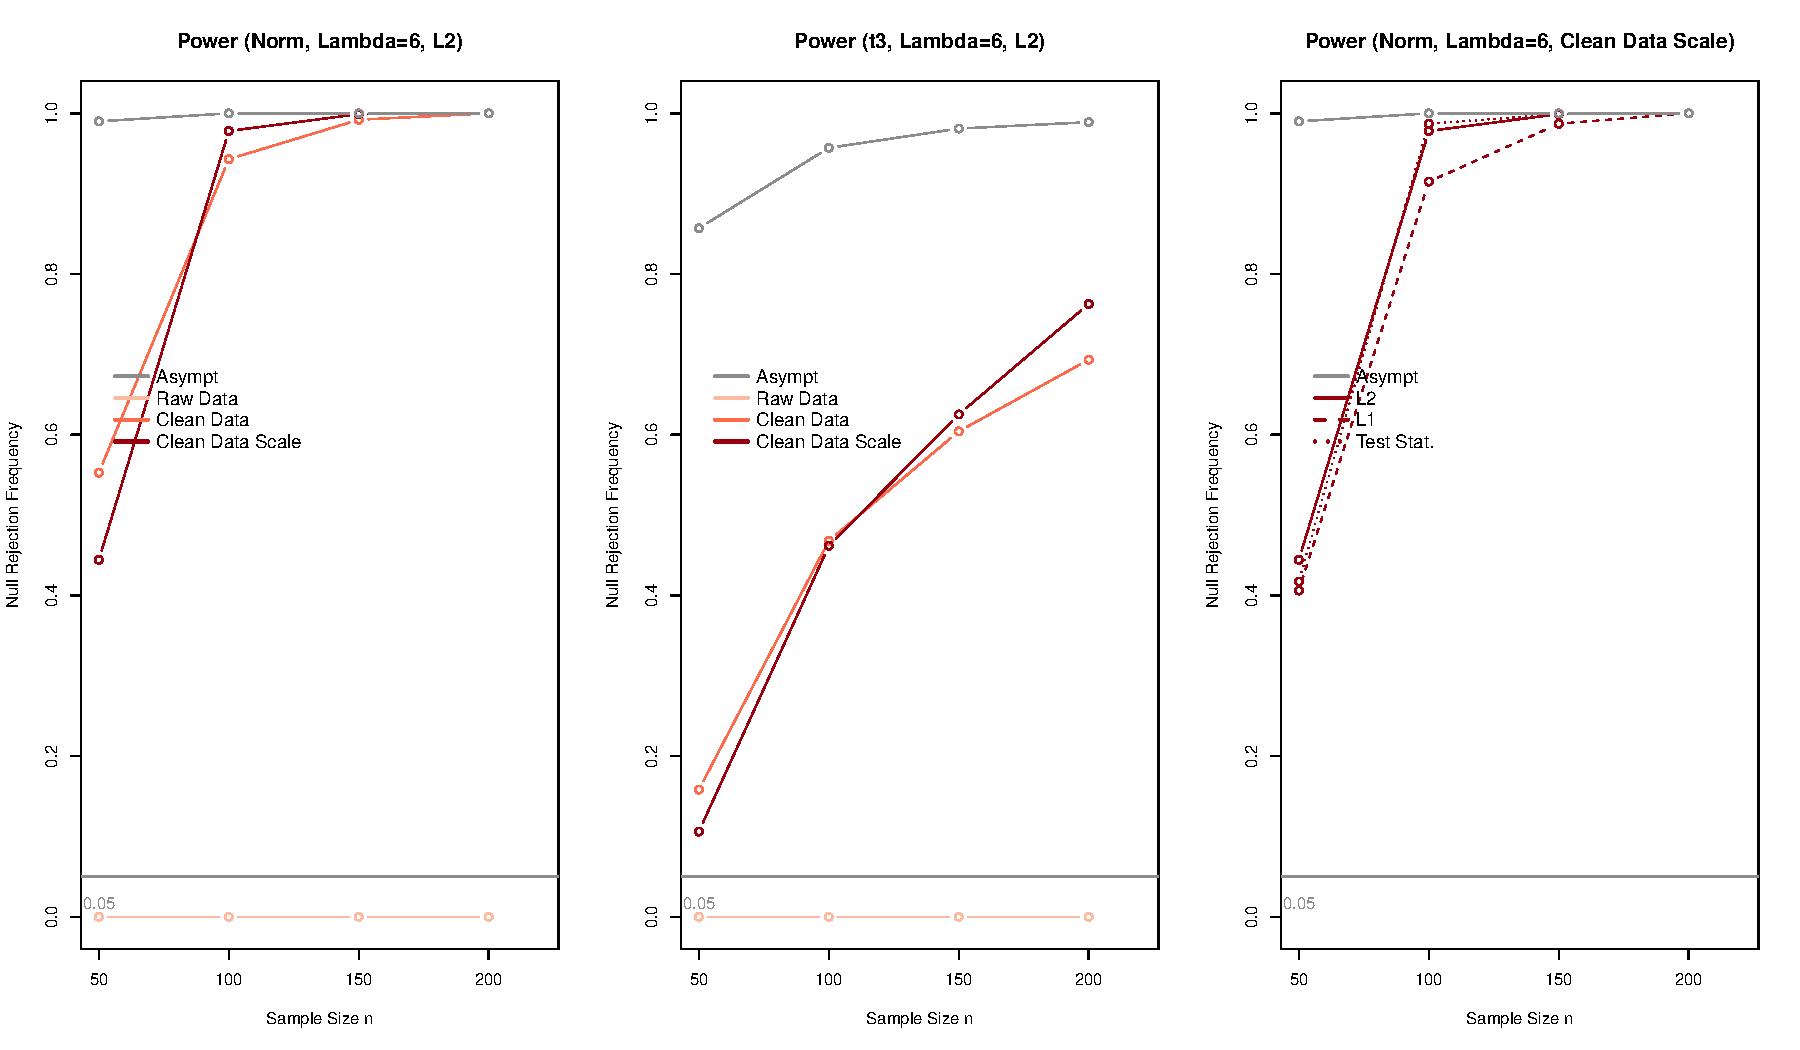
\includegraphics[width = \textwidth]{boot_alt_lambda6.pdf}
\caption{Simulation performance under the alternative for varying sample sizes when using the bootstrap implementations of our test (for outlier magnitude of 6SD of the error term).}
\label{fig_out_sim_alt_boot6}
\end{figure}

\subsection{Summary of Simulation Results}
The simulation results show well-controlled size and high power of our asymptotic test in large samples (n $>$ 200), with the tests being slightly oversized in small samples (n $<$ 200). In line with our theory results, the performance of the test is unaffected by the presence of stochastic trends. Bootstrapping the cleaned (outlier-removed) data, or bootstrapping with scaled significance levels on the cleaned data performs well under the null of no outliers, and reduces size-distortions of the asymptotic test in small samples and when the reference distribution is different to the assumed distribution. These bootstrap approaches also exhibit good power under a range of alternatives. We do not recommend bootstrapping the raw data, as expected, re-sampling the raw data has close to no power to detect distortion.


%\clearpage

\section{Application: Climate Adaptation \& \\ the Macro-Economic Impacts of Temperatures} \label{sec_application}
We apply the outlier distortion test to estimates of the economic impacts of climate change allowing for income-driven adaptation. Specifically, we use the robust IIS estimator to estimate a panel model of the effects of temperature on GDP per capita growth using a global panel dataset in line with the existing climate-econometric impacts literature \cite[e.g.][]{burke2015global, dell2012temperature, pretis2018uncertain}. While existing estimates strongly support a non-linear relationship between GDP per capita growth and temperatures, adaptation to climate change has been notably absent in empirical macro-economic cross-country analyses. Higher incomes might mitigate the impacts of climate change \citep[see e.g. ][]{acevedo2020effects, schwarz2020modelling}, and such adaptation might bias existing historical estimates and subsequent future projections of macro-economic climate impacts. We therefore estimate a panel model of climate impacts while allowing for adaptation driven by incomes, specified through interaction terms of temperatures and (lagged) log GDP per capita.

A concern with global panel-econometric models of climate impacts is the inability to account for all observed variation in economic growth. Even though conventional panel climate impact models control for time fixed effects, country fixed effects, and country-specific (non-linear) time trends, there are potentially numerous un-modelled idiosyncratic shocks. Such shocks -- taking the form of outliers in the model -- can erroneously be attributed to climate variation and thus distort the estimated coefficients on climate variables. To account for the presence of such un-modelled shocks, we estimate our panel climate impacts model with adaptation using both OLS and the robust IIS estimator and subsequently test whether there is evidence of coefficient distortion using our proposed outlier distortion test.

\subsection{Data \& Model}
Following the macro-econometric literature studying the temperature effects on economic growth, we model the change in the log of real GDP per capita \cite[World Development Indicators, ][]{rld2019world} from 1961-2017 for 169 countries as a function of population-weighted climate variation. We obtain historical climate observations on temperatures and precipitation from \citep[][ version 5]{matsuura2018terrestrial} covering global land areas at a 0.5$^\circ$ spatial resolution. To map gridded climate observations to individual countries in each year, we weight climate observations by gridded population data \citep{ciesin2016gridded} at the same spatial resolution. Population-weighting (rather than area-weighting) is more likely to capture the effects of climate onto socio-economic activity \citep[see ][]{tol2017population}. To project climate impacts to the end of the century, we construct a dataset of country-level changes in temperature based on CMIP5 climate models \citep{taylor2012overview} and use long-term country-level forecasts of GDP per capita for our baseline \citep{muller2019econometric}. In the appendix, we also consider the impact of precipitation (see Figure (\ref{fig_projection_map_withprcp})).

Modelling GDP per capita growth in fixed effects panels as a non-linear (quadratic) function of annual-average temperatures has become common practise in the climate econometric literature. We expand on these existing models by allowing for climate adaptation at different income levels. Specifically, our model allows for adaptation by potentially attenuating (or amplifying) the coefficients on temperatures through interaction terms with (lagged) log of GDP per capita. \citet{dell2012temperature} estimate a simplified version of such a specification by interacting a linear temperature variable with a dummy variable for poor countries, and \citet{burke2015global} explore the interaction of a linear temperature variable with country-level incomes. Here we generalise this to non-linear temperature impacts interacted with the continuum of per capita incomes. A similar approach of estimating income-based adaptation has also been applied for heat-related mortality in \citet{carleton2020valuing} and \citet{schwarz2020modelling} for climate impacts of extremes. Our base model is given in equation (\ref{pan_base}) and our adaptation model is given in equation (\ref{pan_adapt}):

\begin{small}
\begin{equation}
\label{pan_base}
\Delta log(y)_{i,t} = \alpha_i + \lambda_t + \beta_1 T_{i,t} + \beta_2 T^2_{i,t} + x_{i,t}'\gamma + u_{i,t}
\end{equation}
\end{small}


\begin{small}
\begin{equation}
\label{pan_adapt}
\Delta log(y)_{i,t} = \alpha_i + \lambda_t + \beta_1 T_{i,t} + \beta_2 T^2_{i,t} + \beta_3 \left[ T_{i,t} \times  log(y)_{i, t} \right] + \beta_4 \left[  T^2_{i,t} \times  log(y)_{i, t} \right] + x_{i,t}'\gamma + u_{i,t}
\end{equation}
\end{small}

where $\Delta log(y)_{i,t}$ is the year-on-year change in per capita income in country $i$ in year $t$. The coefficients of interest are $\beta_1$ through $\beta_4$. specifically $\beta_1$ and $\beta_2$ capture the (potentially non-linear) impacts on GDP per capita growth and coefficients $\beta_3$, $\beta_4$ on interactions terms allow for the temperature-growth relationship to vary by country incomes. The vector $x_{i,t}$ denotes a set of control variables including population-weighted annual average precipitation (and its square), and country-specific linear and quadratic trends as in \citet{burke2015global} and \citet{pretis2018uncertain}.

To assess the impact of unknown idiosyncratic shocks, we estimate equations (\ref{pan_base}) and (\ref{pan_adapt}) using OLS (as is convention in the literature) and then compare the OLS estimates to those obtained when estimating equations (\ref{pan_base}) and (\ref{pan_adapt}) using the robust IIS estimator. Let $\tilde{\beta}$ denote the vector of coefficients estimated by OLS $\tilde{\beta}=(\tilde{\beta}_1, \tilde{\beta}_2, \tilde{\beta}_3, \tilde{\beta}_4)$, and $\hat{\beta}^{( 1)}_{c}$ denote the vector of coefficients estimated using the robust IIS estimator at $\gamma_{c=2.57}=0.01$ relative to a normal reference distribution ${\sf f}$. The hypothesis of interest is $H_0: \tilde{\beta} = \hat{\beta}^{( 1)}_{c}$. In other words, we assess possible outlier distortion in the coefficient estimates. To alleviate concerns of endogeneity between $\Delta log(y)_{i,t}$ and $log(y)_{i, t}$, we also present a model using $log(y)_{i, t-1}$ in the Appendix (see equation (\ref{pan_adapt.L1})).
For all IIS estimates, we apply a variance correction, which is contained in the \texttt{isatvar} function of the \texttt{gets} package.\ignore{@Felix can you provide more information here please?}

\subsection{Results}

The estimation results (see Figure \ref{tab_app1_estimates}) show conventional OLS panel estimates of this relationship are significantly different to those obtained using the robust estimator. We identify 165 and 170 outliers for the base (see equation (\ref{pan_base})) and the adaptation model (see equation (\ref{pan_adapt})). We present the distribution of the detected outlying observations in the panel model over time, countries, and both (Figures \ref{fig_out_app1} and \ref{fig_map_app1}). The number of detected outliers greatly exceeds the number expected by chance. In total, 165 and 170 country-year observations were identified as outlying compared to 77.16 expected under the null when there are no outliers. The observed proportion of outliers $\hat{\gamma}_{c=2.57}= 165/7716=0.021$ and $\hat{\gamma}_{c=2.57}= 170/7716=0.022$ is statistically different from the expected proportion of $\gamma_{c=2.57}=0.01$ ($p<0.001$ using the \citet{jiao2018testing} proportion test comparing 0.021 and 0.022 to 0.01).

Further, the distribution of outliers does not appear to be random over time and space -- no outliers are detected for OECD countries as all outliers are detected in developing countries and economies in transition (see Figure \ref{fig_map_app1}). While further investigation of outlier cause and type is beyond the scope of this paper, we note that there is a temporal cluster coinciding with the collapse of the Soviet Union and the onset of the first Gulf War \ref{fig_out_app1}), which may well capture an idiosyncratic shock not modelled in the base panel model.
%Beyond distortion in coefficients,
Figure \ref{fig_dist_coef_app1} shows the difference in estimated coefficients between the robust IIS approach and OLS. Specifically, the robust coefficient estimates are attenuated relative to the OLS estimates. The difference between the OLS and robust IIS estimates is statistically different from zero when applying our proposed test for outlier distortion. Formally, we construct our test statistic for outlier distortion in the four coefficients of interest as:
\begin{eqnarray}
H^{1}_{(n,c)} = n \left( \hat{\beta}^{( 1)}_{c} - \tilde{\beta} \right)'\widehat{\mbox{avar}}\left( \hat{\beta}^{( 1)}_{c} - \tilde{\beta} \right)^{-1}\left( \hat{\beta}^{( 1)}_{c} - \tilde{\beta} \right)
\end{eqnarray}
where $c=1.96$ for a normal reference distribution and a sample size of $n=7716$. The outlier test statistic for each coefficient and all temperature coefficients of interest are shown in Table \ref{tab_app1_estimates} (third and sixth column). We compare the resulting test statistic $H^{1}_{(n,c)} = 111.27$ for our base model against the critical values of the $\chi^{2}$ distribution with $df=2$ and for our adaptation model with $H^{1}_{(n,c)} = 770.69$ against the critical values of the $\chi^{2}$ distribution with $df=4$, as we are testing for the distortion of four coefficients. The null hypothesis of no distortion is rejected at any conventional significance level for both models, with $p<0.0001$.

\begin{table}
\caption{OLS and IIS Panel Regression Results together with their difference in coefficients and the resulting outlier distortion test statistic. Coefficients on control variables are omitted.}
\label{tab_app1_estimates}
\centering
\resizebox{\textwidth}{!}{\begin{tabular}[t]{|L{5cm}cc|>{}C{2.5cm}|cc|>{}C{2.5cm}|}
\toprule
  & Base & Base IIS & Base Outlier Distortion Test & Adaptation & Adaptation IIS & Adaptation Outlier Distortion Test\\
\midrule
Temperature & 0.01734*** & 0.01032*** & 108.95 & -0.06224*** & -0.03384*** & 186.25\\
 & (0.00348) & (0.00233) & [$<$0.001] & (0.01041) & (0.0072) & [$<$0.001]\\
Temperature\textsuperscript{2} & -0.00059*** & -0.00039*** & 99.05 & 0.00070 & 0.00001 & 88.57\\
 & (0.0001) & (0.00007) & [$<$0.001] & (0.00037) & (0.00026) & [$<$0.001]\\
Precipitation & 0.00043 & 0.00073 & 1.98 & 0.01018 & 0.01328*** & 7.86\\
 & (0.00111) & (0.00074) & [0.160] & (0.00563) & (0.00383) & [0.005]\\
Precipitation\textsuperscript{2} & -0.00004 & -0.00004 & 0.46 & -0.00019 & -0.00035** & 17.55\\
 & (0.00003) & (0.00002) & [0.496] & (0.00019) & (0.00013) & [$<$0.001]\\
Temperature x GDP\textsubscript{pc} &  &  &  & 0.00811*** & 0.00416*** & 317.59\\
 &  &  &  & (0.00111) & (0.00077) & [$<$0.001]\\
Temperature\textsuperscript{2} x GDP\textsubscript{pc} &  &  &  & -0.00012** & -0.00002 & 148.17\\
 &  &  &  & (0.00004) & (0.00003) & [$<$0.001]\\
Precipitation x GDP\textsubscript{pc} &  &  &  & -0.00121 & -0.00155*** & 6.86\\
 &  &  &  & (0.00066) & (0.00045) & [0.009]\\
Precipitation\textsuperscript{2} x GDP\textsubscript{pc} &  &  &  & 0.00002 & 0.00004* & 17.52\\
 &  &  &  & (0.00002) & (0.00002) & [$<$0.001]\\
\midrule
Num. Outliers &  &  & 165 &  &  & 170\\
Outlier Distortion test statistic for Temp. Variables &  &  & $\chi^2_{2}$ = 111.27
[$<$0.001] &  &  & $\chi^2_{4}$ = 770.69
[$<$0.001]\\
Num.Obs. & 7716 & 7716 &  & 7716 & 7716 & \\
BIC & -18483.2 & -23533.1 &  & -18801.4 & -23776.0 & \\
Log.Lik. & 11774.742 & 15038.149 &  & 11951.758 & 15199.897 & \\
Fixed Effects & Country \& Year & Country \& Year &  & Country \& Year & Country \& Year & \\
\bottomrule
\multicolumn{7}{l}{\textsuperscript{} * p $<$ 0.05, ** p $<$ 0.01, *** p $<$ 0.001}\\
\multicolumn{7}{l}{\textsuperscript{} (Standard Errors) and [p-values]}\\
\end{tabular}}
\end{table}

\begin{figure}[!htbp]  %\vspace{-.35in}
\centering
%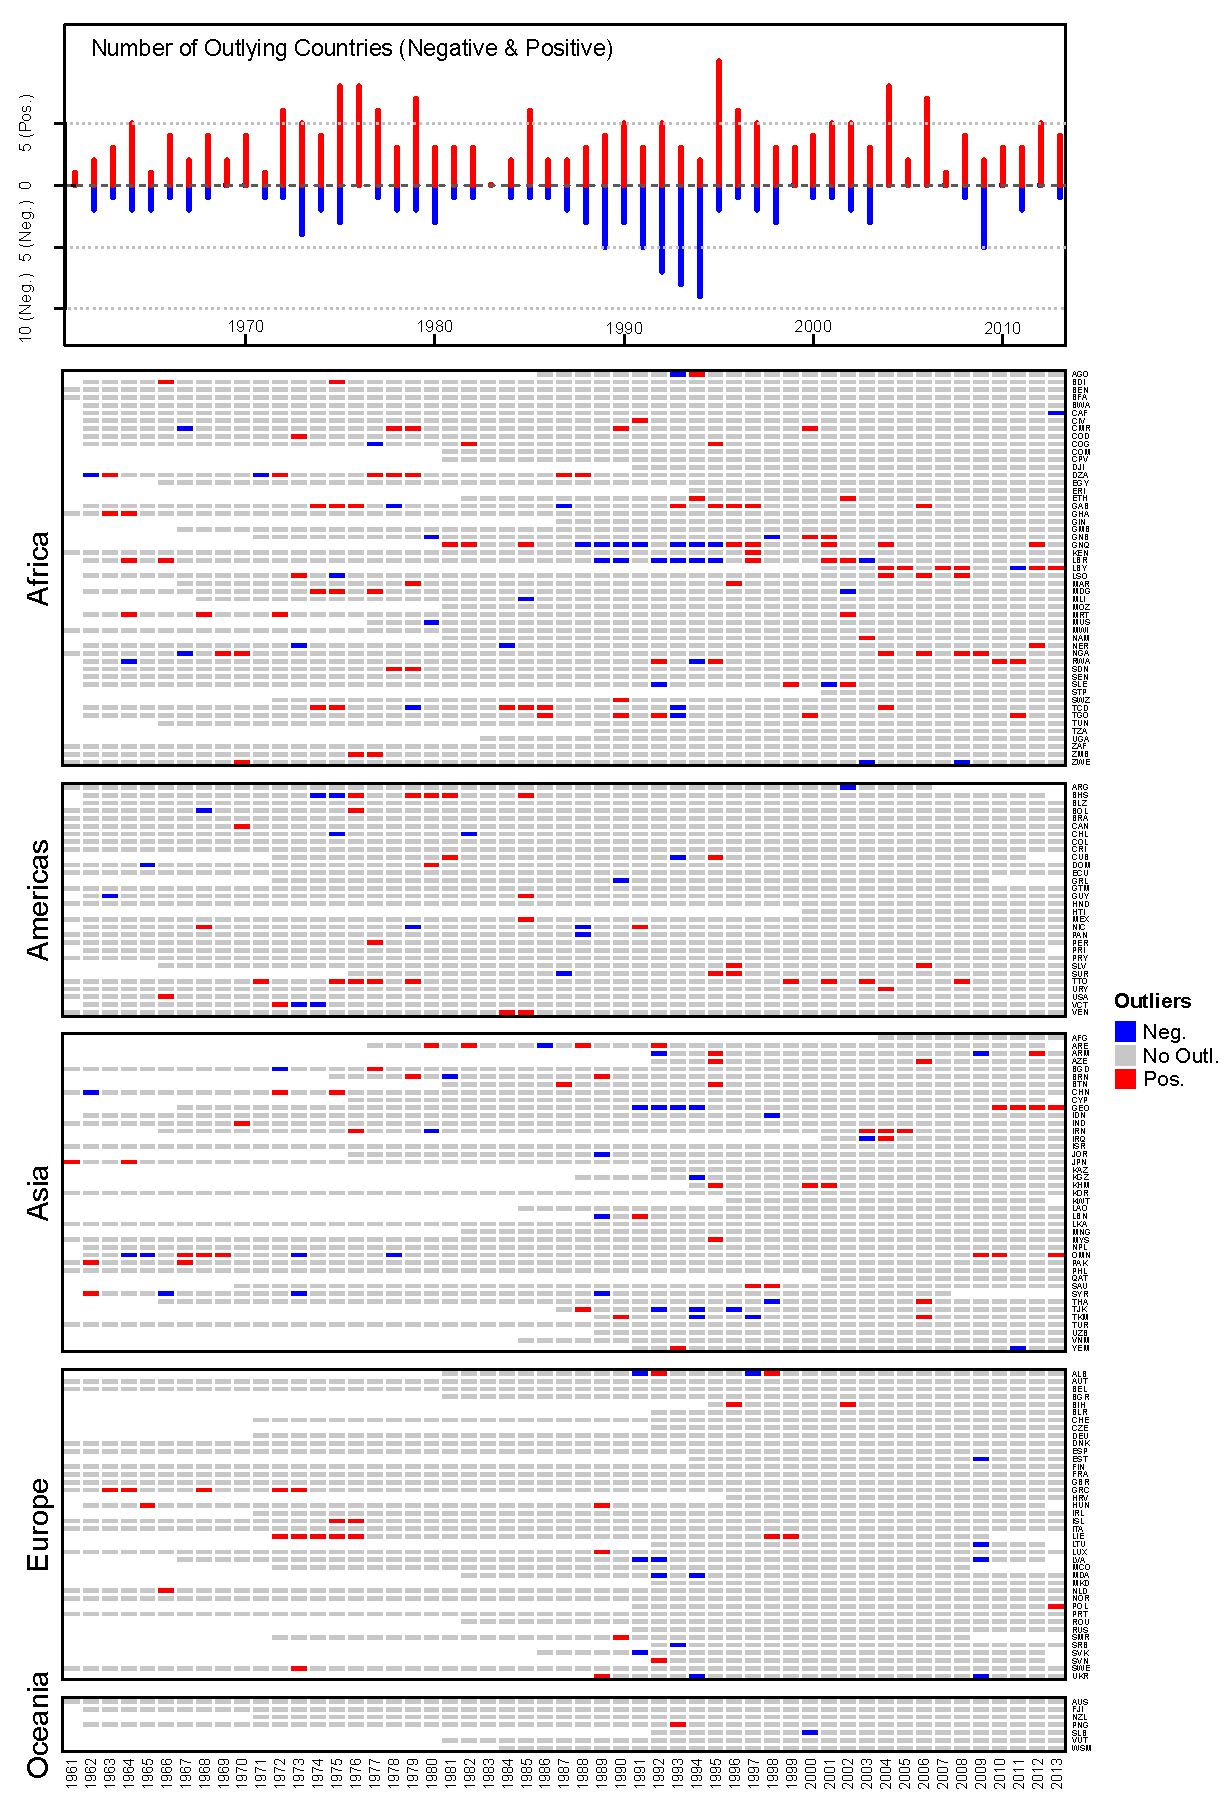
\includegraphics[scale=0.7]{heat1_lag_v1_edited.pdf}
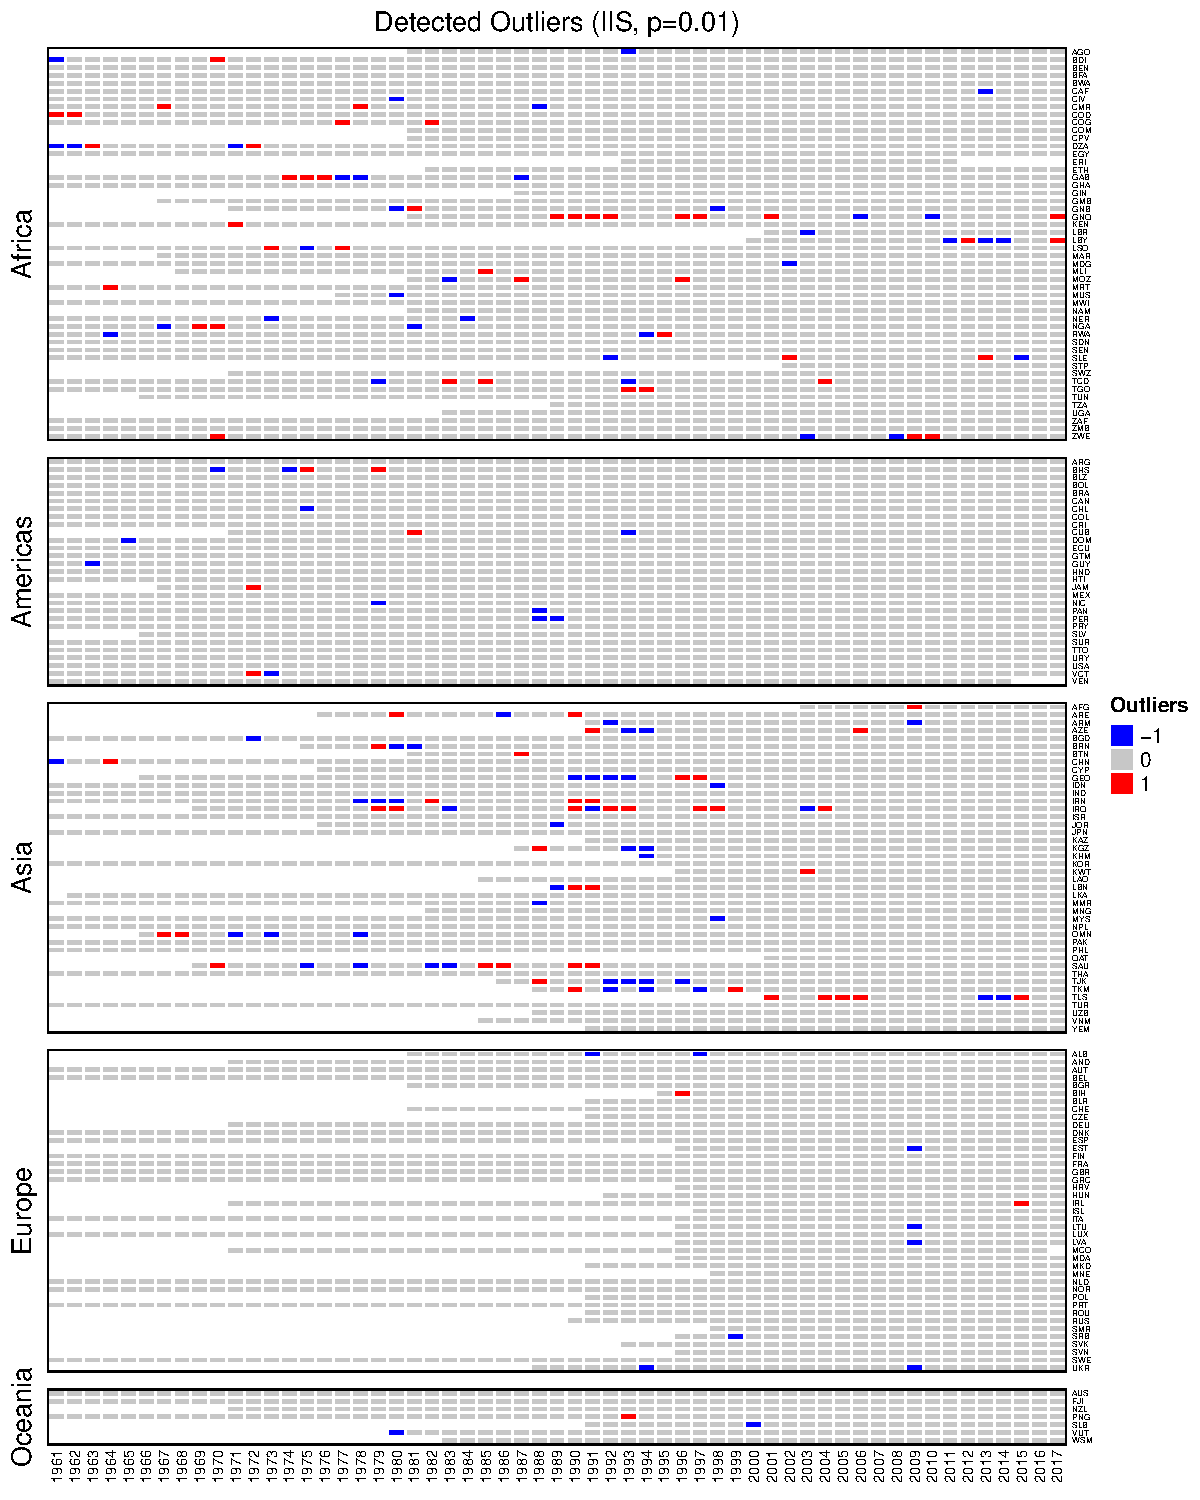
\includegraphics[width = \textwidth]{heat1_adapt.pdf}
\caption{Detected Outliers using the robust IIS estimator across countries and time in the global cross-country panel from 1961-2017 in the adaptation model. Top Figure panel shows the number of positive (red) and negative (blue) outliers aggregated over countries in each year. Bottom panel shows country-year observations as gray when not outlying, blue when there is a negative outliers, and red for positive outliers.}
\label{fig_out_app1}
\end{figure}

\begin{figure}[!htbp]  %\vspace{-.35in}
\centering
%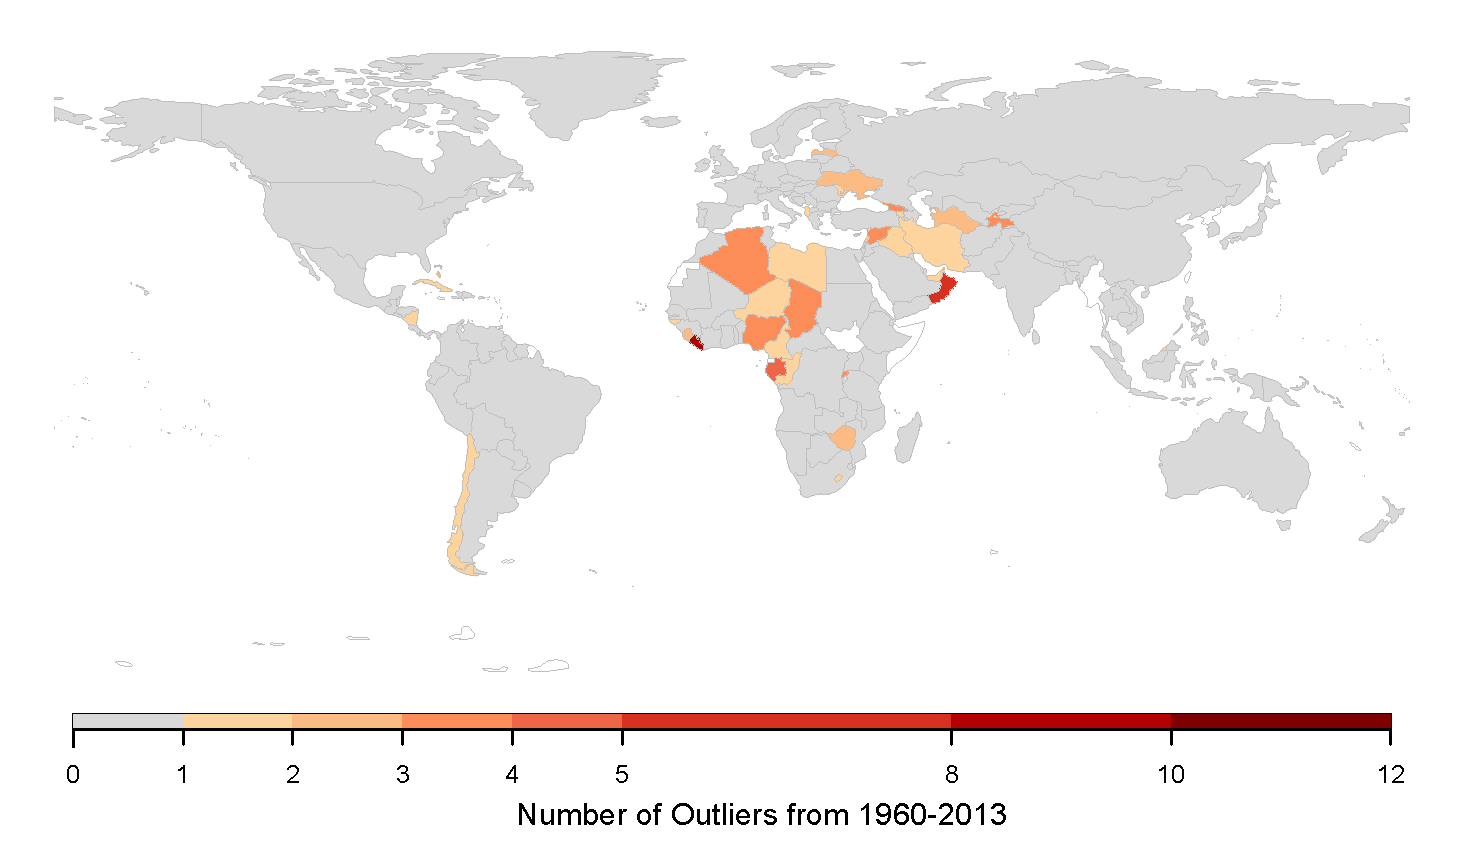
\includegraphics[scale=0.6]{ctry_map_lag_edited.pdf}
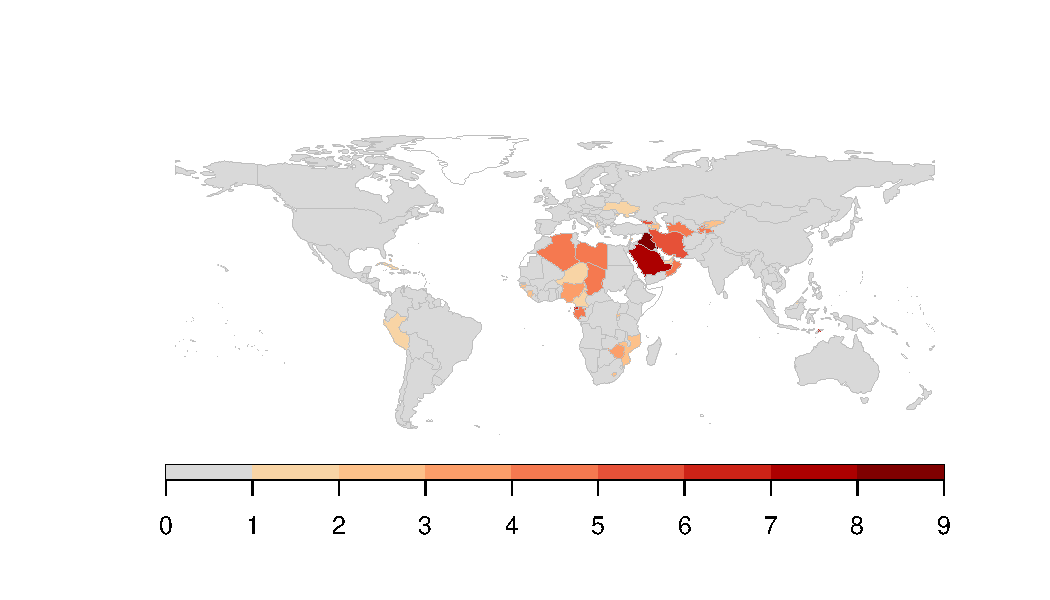
\includegraphics[width = \textwidth]{ctry_map_adapt.pdf}
\caption{Detected outliers aggregated over the full sample of 1961 - 2017 by country in the panel in the adaptation model. Gray denotes no outliers detected.}
\label{fig_map_app1}
\end{figure}

\clearpage

We further show significant evidence of income-driven adaptation to temperatures (Figures \ref{fig_dist_coef_app1} and \ref{fig_dist_app1}), however, the estimates are similarly distorted by the presence of outlying observations as in our base model. Richer countries exhibit a different response function to temperatures compared to poor and middle-income countries, but the shape of the estimated effects overall shows a dampened temperature impact for the robust estimator compared to OLS. This suggests that richer countries will be significantly more able to deal with the consequences of climate change. Such a dynamic could exacerbate existin cross-country inequality with continued climate change.

We show the estimated non-linear relationship between temperatures and growth for three different income levels (25\textsuperscript{th}, 50\textsuperscript{th}, and 75\textsuperscript{th} income percentiles) in Figure \ref{fig_dist_app1}. Results across income levels show that controlling for outlying observations dampens the impacts of temperatures onto economic growth.



\begin{figure}[!htbp]  %    \vspace{-.35in}
\centering
%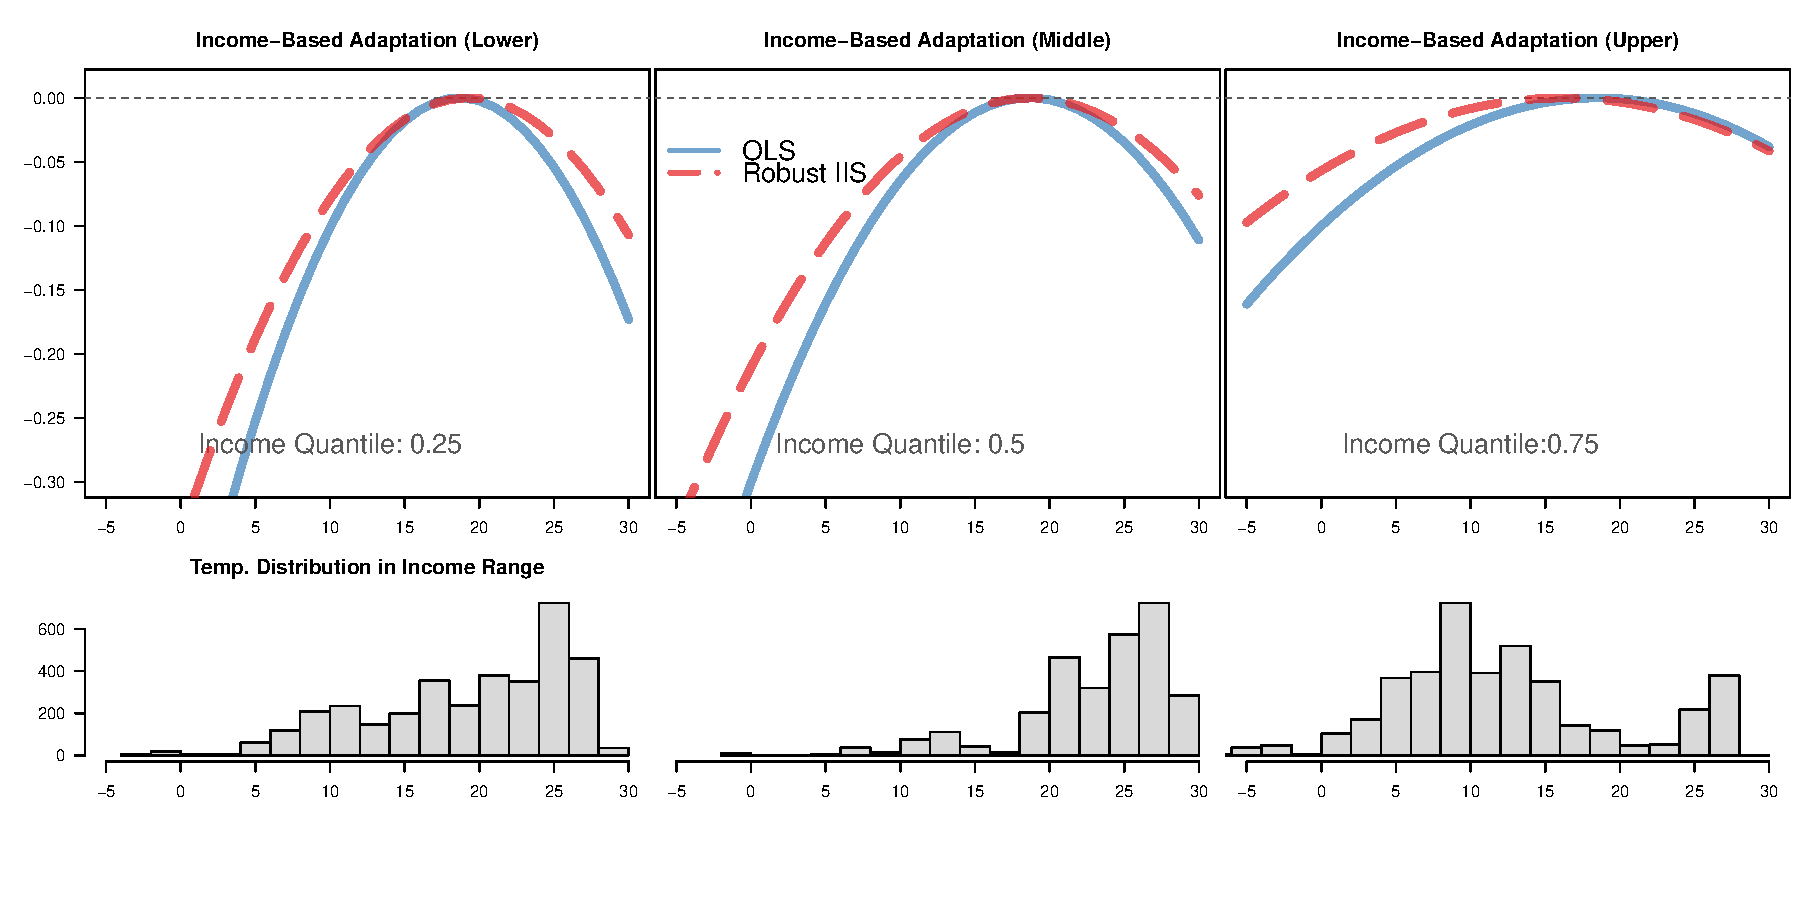
\includegraphics[scale=0.55]{eff_v1_lag.pdf}
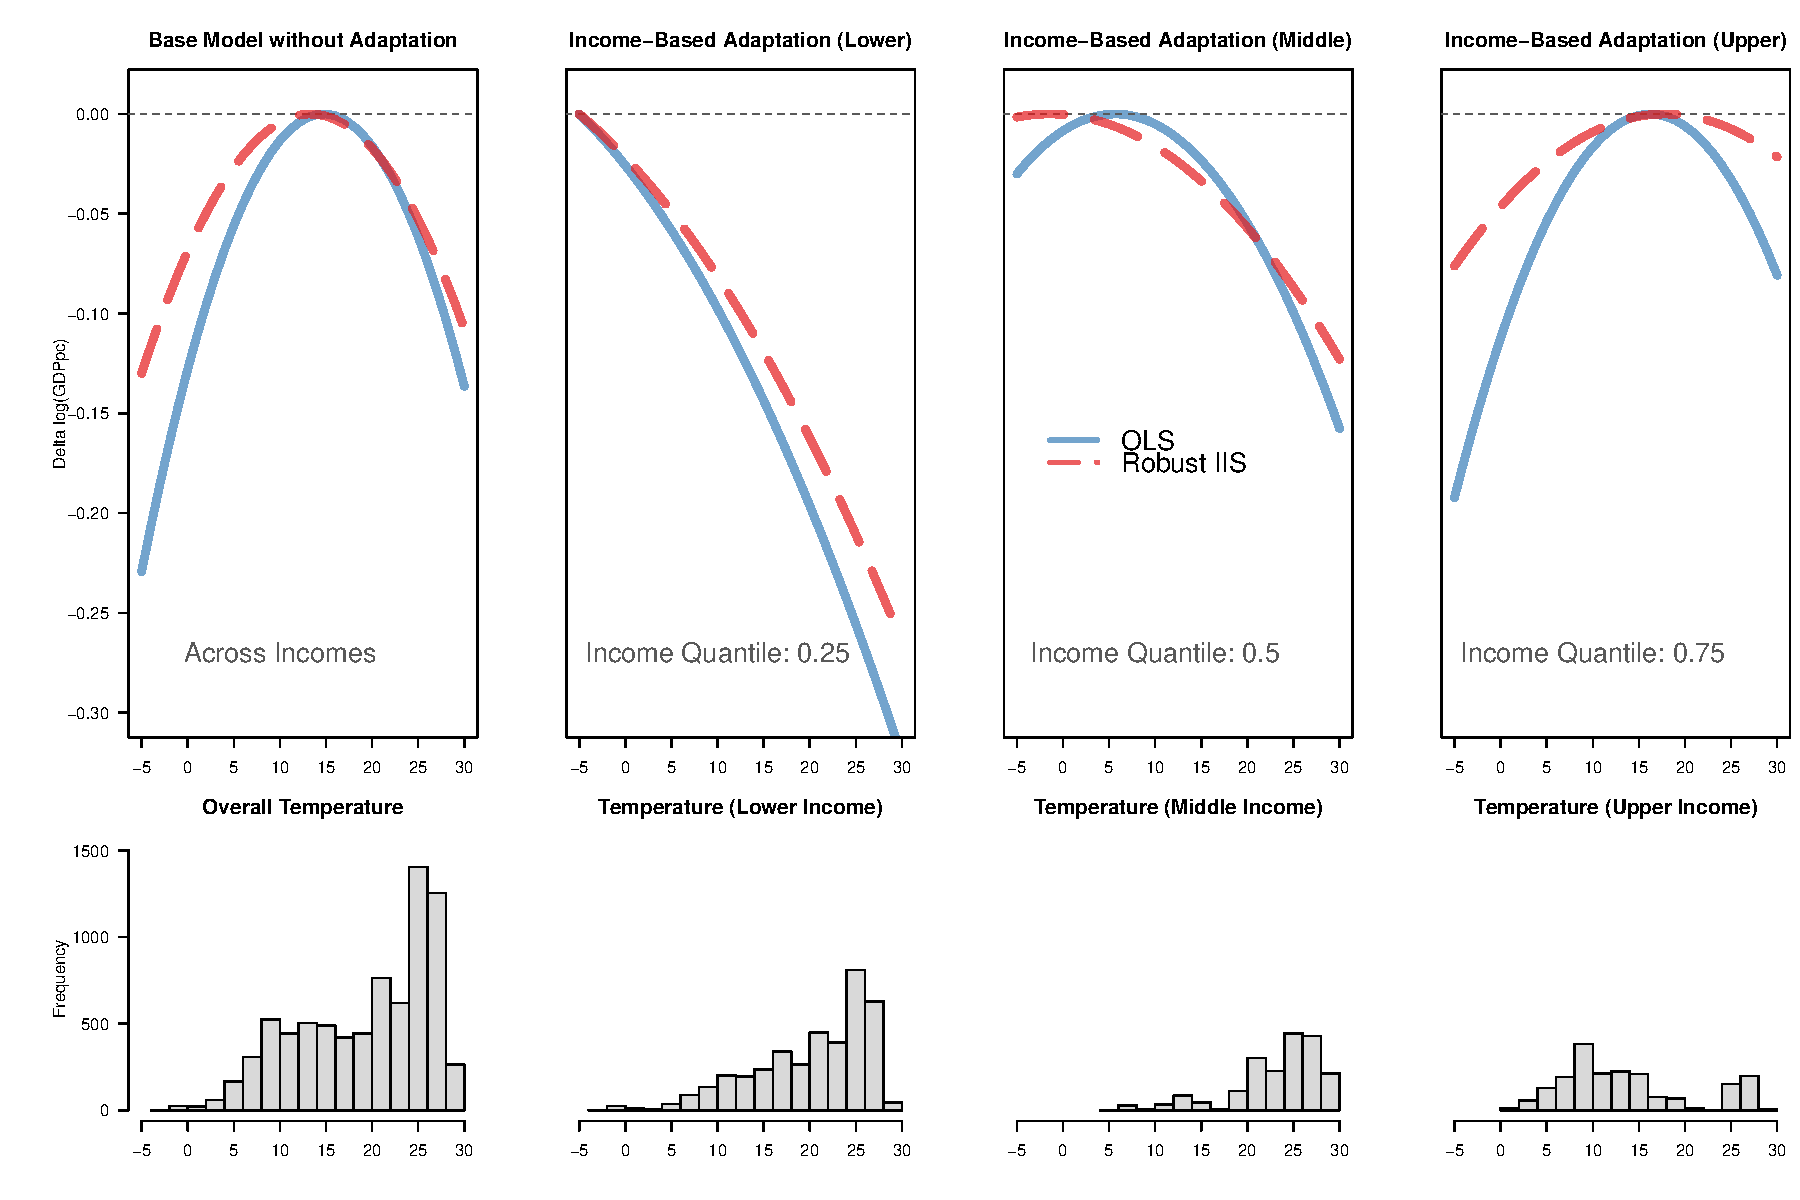
\includegraphics[width = \textwidth]{eff.adapt.v2.pdf}
\caption{Estimated Impact of Temperatures on GDP Per Capita Growth Allowing for Adaptation and Controlling for Outliers. OLS-estimated relationship shown in blue, robust IIS estimated relationship shown in red. Estimated non-linear impact function for the overall base model (top left) and at three different income levels (other top panels). Observed temperatures for the entire sample and across income ranges are shown in the bottom panel. }
\label{fig_dist_app1}
\end{figure}




\begin{figure}[!htbp]  %\vspace{-.35in}
\centering
%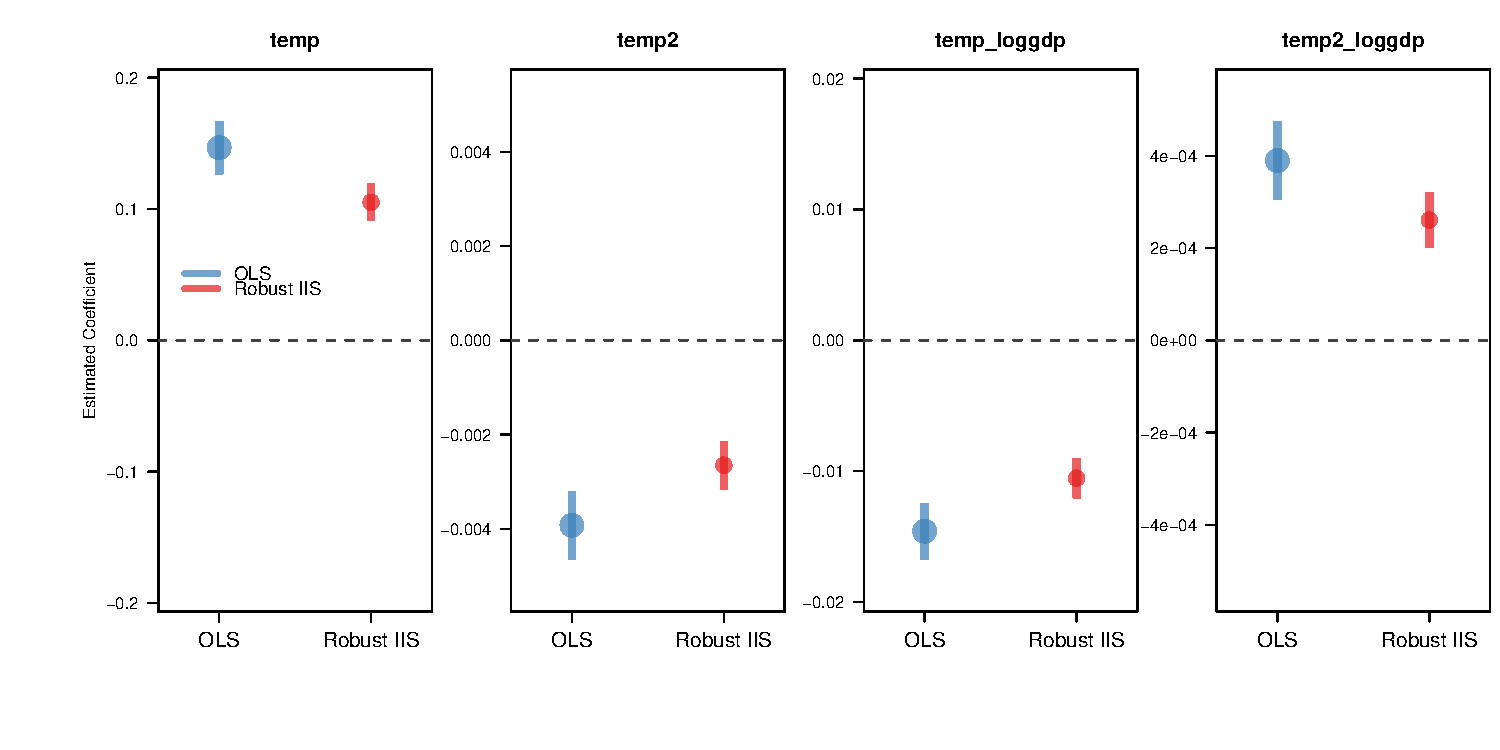
\includegraphics[scale=0.65]{coef_v2_lag.pdf}
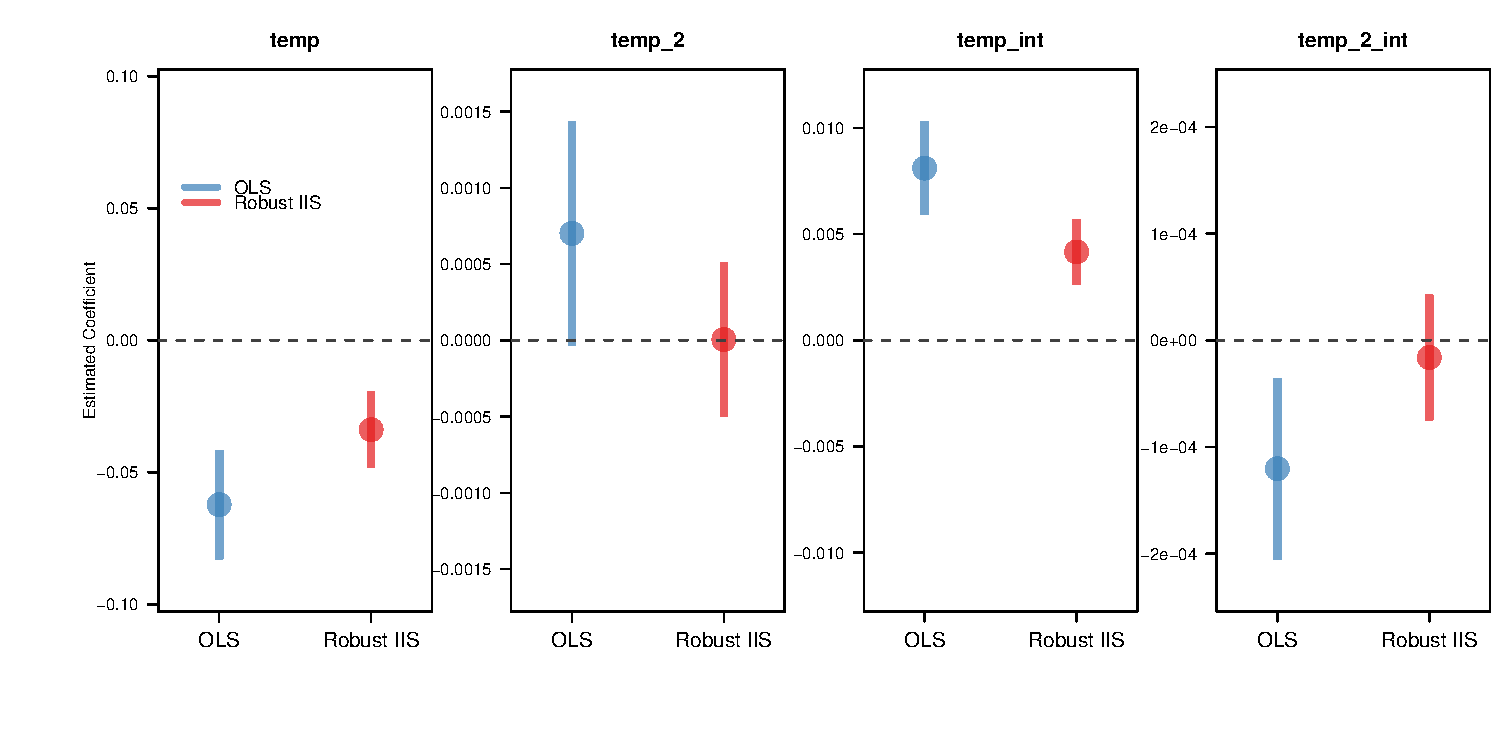
\includegraphics[width = \textwidth]{coef.adapt.pdf}
\caption{Estimated Impact of Temperatures on GDP Per Capita Growth Allowing for Adaptation and Controlling for Outliers. Coefficients on temperatures and the income interaction terms are shown using OLS and the robust IIS estimator. Note that scale of the y-axis differs across plots.}
\label{fig_dist_coef_app1}
\end{figure}

Using these estimates and insights, we project these climate impact estimates to the end of the century by combining gridded temperature estimates from individual CMIP5 model ensemble runs and econometric long-term GDP per capita forecasts from \citet{muller2019econometric}. All our estimates indicate substantial reductions in GDP per capita levels for high levels of warming when compared to our baseline (see Figure \ref{fig_projection} and Table \ref{tab_app2_project}). Base model projections indicate that the median country-level GDP per capita levels could be 63\% lower than the baseline when we aggregate all model estimates beyond 4\textdegree C global mean temperature anomaly to pre-industrial levels (see Table \ref{tab_app2_project}). We find that countries in lower latitudes are most significantly hit.

\begin{figure}[!htbp]  %\vspace{-.35in}
\centering
%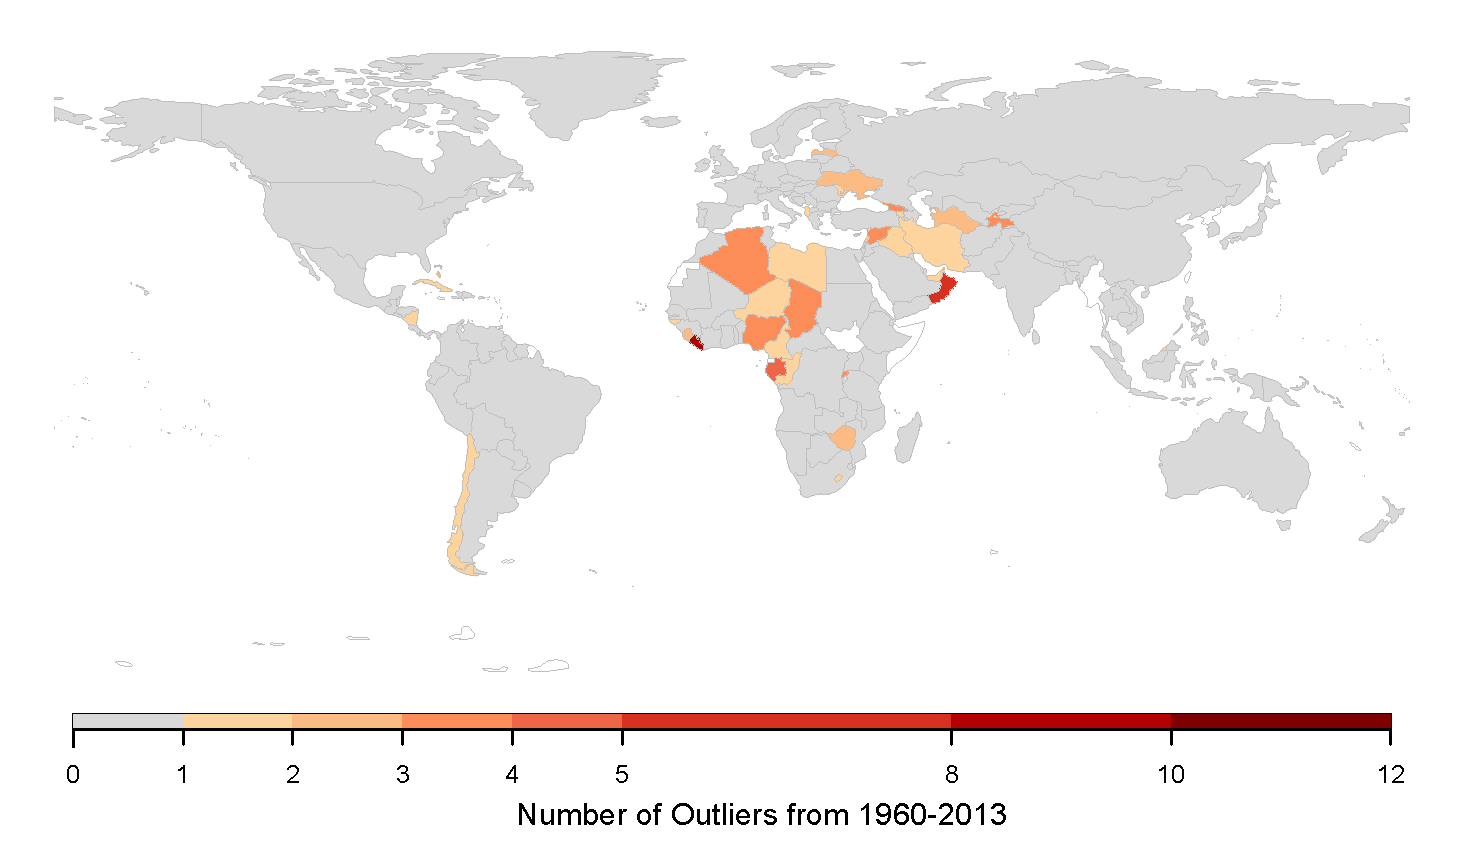
\includegraphics[scale=0.6]{ctry_map_lag_edited.pdf}
\includegraphics[width = \textwidth]{Map_IISBase_noprcp_diff.pdf}
\caption{Projected Climate Impacts for the period 2090 - 2099 and for all CMIP5 models with a mean warming above 4\textdegree C. Projection excludes Precipitation Effect. Estimate shown is the median, grey indicates that the 90\% confidence interval spans 0.}
\label{fig_projection_map}
\end{figure}

Additionally, we consider the influence of income-based adaptation and robust estimation on projections of future climate impacts. Using robust estimates, the projected negative temperature impacts are less steep (but still negative) for low income countries, and dampened for middle income countries. For rich countries, the positive effects of higher temperatures are drastically weakened, suggesting attenuated positive effects -- nonetheless the estimated functional still suggests substantial positive growth effects for countries such as Russia or Mongolia (see bottom panel of Figure \ref{fig_projection_map}). Using robust estimates reduces median country-level GDP per capita impacts by up to 8\% points in our base and adapation model and even up to 13\% points in the adaptation model with lagged adaptation (see Table \ref{tab_app2_project}).

To project estimates of income-based adaptation, we need to project adaptation effects as well. To avoid extrapolation of adaptation out-of-sample we constrain the projected adaptation to the highest in-sample income levels across countries. We further restrict growth impacts under adaptation to not exceed the baseline growth rate where non-adaptation impacts in a particular year would  be negative in our base projections. Further, to reflect that adaptation is a choice, we restrict countries not to be worse-off under adaptation compared to the no-adaptation projection. While these restrictions are theory-motivated and calibrated to the data at hand, such assumptions should be further scrutinised in the future \citet[see ][]{schwarz2020modelling}. When projecting these adaptation results, we find that adapation could plausibly reduce GDP per capita impacts by up to 12\% points under a high warming scenario, highlighting that substantial impacts are to be expected under high warming levels in any case.

Wehn combining both income-adaptation and robust estimation, we additionally identify a change in the marginal rate of impacts with further warming. For a one \textdegree C increase in global mean temperature anomaly from 3\textdegree C to 4\textdegree C, we would expect a 13\% point additional reduction for our OLS base model and a similar reduction for the OLS adaptation model. Using robust estimation and estimates of income-adaptation, however, our results suggest that these additional impacts might be halved to about 5\% per \textdegree C.

Overall, our results provide macro-econometric evidence of income-driven adaptation -- temperatures have a non-linear effect on GDP per capita growth, but this relationship varies by income. Where poor countries face negative impacts of warmer temperatures, rich countries face predominantly positive impacts, with middle-income countries seeing the familiar quadratic relationship (see Figure (\ref{fig_dist_coef_app1}). Moreover, our estimation results highlight the importance of controlling for outlying observations and testing for subsequent distortion. Idiosyncratic shocks in the model distort coefficient estimates, with robust results showing dampened climate impacts onto GDP per capita growth compared to conventional OLS estimates. When considering projections of future climate impacts, our results suggest that both income-adaptation and robust esimation reduces the level of projected climate impacts. When considering both income-adaptation and robust estimation, we further identify a decrease in the marginal rate of impacts with further warming in the adaptation model by about half.

\ignore{Note: Can we show that our residuals produced by IIS are iid normal or at least satisfy either normal, homoscedasticity, or serially independent? Any one of these will help us to defend our paper if referees criticise on our assumptions. In addition, in this case we have a very well specified climate impact model that can pass all the specification tests.}


\begin{figure}[!htbp]  %\vspace{-.35in}
\centering
%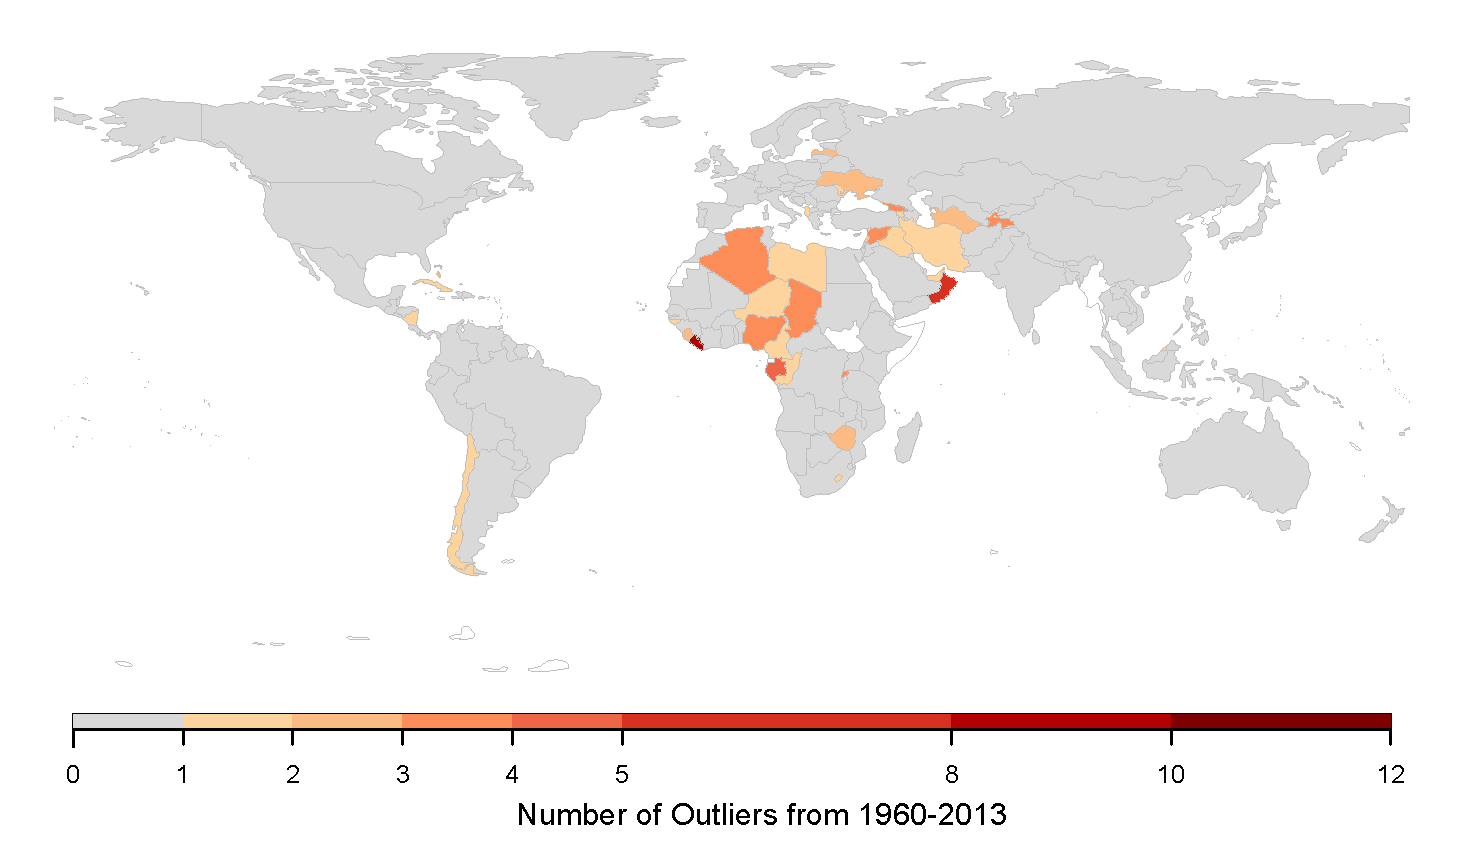
\includegraphics[scale=0.6]{ctry_map_lag_edited.pdf}
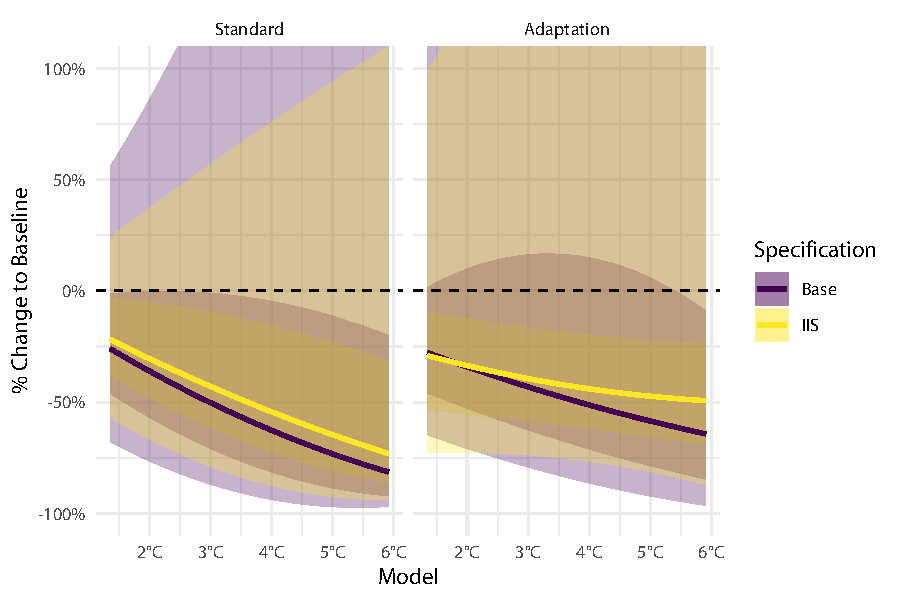
\includegraphics[width = \textwidth]{projections_noprcp_main.pdf}
\caption{Projected Damage Curve for the period 2090 - 2099. Projection excludes Precipitation Effect. Central line is the median. Shadings represent the interquartile range and a 90\% confidence interval.}
\label{fig_projection}
\end{figure}



\begin{table}
\caption{Damage Curve Projection results for all considered models for different levels of Global Mean Temperature Anomaly.}
\label{tab_app2_project}
\centering
\resizebox{\textwidth}{!}{\begin{tabular}[t]{C{3cm}L{5cm}C{2cm}C{2cm}C{3cm}}
\toprule
Global Temperature Anomaly & Model & IIS & OLS & Difference between OLS and IIS\\
\midrule
\addlinespace[0.3em]
\multicolumn{5}{l}{\textbf{}}\\
\hspace{1em}2\textdegree C & Base & -30\% & -36\% & 6\%\\
\hspace{1em}2\textdegree C & Adaptation & -33\% & -34\% & 0\%\\
\hspace{1em}2\textdegree C & Adadptation with Lagged GDP per capita & -24\% & -31\% & 7\%\\
\addlinespace[0.3em]
\multicolumn{5}{l}{\textbf{}}\\
\hspace{1em}3\textdegree C & Base & -43\% & -50\% & 7\%\\
\hspace{1em}3\textdegree C & Adaptation & -39\% & -43\% & 4\%\\
\hspace{1em}3\textdegree C & Adadptation with Lagged GDP per capita & -32\% & -43\% & 10\%\\
\addlinespace[0.3em]
\multicolumn{5}{l}{\textbf{}}\\
\hspace{1em}4\textdegree C & Base & -55\% & -63\% & 8\%\\
\hspace{1em}4\textdegree C & Adaptation & -44\% & -51\% & 7\%\\
\hspace{1em}4\textdegree C & Adadptation with Lagged GDP per capita & -41\% & -54\% & 13\%\\
\bottomrule
\end{tabular}}
\end{table}



\clearpage
\section{Conclusion}
We introduced a formal test to assess outlier distortion in regression models by comparing OLS estimates to those obtained using robust Huber-skip estimators (including Robustified Least Squares and Impulse Indicator Saturation). To develop the proposed test, we fully established asymptotic theory of RLS and IIS. Our analysis is valid in cross sectional and time series settings which include stationary, deterministically trending, and unit root processes. The test performs well in simulations with size close to nominal levels for large ($n>200$) samples and high power under a range of alternatives. Our proposed bootstrap implementation of scaling the cut-off values used to determine outliers improves performance in finite samples and reduces size distortions for the asymptotic test when the reference distribution is different to the true underlying error distribution.

Our application of the outlier distortion test to the macro-economic impacts of climate change highlights the importance of assessing the influence of outliers in regression models. We find that estimates of climate impacts are sensitive to outlying observations that necessitate robust estimation in all model specifications. When using a robust estimator, the estimated impacts of temperatures onto GDP per capita growth are significantly different to those obtained when using OLS as our formal test shows. Our econometric estimates show that temperatures have a non-linear effect on GDP per capita growth, but this relationship varies by income, which is evidence of income-driven adaptation to climate change suggesting that higher incomes dampen the impact that future climate change can have. Resulting projections of impacts with and without adaptation show that robust estimation dampens climate impacts onto GDP per capita growth compared to conventional OLS estimates by up to 8\% in our two central models. When considering income-adaptation in isolation, we project a level reduction of impacts by up to 12\% and when considering both robust estimation and income-adaptation we further find that marginal impacts of an additional degree of warming could roughly halve. Nonetheless, all our projections show that even under adaptation, median estimates of GDP per capita losses could be immense under high levels of warming, reemphasizing the need to achieve the temperature goals of the Paris Agreement to avoid large and significant losses, especially in poor countries.

More generally, our proposed test allows for the assessment of outlier-driven distortion in a wide set of regression models and can be readily implemented using the R-package `gets' (\citealt{pretis2018automated}).

\newpage
\linespread{1} \selectfont
\bibliographystyle{apacite}
\bibliography{outlier_distortion_bib}

%%%%%%%%%%%%%%%%%%%%%%%%%%%%%%%%%%%%%%%%%%%%%%%%%%%%%

\newpage
\appendix
\section{Proofs of The Main Theorems} \label{sec_proofs}
The proofs of the main results proceed as follows: initially the one-step stochastic expansion and tightness results are given for the iterated estimators of $(\beta, \sigma^{2})$ computed from Algorithm \ref{iterated 1-step Huber-skip M-estimator with the same cut-off c}. Next, we show the expansion of the iterated estimators in any step in terms of the initial estimators and establish the fixed point of the iterated estimators upon through infinite iterations. Given the two different type of initial estimators by the Robustified Least Squares and Impulse Indicator Saturation algorithms, we then build up the stochastic expansions of their algorithmic estimators in any iterated step. All these arguments hold uniformly in the cut-off $c \in [c_{+}, \infty)$, so weak convergence theory can be established for the estimators of $(\beta, \sigma^{2})$ seen as stochastic processes in terms of the drifting cut-off $c$. The proof combines the tightness and finite dimensional convergence, showing that the weak limit varies with the stochastic properties of regressors. Finally, we derive the limiting distribution of a new Hausman type test statistics for checking outlier robustness in coefficients.

The updated estimators (\ref{iterated 1-step Huber-skip M-estimator with subscript c}) and (\ref{iterated regression variance estimator with subscript c}) of $(\beta, \sigma^{2})$ involve the weighted and marked empirical processes presented in the following lemma from \cite{jiao2018testing}, which is built on the empirical process theory recently developed by \cite{berenguer2019analysis} (Theorem 4.4). The lemma below is thus to give the first-order asymptotic expansions of the empirical processes appeared in the robust estimators (\ref{iterated 1-step Huber-skip M-estimator with subscript c}) and (\ref{iterated regression variance estimator with subscript c}).

\begin{lemma} \label{asymptotic expansion and tightness of two-sided empirical processes}
(\cite{jiao2018testing}, Lemma 8.2) Suppose Assumption \ref{sufficient assumptions}$(i, iib)$ holds. We have an expansion
\begin{align*}
n^{-1/2} \sum_{i=1}^{n} w_{in} \varepsilon_{i}^{p} 1_{( |\varepsilon_{i} - x_{in}^{\prime}b| \le \sigma c + n^{-1/2} a c )} & = n^{-1/2} \sum_{i=1}^{n} w_{in} \varepsilon_{i}^{p} 1_{(|\varepsilon_{i}| \le \sigma c)} + \mathcal{B}_{n}(a, b, c) + R(a, b, c),
\end{align*}
where the bias term is expressed as
\begin{equation*}
\mathcal{B}_{n}(a, b, c) = 2 \sigma^{p - 1} c^{p} \mathsf{f}(c) n^{-1/2} \sum_{i=1}^{n} w_{in} ( 1_{(p \,\, even)} n^{-1/2} a c  + 1_{(p \,\, odd)} x_{in}^{\prime} b ).
\end{equation*}
Notice $w_{in}$ can be chosen as $1, n^{1/2} x_{in}, n x_{in} x_{in}^{\prime}$ and $p$ as either of $0, 1, 2$. For any $B > 0$ and as $n \to \infty$, the remainder term satisfies
\begin{equation*}
\sup_{0 < c < \infty} \sup_{|a|, |b| \le n^{1/4 - \eta} B} |R(a, b, c)| = \mathrm{o}_{\mathsf{P}}(1).
\end{equation*}
In addition, the normalized process $n^{-1/2} \sum_{i=1}^{n} w_{in} (\varepsilon_{i}^{p} 1_{( |\varepsilon_{i}| \le \sigma c)} - \mathsf{E}_{i - 1} \varepsilon_{i}^{p} 1_{( |\varepsilon_{i}| \le \sigma c)})$ is tight in $c \in \mathbb{R}_{+}$, where $\mathsf{E}_{i - 1}(\cdot) = \mathsf{E}(\cdot | \mathcal{F}_{i - 1})$ and $\mathsf{E}_{i - 1} \varepsilon_{i}^{p} 1_{( |\varepsilon_{i}| \le \sigma c)} = \mathsf{E} \varepsilon_{i}^{p} 1_{( |\varepsilon_{i}| \le \sigma c)} = \sigma^{p} \tau_{p}^{c}$.
\end{lemma}

Before showing the one-step stochastic expansion of the updated estimators, we first present the following lemma, which is a variation of the delta method required for attaining the expansion of $n^{1/2} (\widehat{\sigma}_{c}^{(m + 1)} - \sigma)$ from $n^{1/2} \{ (\widehat{\sigma}_{c}^{(m + 1)})^{2} - \sigma^{2} \}$.

\begin{lemma} \label{variation of delta method}
Let $\{ X_{n} \}$ be a sequence of random variables and $\theta$ be a deterministic parameter. Assume that a univariate function $g$ has the first and second derivatives $\dot{g}, \ddot{g}$, then we have
\begin{equation*}
n^{1/2} \{ g(X_{n}) - g(\theta) \} = \dot{g}(\theta) n^{1/2} (X_{n} - \theta) + n^{-1/2} \ddot{g}(\bar{\theta}) \{ n^{1/2} (X_{n} - \theta) \}^{2},
\end{equation*}
where $|\bar{\theta} - \theta| \le |X_{n} - \theta|$.
\end{lemma}

\begin{proof}[\textnormal{\textbf{Proof of Lemma \ref{variation of delta method}}}]
Approximate $g$ around the point $\theta$ by the linear function using the Taylor expansion and particularly check the approximation at the point $X_{n}$, then
\begin{equation*}
g(X_{n}) = g(\theta) + \dot{g}(\theta) (X_{n} - \theta) + \ddot{g}(\bar{\theta}) (X_{n} - \theta)^{2},
\end{equation*}
where $|\bar{\theta} - \theta| \le |X_{n} - \theta|$. Rearranging the above immediately gives the expansion shown in the lemma.
\end{proof}

Equipped with the empirical processes theory in Lemma \ref{asymptotic expansion and tightness of two-sided empirical processes} and the delta method in Lemma \ref{variation of delta method}, we can now study the updated estimator (\ref{iterated 1-step Huber-skip M-estimator with subscript c}) and (\ref{iterated regression variance estimator with subscript c}) and build up its stochastic expansion in terms of the original estimator, a kernel and a small remainder term. Denote $c_{+} > 0$ as a small positive number.

\begin{lemma} \label{one step expansion of iterated estimators}
Consider the iterated 1-step Huber-skip M-estimator in Algorithm \ref{iterated 1-step Huber-skip M-estimator with the same cut-off c}. Suppose Assumption \ref{sufficient assumptions}$(i, ii)$ holds, and that $N^{-1} (\widehat{\beta}_{c}^{(m)} - \beta)$, $n^{1/2} (\widehat{\sigma}_{c}^{(m)} - \sigma$) are $\mathrm{O}_{\mathsf{P}}(1)$. Then, uniformly in $c \in [c_{+}, \infty)$ and as $n \to \infty$
\begin{align*}
N^{-1} (\widehat{\beta}_{c}^{(m+1)} - \beta) & = \frac{2c\mathsf{f}(c)}{\psi_{c}} N^{-1} (\widehat{\beta}_{c}^{(m)} - \beta) + (\psi_{c} \Sigma_{n})^{-1} \sum_{i=1}^{n} x_{in} \varepsilon_{i} 1_{(|\varepsilon_{i}| \le \sigma c)} + \mathrm{o}_{\mathsf{P}}(1), \\
n^{1/2} (\widehat{\sigma}_{c}^{(m+1)} - \sigma) & = \frac{c(c^{2} - \varsigma_{c}^{2})\mathsf{f}(c)}{\tau_{2}^{c}}n^{1/2} (\widehat{\sigma}_{c}^{(m)} - \sigma) \\
& + \frac{\sigma}{2 \tau_{2}^{c}} n^{-1/2}  \sum_{i=1}^{n} (\frac{\varepsilon_{i}^{2}}{\sigma^{2}} - \varsigma_{c}^{2}) 1_{(|\varepsilon_{i}| \le \sigma c)} + \mathrm{o}_{\mathsf{P}}(1).
\end{align*}
\end{lemma}

\begin{proof}[\textnormal{\textbf{Proof of Lemma \ref{one step expansion of iterated estimators}}}]
The $m+1$ step estimators (\ref{iterated 1-step Huber-skip M-estimator with subscript c}) and (\ref{iterated regression variance estimator with subscript c}) of $\beta$, $\sigma^{2}$ are least squares estimators for the non-outlying observations and satisfy
\begin{align}
    N^{-1} (\widehat{\beta}_{c}^{(m+1)} - \beta)
    & =
    (\sum_{i=1}^{n} x_{in}x_{in}^{\prime} v_{i, c}^{(m)})^{-1}
    (\sum_{i=1}^{n} x_{in}\varepsilon_{i}  v_{i, c}^{(m)}),
    \label{expression for beta in the m+1 step after manipulations}
\\
    n^{1/2} \{ (\widehat{\sigma}_{c}^{(m+1)})^{2} - \sigma^{2} \}
    & =
    \varsigma_{c}^{-2} (n^{-1} \sum_{i=1}^{n} v_{i, c}^{(m)})^{-1}
    n^{-1/2}
    \{
    \sigma^{2} \sum_{i=1}^{n} (\frac{\varepsilon_{i}^{2}}{\sigma^{2}} - \varsigma_{c}^{2}) v_{i, c}^{(m)}
    \label{expression for sigma in the m+1 step after manipulations}
\\
    &
    -
    (\sum_{i=1}^{n} \varepsilon_{i} x_{in}^{\prime} v_{i, c}^{(m)})
    (
    \sum_{i=1}^{n} x_{in} x_{in}^{\prime} v_{i, c}^{(m)}
    )^{-1}
    (\sum_{i=1}^{n} x_{in} \varepsilon_{i} v_{i, c}^{(m)})
    \}.
    \nonumber
\end{align}
We express the weight $v_{i, c}^{(m)}$ in (\ref{iterated 1-step Huber-skip M-indicator with subscript c}) as
\begin{equation} \label{expression for the weight indicators}
v_{i, c}^{(m)} = 1_{(|y_{i} - x_{i}^{\prime} \widehat{\beta}_{c}^{(m)}| \le \widehat{\sigma}_{c}^{(m)} c)} = 1_{(|\varepsilon_{i} - x_{in}^{\prime}\widehat{b}_{c}^{(m)}| \le \sigma c + n^{-1/2} \widehat{a}_{c}^{(m)}c)}, % = v_{i}^{\widehat{a}_{c}^{(m)}, \widehat{b}_{c}^{(m)}, c},
\end{equation}
where $\widehat{b}_{c}^{(m)} = N^{-1} (\widehat{\beta}_{c}^{(m)} - \beta)$ and $\widehat{a}_{c}^{(m)} = n^{1/2} (\widehat{\sigma}_{c}^{(m)} - \sigma)$ are estimation errors for $\beta$ and $\sigma$ in the $m$ step of the algorithm.

By Assumption \ref{sufficient assumptions}$(i, iib)$ and $|\widehat{b}_{c}^{(m)}| + |\widehat{a}_{c}^{(m)}| = \mathrm{O}_{\mathsf{P}}(1)$, we can apply the expansions of the empirical processes in Lemma \ref{asymptotic expansion and tightness of two-sided empirical processes} to (\ref{expression for beta in the m+1 step after manipulations}) and (\ref{expression for sigma in the m+1 step after manipulations}), so for $\widehat{\beta}_{c}^{(m + 1)}$ we have
\begin{equation*}
\widehat{b}_{c}^{(m+1)} = \frac{2c \mathsf{f}(c)}{\psi_{c}} \widehat{b}_{c}^{(m)} + (\psi_{c} \Sigma_{n})^{-1} \sum_{i=1}^{n} x_{in} \varepsilon_{i} 1_{(|\varepsilon_{i}| \le \sigma c)} + R_{\beta}(\widehat{a}_{c}^{(m)}, \widehat{b}_{c}^{(m)}, c),
\end{equation*}
where the remainder $R_{\beta}(a, b, c)$ vanishes uniformly in $c_{+} \le c < \infty$ and $|a|, |b| \le B$. A key to this is that $c$ is bounded away from zero and that $\Sigma_{n} \overset{\mathsf{D}}{\to} \Sigma$ is almost surely positive definite by Assumption \ref{sufficient assumptions}$(iia)$ so that the denominator $\psi_{c}$, $\psi_{c} \Sigma_{n}$ is bounded away from zero.

For $\widehat{\sigma}_{c}^{(m+1)}$, first write $n^{1/2} (\widehat{\sigma}_{c}^{(m + 1)} - \sigma) = n^{1/2} [ \{ (\widehat{\sigma}_{c}^{(m + 1)})^{2} \}^{1/2} - (\sigma^{2})^{1/2} ]$ and let $g(x) = x^{1/2}$, $X_{n} = (\widehat{\sigma}_{c}^{(m + 1)})^{2}$, $\theta = \sigma^{2}$, then apply Lemma \ref{variation of delta method} to obtain
\begin{equation*}
n^{1/2}(\widehat{\sigma}_{c}^{(m+1)} - \sigma) = \frac{1}{2 \sigma} n^{1/2} \{ (\widehat{\sigma}_{c}^{(m+1)})^{2} - \sigma^{2} \} + n^{-1/2} \mathrm{O}[ n \{ (\widehat{\sigma}_{c}^{(m+1)})^{2} - \sigma^{2} \}^{2} ].
\end{equation*}
Notice $\dot{g}(x) = x^{-1/2} / 2$ and $\ddot{g}(x) = - x^{-3/2} / 4$. Next, apply the similar arguments as for $\widehat{\beta}_{c}^{(m + 1)}$ to get
\begin{equation*}
\widehat{a}_{c}^{(m+1)} = \frac{c(c^{2} - \varsigma_{c}^{2})\mathsf{f}(c)}{\tau_{2}^{c}}\widehat{a}_{c}^{(m)} + \frac{\sigma}{2 \tau_{2}^{c}} n^{-1/2}  \sum_{i=1}^{n} (\frac{\varepsilon_{i}^{2}}{\sigma^{2}} - \varsigma_{c}^{2}) 1_{(|\varepsilon_{i}| \le \sigma c)} + R_{\sigma}(\widehat{a}_{c}^{(m)}, \widehat{b}_{c}^{(m)}, c),
\end{equation*}
where the remainder $R_{\sigma}(a, b, c)$ also vanishes uniformly.
\end{proof}

The next step is to prove tightness of iterated estimators. Then, we show the contraction mapping for the one-step expansion of the updated estimator in terms of the original one. With $\eta = 1/4$ corresponding to a bounded initial estimators, this will be sufficient for tightness proof. Note that $|\cdot|$ refers to the usual Euclidean vector norm, while $\| M \| = \max \{ \mathrm{eigen}(M^{\prime}M) \}^{1/2}$ is the spectral norm for any matrix $M$. The norms are compatible so that $|Mx| \le \| M \| |x|$ for any vector $x$.

\begin{proof}[\textnormal{\textbf{Proof of Theorem \ref{tightness of iterated estimators}}}]
To make the proof concise, write the one-step expansion as the compact form
\begin{equation} \label{autoregressive equation for u with 0 remainder term allows the varying cut-off c}
\widehat{u}_{c}^{(m+1)} = \Gamma_{c} \widehat{u}_{c}^{(m)} + K_{c} + R_{u}(\widehat{u}_{c}^{(m)}, c),
\end{equation}
where the remainder term satisfies $\sup_{c_{+} \le c < \infty} \sup_{|u| \le B} |R_{u}(u, c)| = \mathrm{o}_{\mathsf{P}}(1)$ and
\begin{align}
\widehat{u}_{c}^{(m)} & =
                                          \begin{pmatrix}
                                          \widehat{b}_{c}^{(m)} \\
                                          \widehat{a}_{c}^{(m)}
                                          \end{pmatrix}
, \qquad
\Gamma_{c} =
                         \begin{Bmatrix}
                         \frac{2c\mathsf{f}(c)}{\psi_{c}} I_{d_{x}} & 0_{d_{x}} \\
                         0_{d_{x}}^{\prime} & \frac{c(c^{2} - \varsigma_{c}^{2})\mathsf{f}(c)}{\tau_{2}^{c}}
                         \end{Bmatrix}, \label{estimation error u and autoregressive coefficient with the same c}
                         \\
K_{c} & =
               \begin{Bmatrix}
               (\psi_{c} \Sigma_{n})^{-1} & 0_{d_{x}} \\
               0_{d_{x}}^{\prime} & \frac{\sigma}{2 \tau_{2}^{c}}
               \end{Bmatrix}
\sum_{i=1}^{n}
                            \begin{Bmatrix}
                            x_{in} \varepsilon_{i} \\
                            n^{-1/2} (\frac{\varepsilon_{i}^{2}}{\sigma^{2}} - \varsigma_{c}^{2})
                            \end{Bmatrix}
1_{(|\varepsilon_{i}| \le \sigma c)}. \label{kernel with the same c}
\end{align}

Apply the autoregressive equation (\ref{autoregressive equation for u with 0 remainder term allows the varying cut-off c}) recursively to obtain the representation
\begin{equation} \label{recursive representation for u with 0 remainder term allows the varying cut-off c}
\widehat{u}_{c}^{(m+1)} = \Gamma_{c}^{m+1} \widehat{u}_{c}^{(0)} + \sum_{l=0}^{m} \Gamma_{c}^{l} \{ K_{c} + R_{u}(\widehat{u}_{c}^{(m-l)}, c) \}.
\end{equation}
Use the triangle inequality and $|Mx| \le \| M \| |x|$ to get
\begin{equation*}
|\widehat{u}_{c}^{(m+1)}| \le \| \Gamma_{c}^{m+1} \| |\widehat{u}_{c}^{(0)}| + \{ | K_{c} | + \max_{0 \le l \le m} |R_{u}(\widehat{u}_{c}^{(l)}, c)| \} \sum_{l=0}^{m} \| \Gamma_{c}^{l} \|.
\end{equation*}
Assumption \ref{sufficient assumptions}$(i)$ shows $\sup_{c_{+} \le c < \infty} \max \{ |2c\mathsf{f}(c)/\psi_{c}|, |c(c^{2} - \varsigma_{c}^{2})\mathsf{f}(c)/\tau_{2}^{c}| \} < 1$; see Theorem 3.5 in \cite{johansen2013outlier}, so $\sup_{c_{+} \le c < \infty} \| \Gamma_{c} \| < 1$. Thus, by Gelfand's formula, see Theorem 3.4 in \cite{varga2000matrix}, $\lim_{m \to \infty} \| M^{m} \|^{1/m} = \max | \mathrm{eigen}(M) |$, for some $\omega$ such that $\sup_{c_{+} \le c < \infty} \| \Gamma_{c} \| < \omega < 1$ there exists $m_{0} > 0$ so for all $m > m_{0}$ then
\begin{equation} \label{one strong inequality by Gelfand's formula}
\sup_{c_{+} \le c < \infty} \| \Gamma_{c}^{m} \| < \omega^{m} < 1.
\end{equation}
Also note $(I_{d_{x} + 1} - \Gamma_{c})^{-1} = \sum_{l=0}^{\infty} \Gamma_{c}^{l}$. This in turn implies for some $1 < B_{0} < \infty$
\begin{equation} \label{two weak inequalities by Gelfand's formula}
\sup_{0 \le m < \infty} \sup_{c_{+} \le c < \infty} \| \Gamma_{c}^{m} \| < B_{0}, \quad \sup_{c_{+} \le c < \infty} \| (I_{d_{x} + 1} - \Gamma_{c})^{-1} \|  \le \sum_{l=0}^{\infty} \sup_{c_{+} \le c < \infty} \| \Gamma_{c}^{l} \| < B_{0}.
\end{equation}
Therefore, we have for all $m \in [0, \infty)$
\begin{equation} \label{inequality for recursive equation after Gelfand formula}
|\widehat{u}_{c}^{(m+1)}| < B_{0} \{ |\widehat{u}_{c}^{(0)}| + |K_{c}| + \max_{0 \le l \le m} |R_{u}(\widehat{u}_{c}^{(l)}, c)| \}.
\end{equation}
For any $c \in [c_{+}, \infty)$, Assumption \ref{sufficient assumptions}$(iii)$ with $\eta = 1/4$ guarantees tightness of $\widehat{u}_{c}^{(0)}$. Lemma \ref{asymptotic expansion and tightness of two-sided empirical processes} shows that the kernel $K_{c}$ process is tight using Assumption \ref{sufficient assumptions}$(i, iib)$. Thus, for all $\epsilon, \delta > 0$ there exist $n_{0}, U_{0} > 0$ so that for all $n > n_{0}$ the set
\begin{equation} \label{large probability set for tightness and fixed point}
\mathcal{A}_{n} = \{ B_{0} \sup_{c_{+} \le c < \infty} (|\widehat{u}_{c}^{(0)}| + |K_{c}|) \le U_{0}/3, B_{0} \sup_{c_{+} \le c < \infty} \sup_{|u| \le U_{0}} |R_{u}(u, c)| < \delta / 2 \}
\end{equation}
has probability larger than $1 - \epsilon$.

Mathematical induction over $m$ is used to show $\sup_{0 \le m < \infty} \sup_{c_{+} \le c < \infty} |\widehat{u}_{c}^{(m)}| \le U_{0}$ on the set $\mathcal{A}_{n}$. For $m = 0$ as induction starts, $\sup_{c_{+} \le c < \infty} |\widehat{u}_{c}^{(0)}| \le B_{0}^{-1}U_{0}/3 < U_{0}$ holds since $B_{0} > 1$. The induction assumption is that $\sup_{0 \le l \le m} \sup_{c_{+} \le c < \infty} |\widehat{u}_{c}^{(l)}| \le U_{0}$. This implies $B_{0} \max_{0 \le l \le m} |R_{u}(\widehat{u}_{c}^{(l)}, c)| < \delta / 2$, and then the bound in (\ref{inequality for recursive equation after Gelfand formula}) becomes $\sup_{c_{+} \le c < \infty} |\widehat{u}_{c}^{(m+1)}| < 2U_{0}/3 + \delta / 2 < U_{0}$ so that $\sup_{0 \le l \le m+1} \sup_{c_{+} \le c < \infty} |\widehat{u}_{c}^{(l)}| \le U_{0}$.
\end{proof}

Next, we show the expansion of the iterated estimator from Algorithm \ref{iterated 1-step Huber-skip M-estimator with the same cut-off c} at any step in terms of its starting point.

\begin{proof}[\textnormal{\textbf{Proof of Theorem \ref{general expansion in terms of initial estimators}}}]
Directly apply the recursive representation (\ref{recursive representation for u with 0 remainder term allows the varying cut-off c}) in the tightness proof, so uniformly in $c \in [c_{+}, \infty)$ and for any $m \in [0, \infty)$
\begin{equation*}
\widehat{u}_{c}^{(m + 1)} = \Gamma_{c}^{m + 1} \widehat{u}_{c}^{(0)} + \sum_{l = 0}^{m} \Gamma_{c}^{l} K_{c} + \sum_{l = 0}^{m} \Gamma_{c}^{l} R_{u}(\widehat{u}_{c}^{(m - l)}, c),
\end{equation*}
where $\sup_{c_{+} \le c < \infty} \sup_{|u| \le B} |R_{u}(u, c)| = \mathrm{o}_{\mathsf{P}}(1)$. Since the spectral radius of $\Gamma_{c}$ is bounded by one, see (\ref{one strong inequality by Gelfand's formula}), then (\ref{two weak inequalities by Gelfand's formula}) shows for $1 < B_{0} < \infty$
\begin{equation*}
\sup_{c_{+} \le c < \infty} \| \sum_{l = 0}^{m} \Gamma_{c}^{l} \| \le \sup_{c_{+} \le c < \infty} \sum_{l = 0}^{m} \| \Gamma_{c}^{l} \| \le \sum_{l = 0}^{\infty} \sup_{c_{+} \le c < \infty} \| \Gamma_{c}^{l} \| < B_{0}.
\end{equation*}
Further with tightness $\sup_{0 \le m < \infty} \sup_{c_{+} \le c < \infty} |\widehat{u}_{c}^{(m)}| = \mathrm{O}_{\mathsf{P}}(1)$ shown in Theorem \ref{tightness of iterated estimators} due to Assumption \ref{sufficient assumptions} with $\eta = 1/4$, the third term vanishes in the above recursive representation. Applying the equality
\begin{equation} \label{finite sum of geometric matrix sequence}
\sum_{l = 0}^{m} \Gamma_{c}^{l} = (I_{d_{x} + 1} - \Gamma_{c})^{-1} (I_{d_{x} + 1} - \Gamma_{c}^{m+1}) = (I_{d_{x} + 1} - \Gamma_{c}^{m+1}) (I_{d_{x} + 1} - \Gamma_{c})^{-1},
\end{equation}
we then rearrange the recursive representation to attain
\begin{equation} \label{m+1 step stochastic expansion in terms of initial estimators, kernels, and small remainder terms}
\widehat{u}_{c}^{(m + 1)} = \Gamma_{c}^{m + 1} \widehat{u}_{c}^{(0)} + (I_{d_{x} + 1} - \Gamma_{c}^{m + 1}) (I_{d_{x} + 1} - \Gamma_{c})^{-1} K_{c} + \mathrm{o}_{\mathsf{P}}(1),
\end{equation}
uniformly in $c, m$. Recall the definition of $\Gamma_{c}$ in (\ref{estimation error u and autoregressive coefficient with the same c}), then
\begin{align*}
\Gamma_{c}^{m + 1} & =
\begin{bmatrix}
\{ \frac{2 c \mathsf{f}(c)}{\psi_{c}} \}^{m + 1} I_{d_{x}} & 0_{d_{x}} \\
0_{d_{x}}^{\prime} & \{ \frac{c (c^{2} - \varsigma^{2}_{c}) \mathsf{f}(c)}{\tau_{2}^{c}} \}^{m + 1}
\end{bmatrix}
,
\\
(I_{d_{x}+ 1} - \Gamma_{c}^{m + 1}) (I_{d_{x} + 1} - \Gamma_{c})^{-1} & =
\begin{bmatrix}
\frac{\psi_{c}^{m + 1} - \{ 2 c \mathsf{f}(c) \}^{m + 1}}{\psi_{c}^{m} \{ \psi_{c} - 2 c \mathsf{f}(c) \}} I_{d_{x}} & 0_{d_{x}} \\
0_{d_{x}}^{\prime} & \frac{(\tau_{2}^{c})^{m + 1} - \{ c (c^{2} - \varsigma_{c}^{2}) \mathsf{f}(c) \}^{m + 1}}{(\tau_{2}^{c})^{m} \{ \tau_{2}^{c} - c (c^{2} - \varsigma_{c}^{2}) \mathsf{f}(c) \}}
\end{bmatrix}
.
\end{align*}
Finally, substitute these and $\widehat{u}_{c}^{(0)}$, $K_{c}$ into (\ref{m+1 step stochastic expansion in terms of initial estimators, kernels, and small remainder terms}) to establish the expansion of $\widehat{u}_{c}^{(m + 1)}$; see $\widehat{u}_{c}^{(0)}$ in (\ref{estimation error u and autoregressive coefficient with the same c}) and $K_{c}$ in (\ref{kernel with the same c}).
\end{proof}

The next corollary re-expresses Lemma \ref{one step expansion of iterated estimators} as a stochastic expansion of the fist step estimators in terms of the initial ones, which is a special case of Theorem \ref{general expansion in terms of initial estimators} where $m = 0$.

\begin{proof}[\textnormal{\textbf{Proof of Corollary \ref{expansion of the first step estimators}}}]
The proof follows by setting $m = 0$ in Theorem \ref{general expansion in terms of initial estimators} where $\varrho_{\beta, c}^{(1)} = 2 c \mathsf{f}(c) / \psi_{c}$, $\varrho_{x \varepsilon, c}^{(1)}  = \psi_{c}^{-1}$, $\varrho_{\sigma, c}^{(1)} = c (c^{2} - \varsigma_{c}^{2}) \mathsf{f}(c) / \tau_{2}^{c}$, and $\varrho_{\varepsilon \varepsilon, c}^{(1)} = \sigma / (2 \tau_{2}^{c})$.
\end{proof}

We then establish the fixed point of the iterated one-step Huber-skip M-estimators defined in Algorithm \ref{iterated 1-step Huber-skip M-estimator with the same cut-off c}.

\begin{proof}[\textnormal{\textbf{Proof of Theorem \ref{fixed point of iterated estimators}}}]
Since the spectral radius of $\Gamma_{c}$ is strictly smaller than one, see (\ref{one strong inequality by Gelfand's formula}), we have $\Gamma_{c}^{m + 1} \to 0_{(d_{x} + 1) \times (d_{x} + 1)}$ uniformly in $c \in [c_{+}, \infty)$ as $m \to \infty$. Further with the boundedness of $\widehat{u}_{c}^{(0)}$ in probability as $n \to \infty$ by Assumption \ref{sufficient assumptions}$(iii)$ with $\eta = 1/4$, the first term in (\ref{m+1 step stochastic expansion in terms of initial estimators, kernels, and small remainder terms}) vanishes. Notice that to attain the recursive representation (\ref{m+1 step stochastic expansion in terms of initial estimators, kernels, and small remainder terms}) in the proof of Theorem \ref{general expansion in terms of initial estimators}, we also require Assumption \ref{sufficient assumptions}$(i, ii)$. Thus, let $n, m \to \infty$ in (\ref{m+1 step stochastic expansion in terms of initial estimators, kernels, and small remainder terms}), we can then obtain the fixed point
\begin{equation} \label{fixed point for theta with the varying cut-off c}
\widehat{u}_{c}^{(\ast)} = \widehat{u}_{c}^{(\infty)} = (I_{d_{x} + 1} - \Gamma_{c})^{-1} K_{c},
\end{equation}
uniformly in $c$. Recall the definition of $\Gamma_{c}$ in (\ref{estimation error u and autoregressive coefficient with the same c}), we then have
\begin{equation*}
(I_{d_{x} + 1} - \Gamma_{c})^{-1} =
\begin{Bmatrix}
\frac{\psi_{c}}{\psi_{c} - 2 c \mathsf{f}(c)} I_{d_{x}} & 0_{d_{x}} \\
0_{d_{x}}^{\prime} & \frac{\tau_{2}^{c}}{\tau_{2}^{c} - c (c^{2} - \varsigma_{c}^{2}) \mathsf{f}(c)}
\end{Bmatrix}
.
\end{equation*}
Substitute this and $K_{c}$ into (\ref{fixed point for theta with the varying cut-off c}) to attain the expression of the fixed point $\widehat{u}_{c}^{(\ast)}$; see $K_{c}$ in (\ref{kernel with the same c}).

% Based on Assumption \ref{sufficient assumptions}, Theorem \ref{1-step stochastic expansion allows varying cut-off c for the iterated 1-step Huber-skip M-estimator} provides the 1-step equation (\ref{autoregressive equation for u with 0 remainder term allows the varying cut-off c}). Then Theorem \ref{tightness allows varying cut-off c for the iterated 1-step Huber-skip M-estimator} shows $\sup_{0 \le m < \infty} \sup_{c_{+} \le c < \infty} |\widehat{u}_{c}^{(m)}| = \mathrm{O}_{\mathsf{P}}(1)$, so the remainder term in (\ref{autoregressive equation for u with 0 remainder term allows the varying cut-off c}) is $\mathrm{o}_{\mathsf{P}}(1)$. Thus, for $m, n \to \infty$ the fixed point should satisfy $\widehat{u}_{c}^{(\ast)} = \Gamma_{c} \widehat{u}_{c}^{(\ast)} + K_{c}$ so that
% \begin{equation} \label{fixed point for u with the varying cut-off c}
% \widehat{u}_{c}^{(\ast)} = (I_{d_{x} + 1} - \Gamma_{c})^{-1} K_{c}.
% \end{equation}
% Substitute (\ref{estimation error u and autoregressive coefficient with the same c}), (\ref{kernel with the same c}) of $\widehat{u}_{c}^{(\ast)}$, $\Gamma_{c}$ and $K_{c}$ into (\ref{fixed point for u with the varying cut-off c}) to obtain
% \begin{equation*}
 % \begin{Bmatrix}
 % N^{-1} (\widehat{\beta}_{c}^{(\ast)} - \beta) \\
 % n^{1/2} (\widehat{\sigma}_{c}^{(\ast)} - \sigma)
 % end{Bmatrix}
% =
%  \begin{bmatrix}
%   \frac{1}{\psi_{c} - 2c\mathsf{f}(c)} \Sigma^{-1} \sum_{i=1}^{n} N^{\prime} x_{i} \varepsilon_{i} 1_{(|\varepsilon_{i}| \le \sigma c)} \\
%  \frac{1}{2 \sigma \{ \tau_{2}^{c} - c(c^{2} - \varsigma_{c}^{2})\mathsf{f}(c) \}} n^{-1/2} \sum_{i=1}^{n} (\varepsilon_{i}^{2} - \varsigma_{c}^{2} \sigma^{2}) 1_{(|\varepsilon_{i}| \le \sigma c)}
%   \end{bmatrix}
% .
% \end{equation*}

The next step is to formally prove that $\widehat{u}_{c}^{(\ast)}$ is indeed the fixed point. Replace (\ref{recursive representation for u with 0 remainder term allows the varying cut-off c}) and (\ref{fixed point for theta with the varying cut-off c}) into the deviation $\widehat{\Delta}_{c}^{(m+1)} = \widehat{u}_{c}^{(m+1)} - \widehat{u}_{c}^{(\ast)}$ and apply (\ref{finite sum of geometric matrix sequence}) to attain
\begin{equation*}
\widehat{\Delta}_{c}^{(m+1)} = \Gamma_{c}^{m+1} \{ \widehat{u}_{c}^{(0)} - (I_{d_{x} + 1} - \Gamma_{c})^{-1}K_{c} \} + \sum_{l=0}^{m} \Gamma_{c}^{l} R_{u}(\widehat{u}_{c}^{(m-l)}, c).
\end{equation*}
To bound $\widehat{\Delta}_{c}^{(m+1)}$, use the triangle inequality and $|M x| \le \| M \| |x|$ to get
\begin{equation*}
|\widehat{\Delta}_{c}^{(m+1)}| \le \| \Gamma_{c}^{m+1} \| \{ |\widehat{u}_{c}^{(0)}| + \| (I_{d_{x} + 1} - \Gamma_{c})^{-1} \| |K_{c}| \} + \max_{0 \le l \le m} |R_{u}(\widehat{u}_{c}^{(l)}, c)| \sum_{l=0}^{m} \| \Gamma_{c}^{l} \|.
\end{equation*}
Further bound above using the inequalities (\ref{one strong inequality by Gelfand's formula}) and (\ref{two weak inequalities by Gelfand's formula}), so for $m > m_{0}$
\begin{equation*}
|\widehat{\Delta}_{c}^{(m+1)}| < \omega^{m+1} ( |\widehat{u}_{c}^{(0)}| + B_{0} |K_{c}| ) + B_{0} \max_{0 \le l \le m} |R_{u}(\widehat{u}_{c}^{(l)}, c)|.
\end{equation*}
On the set $\mathcal{A}_{n}$ as in (\ref{large probability set for tightness and fixed point}), since $\sup_{0 \le m < \infty} \sup_{c_{+} \le c < \infty} |\widehat{u}_{c}^{(m)}| \le U_{0}$ by Theorem \ref{tightness of iterated estimators}, then $\sup_{c_{+} \le c < \infty} |\widehat{\Delta}_{c}^{(m+1)}| < \omega^{m+1}(B_{0}^{-1}U_{0}/3 + U_{0}/3) + \delta / 2 < \omega^{m+1}U_{0} + \delta / 2$. As $0 < \omega < 1$, $\omega^{m+1}$ declines exponentially so $m_{0}$ can be chosen sufficiently large that for all $m > m_{0}$ then $\omega^{m+1}U_{0} < \delta / 2$. Thus, $\mathsf{P} (\sup_{c_{+} \le c < \infty} |\widehat{\Delta}_{c}^{(m+1)}| < \delta) > 1 - \epsilon$ for $m > m_{0}$, $n > n_{0}$.
\end{proof}

Next considering RLS and IIS, we first build up their stochastic expansions.

\begin{proof}[\textnormal{\textbf{Proof of Theorem \ref{general expansion for RLS and IIS}}}]
We first establish the expansion for the Robustified Least Squares. Then, we show that the Impulse Indicator Saturation has the identical expansion of the initial step updated estimator as the Robustified Least Squares so that they have the same general $m + 1$ step expansion for any $m \in [0, \infty)$.

RLS starts with the full sample least squares $(\widetilde{\beta}, \widetilde{\sigma})$ which are tight and satisfy
\begin{align*}
N^{-1} (\widetilde{\beta} - \beta) & = (\sum_{i = 1}^{n} x_{in} x_{in}^{\prime})^{-1} (\sum_{i = 1}^{n} x_{in} \varepsilon_{i}), \\
n^{1/2} (\widetilde{\sigma} - \sigma) & = \frac{\sigma}{2} n^{-1/2} \sum_{i = 1}^{n} (\frac{\varepsilon_{i}^{2}}{\sigma^{2}} - 1) +  \mathrm{O}_{\mathsf{P}}(n^{-1/2}).
\end{align*}
Substitute the above expansion of the initial estimators $(\widehat{\beta}_{c}^{(0)}, \widehat{\sigma}_{c}^{(0)}) = (\widetilde{\beta}, \widetilde{\sigma})$ into Theorem \ref{general expansion in terms of initial estimators} using Assumption \ref{sufficient assumptions}$(i, ii)$, then it holds for any $m \in [0, \infty)$,
\begin{align*}
N^{-1} (\widehat{\beta}_{c}^{(m + 1)} - \beta) & = \varrho_{\beta, c}^{(m + 1)} \Sigma_{n}^{-1} \sum_{i = 1}^{n} x_{in} \varepsilon_{i} + \varrho_{x \varepsilon, c}^{(m + 1)} \Sigma_{n}^{-1} \sum_{i = 1}^{n} x_{in} \varepsilon_{i} 1_{(|\varepsilon_{i}| \le \sigma c)} +  \mathrm{o}_{\mathsf{P}}(1), \\
n^{1/2} (\widehat{\sigma}_{c}^{(m + 1)} - \sigma) & = \varrho_{\sigma, c}^{(m + 1)} \frac{\sigma}{2} n^{-1/2} \sum_{i = 1}^{n} (\frac{\varepsilon_{i}^{2}}{\sigma^{2}} - 1) \\
& + \varrho_{\varepsilon \varepsilon, c}^{(m + 1)} n^{-1/2} \sum_{i=1}^{n} (\frac{\varepsilon_{i}^{2}}{\sigma^{2}} - \varsigma_{c}^{2}) 1_{(|\varepsilon_{i}| \le \sigma c)} +  \mathrm{o}_{\mathsf{P}}(1),
\end{align*}
uniformly in $c \in [c_{+}, \infty)$.

To demonstrate that two algorithms RLS and IIS have the identical expansion of $N^{-1} (\widehat{\beta}_{c}^{(m + 1)} - \beta)$ for $m \in [0, \infty)$ even they start with different initial estimators when running Algorithm \ref{iterated 1-step Huber-skip M-estimator with the same cut-off c}, it suffices to show that the expansion of $N^{-1} (\widehat{\beta}_{c}^{(1)} - \beta)$ for IIS is the same as RLS in the above. The updated estimator for $\beta$ from an initial step in IIS is expressed as
\begin{align*}
N^{-1} (\widehat{\beta}_{c}^{(1)} - \beta) & = \{ \sum_{j = 1, 2} (N_{3 - j}^{-1} N)^{\prime} \sum_{i \in \mathcal{I}_{3 - j}} x_{i n_{3 - j}} x_{i n_{3 - j}}^{\prime} 1_{(|y_{i} - x_{i}^{\prime} \widehat{\beta}_{j}| \le \widehat{\sigma}_{j} c)} N_{3 - j}^{-1} N \}^{-1} \\
& \times \{ \sum_{j = 1, 2} (N_{3 - j}^{-1} N)^{\prime} \sum_{i \in \mathcal{I}_{3 - j}} x_{i n_{3 - j}} \varepsilon_{i} 1_{(|y_{i} - x_{i}^{\prime} \widehat{\beta}_{j}| \le \widehat{\sigma}_{j} c)} \}.
\end{align*}
Notice $x_{i n_{j}} = N^{\prime}_{j} x_{i}$ denotes the normalized regressors for each subsample $i \in \mathcal{I}_{j}$, $j = 1, 2$, where $N_{j}$ corresponds to the normalization matrix based on the subsample size $n_{j}$.
Argue along the lines of Lemma \ref{one step expansion of iterated estimators} using the expansions in Lemma \ref{asymptotic expansion and tightness of two-sided empirical processes}, then it follows
\begin{align*}
N^{-1} (\widehat{\beta}_{c}^{(1)} - \beta) & = (\psi_{c} \Sigma_{n})^{-1} \{ 2 c \mathsf{f}(c) \sum_{j = 1, 2} (N_{3 - j}^{-1} N)^{\prime} \Sigma_{n_{3 - j}}^{\mathcal{I}_{3 - j}} (N_{3 - j}^{-1} N_{j}) N_{j}^{-1} (\widehat{\beta}_{j} - \beta) \\
& + \sum_{i = 1}^{n} x_{i n} \varepsilon_{i} 1_{(|\varepsilon_{i}| \le \sigma c)} \} + \mathrm{o}_{\mathsf{P}}(1),
\end{align*}
uniformly in $c \in [c_{+}, \infty)$ and where we denote $\Sigma_{n_{j}}^{\mathcal{I}_{j}} = \sum_{i \in \mathcal{I}_{j}} x_{i n_{j}} x_{i n_{j}}^{\prime}$ for $j = 1, 2$. To apply the empirical processes argument in the above, we require Assumption \ref{sufficient assumptions}$(i, iib)$ holding for each subsample $\mathcal{I}_{j}$ and the fact that the initial estimators $N_{j}^{-1} (\widehat{\beta}_{j} - \beta)$, $n_{j}^{1/2} (\widehat{\sigma}_{j} - \sigma)$ are tight for $j = 1, 2$. Further substituting the expansion of least squares on each subsample $\mathcal{I}_{j}$, that is $N_{j}^{-1} (\widehat{\beta}_{j} - \beta) = (\Sigma_{n_{j}}^{\mathcal{I}_{j}})^{-1} \sum_{i \in \mathcal{I}_{j}} x_{i n_{j}} \varepsilon_{i}$ for $j = 1, 2$, we have
\begin{align*}
N^{-1} (\widehat{\beta}_{c}^{(1)} - \beta) & = \frac{2 c \mathsf{f}(c)}{\psi_{c}} \Sigma_{n}^{-1} \sum_{j = 1, 2} (N_{3 - j}^{-1} N)^{\prime} \Sigma_{n_{3 - j}}^{\mathcal{I}_{3 - j}} (N_{3 - j}^{-1} N_{j}) (\Sigma_{n_{j}}^{\mathcal{I}_{j}})^{-1} \sum_{i \in \mathcal{I}_{j}} x_{in_{j}} \varepsilon_{i} \\
& + (\psi_{c} \Sigma_{n})^{-1} \sum_{i = 1}^{n} x_{in} \varepsilon_{i} 1_{(|\varepsilon_{i}| \le \sigma c)} + \mathrm{o}_{\mathsf{P}}(1).
\end{align*}
Notice that we assume $n_{1} = \mathrm{int}[n / 2]$ and $n_{2} = n - n_{1}$ so that $N_{3 - j}^{-1} N_{j} \to I_{d_{x}}$ and $N_{j} N_{3 - j}^{-1} \to I_{d_{x}}$ as $n \to \infty$ and $n_{j} \to \infty$ for $j = 1, 2$. Combine this fact and Assumption \ref{sufficient assumptions}$(iia)$ that $\Sigma_{n_{j}}^{\mathcal{I}_{j}} \overset{\mathsf{P}}{\to} \Sigma$ for $j = 1, 2$ to attain
\begin{equation*}
N^{-1} (\widehat{\beta}_{c}^{(1)} - \beta) = \frac{2 c \mathsf{f}(c)}{\psi_{c}} \Sigma_{n}^{-1} \sum_{i = 1}^{n} x_{in} \varepsilon_{i} + (\psi_{c} \Sigma_{n})^{-1} \sum_{i = 1}^{n} x_{in} \varepsilon_{i} 1_{(|\varepsilon_{i}| \le \sigma c)} + \mathrm{o}_{\mathsf{P}}(1).
\end{equation*}
Then, we find that RLS and IIS have the identical expansion of $N^{-1} (\widehat{\beta}_{c}^{(1)} - \beta)$ by noting $\varrho_{\beta, c}^{(1)} = 2 c \mathsf{f}(c) / \psi_{c}$ and $\varrho_{x \varepsilon, c}^{(1)} = \psi_{c}^{-1}$, so as for the general $m + 1$ step beta estimators for $m \in [0, \infty)$. Using the similar reasoning as on beta, it follows that two algorithms also have the same expansion on sigma.
\end{proof}

Drifting the cut-off value $c \in [c_{+}, \infty)$, we derive the weak convergence theory of the processes $\mathbb{G}_{n}^{(m + 1)}(c) = N^{-1} (\widehat{\beta}_{c}^{(m + 1)} - \beta)$ computed by RLS and IIS for any $m \in [0, \infty)$ in the stationary case, where $N = n^{-1/2} I_{d_{x}}$ such that $x_{in} = n^{-1/2} x_{i}$ and $\Sigma = \mathsf{E} x_{i} x_{i}^{\prime}$.

\begin{proof}[\textnormal{\textbf{Proof of Theorem \ref{weak convergence for RLS and IIS}}}]
By Assumption \ref{sufficient assumptions}$(i, ii)$, Theorem \ref{general expansion for RLS and IIS}
shows that for any $m \in [0, \infty)$ and uniformly in $c \in [c_{+}, \infty)$
\begin{equation*}
\mathbb{G}_{n}^{(m + 1)}(c) =
\begin{pmatrix}
\varrho_{\beta, c}^{(m + 1)} \Sigma_{n}^{-1} \\
\varrho_{x \varepsilon, c}^{(m + 1)} \Sigma_{n}^{-1}
\end{pmatrix}^{\prime}
\sum_{i = 1}^{n}
\begin{pmatrix}
x_{in} \varepsilon_{i} \\
x_{in} \varepsilon_{i} 1_{(|\varepsilon_{i}| \le \sigma c)}
\end{pmatrix}
+ \mathrm{o}_{\mathsf{P}}(1).
\end{equation*}
Then, by $\Sigma_{n} \overset{\mathsf{P}}{\to} \Sigma > 0$, the limiting distribution of the kernel vector, and Slutsky's theorem, we have for any $c \in [c_{+}, \infty)$
\begin{equation*}
\mathbb{G}_{n}^{(m + 1)}(c) \overset{\mathsf{D}}{\to}
\begin{pmatrix}
\varrho_{\beta, c}^{(m + 1)} \Sigma^{-1} \\
\varrho_{x \varepsilon, c}^{(m + 1)} \Sigma^{-1}
\end{pmatrix}^{\prime}
\mathsf{N}
\begin{Bmatrix}
\begin{pmatrix}
0_{d_{x}} \\
0_{d_{x}}
\end{pmatrix}
,
\sigma^{2} \tau_{2}^{c}
\begin{pmatrix}
\frac{1}{\tau_{2}^{c}} \Sigma & \Sigma \\
\Sigma & \Sigma
\end{pmatrix}
\end{Bmatrix}.
\end{equation*}
Since a transformation of multivariate normal is still normal, it follows
\begin{equation*}
\mathbb{G}_{n}^{(m + 1)}(c) \overset{\mathsf{D}}{\to} \mathsf{N} [0_{d_{x}}, \{ (\varrho_{\beta, c}^{(m + 1)})^{2} + 2 \tau_{2}^{c} \varrho_{\beta, c}^{(m + 1)} \varrho_{x \varepsilon, c}^{(m + 1)} + \tau_{2}^{c} (\varrho_{x \varepsilon, c}^{(m + 1)})^{2} \} \sigma^{2} \Sigma^{-1}].
\end{equation*}
Theorem \ref{tightness of iterated estimators} demonstrates the tightness of the processes $\mathbb{G}_{n}^{(m + 1)}$ for any $m \in [0, \infty)$, so
\begin{equation*}
\mathbb{G}_{n}^{(m + 1)} \leadsto \mathbb{G}^{(m + 1)},
\end{equation*}
where the weak limit $\mathbb{G}^{(m + 1)}$ is a zero mean Gaussian process with the variance
\begin{equation*}
\mathsf{Var} \{ \mathbb{G}^{(m + 1)}(c) \} = \{ (\varrho_{\beta, c}^{(m + 1)})^{2} + 2 \tau_{2}^{c} \varrho_{\beta, c}^{(m + 1)} \varrho_{x \varepsilon, c}^{(m + 1)} + \tau_{2}^{c} (\varrho_{x \varepsilon, c}^{(m + 1)})^{2} \} \sigma^{2} \Sigma^{-1}. \qedhere
\end{equation*}
\end{proof}

Next, we give the weak convergence of the first step and fixed point estimator of RLS and IIS.

\begin{proof}[\textnormal{\textbf{Proof of Corollary \ref{weak convergence for the first step and fixed point of RLS and IIS}}}]
These are two special cases of Theorem \ref{weak convergence for RLS and IIS} where $m = 0$ such that $\varrho_{\beta, c}^{(1)} = 2 c \mathsf{f}(c) / \psi_{c}$, $\varrho_{x \varepsilon, c}^{(1)} = \psi_{c}^{-1}$ and where $m \to \infty$ such that $\varrho_{\beta, c}^{(\infty)} = 0$, $\varrho_{x \varepsilon, c}^{(\infty)} = 1 / \{ \psi_{c} - 2 c \mathsf{f}(c) \}$.
\end{proof}

We now turn to proving the results for the outlier distortion test and first show the stochastic expansion and weak limit of the difference processes between the RLS/IIS and full sample OLS. The proof here mainly concentrates on stationary regressors, whereas for deterministic trends and unit roots the same argument can be applied using the weak convergence results shown in \S \ref{sec_weak convergence}. Thus, we choose $N = n^{-1/2} I_{d_{x}}$ such that the RLS/IIS and OLS need to be normalised by $N^{-1} = n^{1/2} I_{d_{x}}$, $x_{in} = n^{-1/2} x_{i}$, and $\Sigma = \mathsf{E} x_{i} x_{i}^{\prime}$.

\begin{proof}[\textnormal{\textbf{Proof of Theorem \ref{expansion and weak limit of processes of Hausman statistics}}}]
Rearrange $\mathbb{H}_{n}^{(m + 1)}(c)$ as
\begin{equation*}
\mathbb{H}_{n}^{(m + 1)}(c) = n^{1/2} (\widehat{\beta}_{c}^{(m + 1)} - \widetilde{\beta}) = n^{1/2} (\widehat{\beta}_{c}^{(m + 1)} - \beta) - n^{1/2} (\widetilde{\beta} - \beta).
\end{equation*}
Incorporate the expansions of RLS/IIS $n^{1/2} (\widehat{\beta}_{c}^{(m + 1)} - \beta)$ and OLS $n^{1/2} (\widetilde{\beta} - \beta)$ from Theorem \ref{general expansion for RLS and IIS} and its proof into the above term, then the expansion is immediately attained for $\mathbb{H}_{n}^{(m + 1)}(c)$ for any $m \in [0, \infty)$ and $c \in [c_{+}, \infty)$. We can next obtain the weak Gaussian limit $\mathbb{H}^{(m + 1)}$ of a sequence of processes $\mathbb{H}_{n}^{(m + 1)}$ by arguing along the lines of Proof of Theorem \ref{weak convergence for RLS and IIS} but replacing $\varrho_{\beta, c}^{(m + 1)}$ by $\varrho_{\beta, c}^{(m + 1)} - 1$.
\end{proof}

Next, we establish the outlier distortion test and prove Corollary \ref{pointwise convergence of Hausman test statistics}.

\begin{proof}[\textnormal{\textbf{Proof of Corollary \ref{pointwise convergence of Hausman test statistics}}}]
Given any cut-off values, the Gaussian weak limit from Theorem \ref{expansion and weak limit of processes of Hausman statistics} immediately implies that the difference between RLS/IIS and OLS converges pointwisely to a Normal distribution. Thus, the proposed Hausman type test statistics has a limiting chi-squared distribution.
\end{proof}

Using the relative efficiency argument similar to \cite{hausman1978specification}, we show in the below lemma that the asymptotic variance of the difference between RLS/IIS and OLS can be given by the difference of their respective asymptotic variances under the null of no outliers.

\begin{lemma} \label{equality for asymptotic variance of difference}
Consider RLS or IIS. Suppose Assumption \ref{sufficient assumptions}$(i, ii)$ holds. For any $m \in [0, \infty)$, $c \in [c_{+}, \infty)$ and as $n \to \infty$, we have
\begin{equation*}
\mathsf{avar}(\widehat{\beta}_{c}^{(m + 1)} - \widetilde{\beta}) = \mathsf{avar}(\widehat{\beta}_{c}^{(m + 1)}) - \mathsf{avar}(\widetilde{\beta}).
\end{equation*}
\end{lemma}

\begin{proof}[\textnormal{\textbf{Proof of Lemma \ref{equality for asymptotic variance of difference}}}]
Under the null of no outliers, for any $m \in [0, \infty)$, $c \in [c_{+}, \infty)$ RLS/IIS $\widehat{\beta}_{c}^{(m + 1)}$ and OLS $\widetilde{\beta}$ are both consistent, although $\widehat{\beta}_{c}^{(m + 1)}$ is less efficient than $\widetilde{\beta}$ in terms of having the higher asymptotic variance, see Theorem \ref{weak convergence for RLS and IIS}. We take a weighted average between RLS/IIS and OLS to construct a new estimator
\begin{equation*}
\widehat{\theta}_{c}^{(m + 1)}(\lambda) = \lambda \widehat{\beta}_{c}^{(m + 1)} + (1 - \lambda) \widetilde{\beta},
\end{equation*}
where $\lambda \in [0, 1]$. The class of estimators $\widehat{\theta}_{c}^{(m + 1)}(\lambda)$ are consistent, and the choice of $\lambda$ determines the trade-off between efficiency and robustness. The closer $\lambda$ is to zero, the more efficient $\widehat{\theta}_{c}^{(m + 1)}(\lambda)$ is. When $\lambda = 0$ the constructed estimator becomes OLS, so $\widehat{\theta}_{c}^{(m + 1)}(0) = \widetilde{\beta}$ is the most efficient estimator in the class, that is to say $\mathsf{avar} \{ \widehat{\theta}_{c}^{(m + 1)}(\lambda) \}$ attains the minimum at zero. Notice
\begin{equation*}
\mathsf{avar} \{ \widehat{\theta}_{c}^{(m + 1)}(\lambda) \} = \lambda^{2} \mathsf{avar} (\widehat{\beta}_{c}^{(m + 1)}) + (1 - \lambda)^{2} \mathsf{avar} (\widetilde{\beta}) + 2 \lambda (1 - \lambda) \mathsf{acov} (\widehat{\beta}_{c}^{(m + 1)}, \widetilde{\beta}).
\end{equation*}
Then, we check its first and second derivatives
\begin{align*}
\frac{d}{d \lambda} \mathsf{avar} \{ \widehat{\theta}_{c}^{(m + 1)}(\lambda) \} & = 2 \{ \lambda \mathsf{avar} (\widehat{\beta}_{c}^{(m + 1)}) - (1 - \lambda) \mathsf{avar} (\widetilde{\beta}) + (1 - 2 \lambda) \mathsf{acov} (\widehat{\beta}_{c}^{(m + 1)}, \widetilde{\beta}) \}, \\
\frac{d^{2}}{d \lambda^{2}} \mathsf{avar} \{ \widehat{\theta}_{c}^{(m + 1)}(\lambda) \} & = 2 \{ \mathsf{avar} (\widehat{\beta}_{c}^{(m + 1)}) + \mathsf{avar} (\widetilde{\beta}) -2 \mathsf{acov} (\widehat{\beta}_{c}^{(m + 1)}, \widetilde{\beta}) \} \\
& = 2 \mathsf{avar} (\widehat{\beta}_{c}^{(m + 1)} - \widetilde{\beta}) \ge 0.
\end{align*}
Thus, the function $\mathsf{avar} \{ \widehat{\theta}_{c}^{(m + 1)}(\lambda) \}$ is convex and minimised at $\lambda = 0$, then it follows $\frac{d}{d \lambda} \mathsf{avar} \{ \widehat{\theta}_{c}^{(m + 1)}(\lambda) \} |_{\lambda = 0} = 0$ subsequently implying $\mathsf{acov} (\widehat{\beta}_{c}^{(m + 1)}, \widetilde{\beta}) = \mathsf{avar} (\widetilde{\beta})$. Finally,
\begin{align*}
\mathsf{avar} (\widehat{\beta}_{c}^{(m + 1)} - \widetilde{\beta}) & =  \mathsf{avar} (\widehat{\beta}_{c}^{(m + 1)}) + \mathsf{avar} (\widetilde{\beta}) -2 \mathsf{acov} (\widehat{\beta}_{c}^{(m + 1)}, \widetilde{\beta}) \\
& =  \mathsf{avar} (\widehat{\beta}_{c}^{(m + 1)}) - \mathsf{avar} (\widetilde{\beta}). \qedhere
\end{align*}
\end{proof}

We provide a different but more direct proof in Remark \ref{asymptotic variance of difference equals the difference of respective variances} to establish the equality $\mathsf{avar}(\widehat{\beta}_{c}^{(m + 1)} - \widetilde{\beta}) = \mathsf{avar}(\widehat{\beta}_{c}^{(m + 1)}) - \mathsf{avar}(\widetilde{\beta})$ under the null of no outliers. The proof relies on the asymptotics derived for RLS/IIS $\widehat{\beta}_{c}^{(m + 1)}$ shown in Theorem \ref{weak convergence for RLS and IIS}. Furthermore, the remark indirectly indicates that the normal distribution for errors satisfies the regularity conditions required by Lemma \ref{equality for asymptotic variance of difference}.

\begin{remark} \label{asymptotic variance of difference equals the difference of respective variances}
Rearrange the expression of $\mathsf{avar}(\widehat{\beta}_{c}^{(m + 1)} - \widetilde{\beta})$ from Corollary \ref{pointwise convergence of Hausman test statistics} to attain
\begin{equation*}
\{ (\varrho_{\beta, c}^{(m + 1)})^{2} - 2 \varrho_{\beta, c}^{(m + 1)} + 1 + 2 \tau_{2}^{c} \varrho_{\beta, c}^{(m + 1)} \varrho_{x \varepsilon, c}^{(m + 1)} - 2 \tau_{2}^{c} \varrho_{x \varepsilon, c}^{(m + 1)} + \tau_{2}^{c} (\varrho_{x \varepsilon, c}^{(m + 1)})^{2} \} \sigma^{2} \Sigma^{-1}.
\end{equation*}
Recall $\tau_{2}^{c} = \psi_{c} - 2 c \mathsf{f}(c)$ if $\mathsf{f} \overset{\mathsf{D}}{=} \mathsf{N}(0, 1)$ and from Theorem \ref{general expansion in terms of initial estimators} that
\begin{equation*}
\varrho_{\beta, c}^{(m + 1)} = \{ \frac{2c \mathsf{f}(c)}{\psi_{c}} \}^{m + 1}, \qquad \varrho_{x \varepsilon, c}^{(m + 1)} = \frac{\psi_{c}^{m + 1} - \{ 2 c \mathsf{f}(c) \}^{m + 1}}{\psi_{c}^{m + 1} \{ \psi_{c} - 2 c \mathsf{f}(c) \}}.
\end{equation*}
Apply these terms to have $- 2 \varrho_{\beta, c}^{(m + 1)} + 1 - 2 \tau_{2}^{c} \varrho_{x \varepsilon, c}^{(m + 1)} = -1$, and further notice from Theorem \ref{weak convergence for RLS and IIS} that $\mathsf{avar}(\widehat{\beta}_{c}^{(m + 1)}) = \{ (\varrho_{\beta, c}^{(m + 1)})^{2} + 2 \tau_{2}^{c} \varrho_{\beta, c}^{(m + 1)} \varrho_{x \varepsilon, c}^{(m + 1)} + \tau_{2}^{c} (\varrho_{x \varepsilon, c}^{(m + 1)})^{2} \} \sigma^{2} \Sigma^{-1}$ and $\mathsf{avar}(\widetilde{\beta}) = \sigma^{2} \Sigma^{-1}$. Thus, we finally shows
\begin{align*}
\mathsf{avar}(\widehat{\beta}_{c}^{(m + 1)} - \widetilde{\beta}) & = \{ (\varrho_{\beta, c}^{(m + 1)} - 1)^{2} + 2 \tau_{2}^{c} (\varrho_{\beta, c}^{(m + 1)} - 1) \varrho_{x \varepsilon, c}^{(m + 1)} + \tau_{2}^{c} (\varrho_{x \varepsilon, c}^{(m + 1)})^{2} \} \sigma^{2} \Sigma^{-1} \\
& = \{ (\varrho_{\beta, c}^{(m + 1)})^{2} + 2 \tau_{2}^{c} \varrho_{\beta, c}^{(m + 1)} \varrho_{x \varepsilon, c}^{(m + 1)} + \tau_{2}^{c} (\varrho_{x \varepsilon, c}^{(m + 1)})^{2} \} \sigma^{2} \Sigma^{-1} - \sigma^{2} \Sigma^{-1} \\
& = \mathsf{avar}(\widehat{\beta}_{c}^{(m + 1)}) - \mathsf{avar}(\widetilde{\beta}).
\end{align*}
\end{remark}

Finally, we prove Corollary \ref{Hausman test when m = 1 and m = infinite}, which provides two special cases of the outlier distortion tests comparing $\widetilde{\beta}$ with $\widehat{\beta}_{c}^{(1)}$ when $m = 0$ and with $\widehat{\beta}_{c}^{(\ast)}$ when $m \to \infty$.

\begin{proof}[\textnormal{\textbf{Proof of Corollary \ref{Hausman test when m = 1 and m = infinite}}}]
Set $m = 0$ and $m \to \infty$ such that $\varrho_{\beta, c}^{(1)} = 2 c \mathsf{f}(c) / \psi_{c}$, $\varrho_{x \varepsilon, c}^{(1)} = \psi_{c}^{-1}$ and $\varrho_{\beta, c}^{(\infty)} = 0$, $\varrho_{x \varepsilon, c}^{(\infty)} = \{ \psi_{c} - 2 c \mathsf{f}(c) \}^{-1}$ for $\widehat{\mathsf{avar}}(\widehat{\beta}_{c}^{(m + 1)} - \widetilde{\beta})$ in (\ref{estimated asymptotic variance}), then we immediately obtain our proposed tests.
\end{proof}

%%%%%%%%%%%%%%%%%%%%%%%%%%%%%%%%%%%%%%%%%%%%%%%%%%%%%
\clearpage
\section{Additional Simulation Results} \label{sec_add_sim}

Here we report additional simulation results in the presence of outliers. Figure \ref{fig_out_sim_alt15} shows the simulation results under a range of alternatives for 15\% outlier contamination. Figure \ref{fig_out_sim_alt1_1reg} shows the simulation results when testing for distortion of a single coefficient under a range of alternatives. Figure \ref{fig_out_sim_alt1_5reg05} shows the simulation results when testing for distortion when the dependent variable shows some persistence (autoregressive coefficient of 0.5) under a range of alternatives. %We also present our simulation results in Tables for convenience.\ignore{Add references to tables}

%\subsection{Simulation Results presented in Figures}

Figures \ref{fig_out_sim_alt_boot2} and \ref{fig_out_sim_alt_boot3} show the bootstrap simulation results for outlier magnitudes of 2 and 3 standard deviations of the error term respectively.

\begin{figure}[!htbp]  %\vspace{-.35in}
\centering
%\includegraphics[scale=0.6]{{alt_ar0_nreg5_palpha0.05_distnorm_outprop0.15}.pdf}
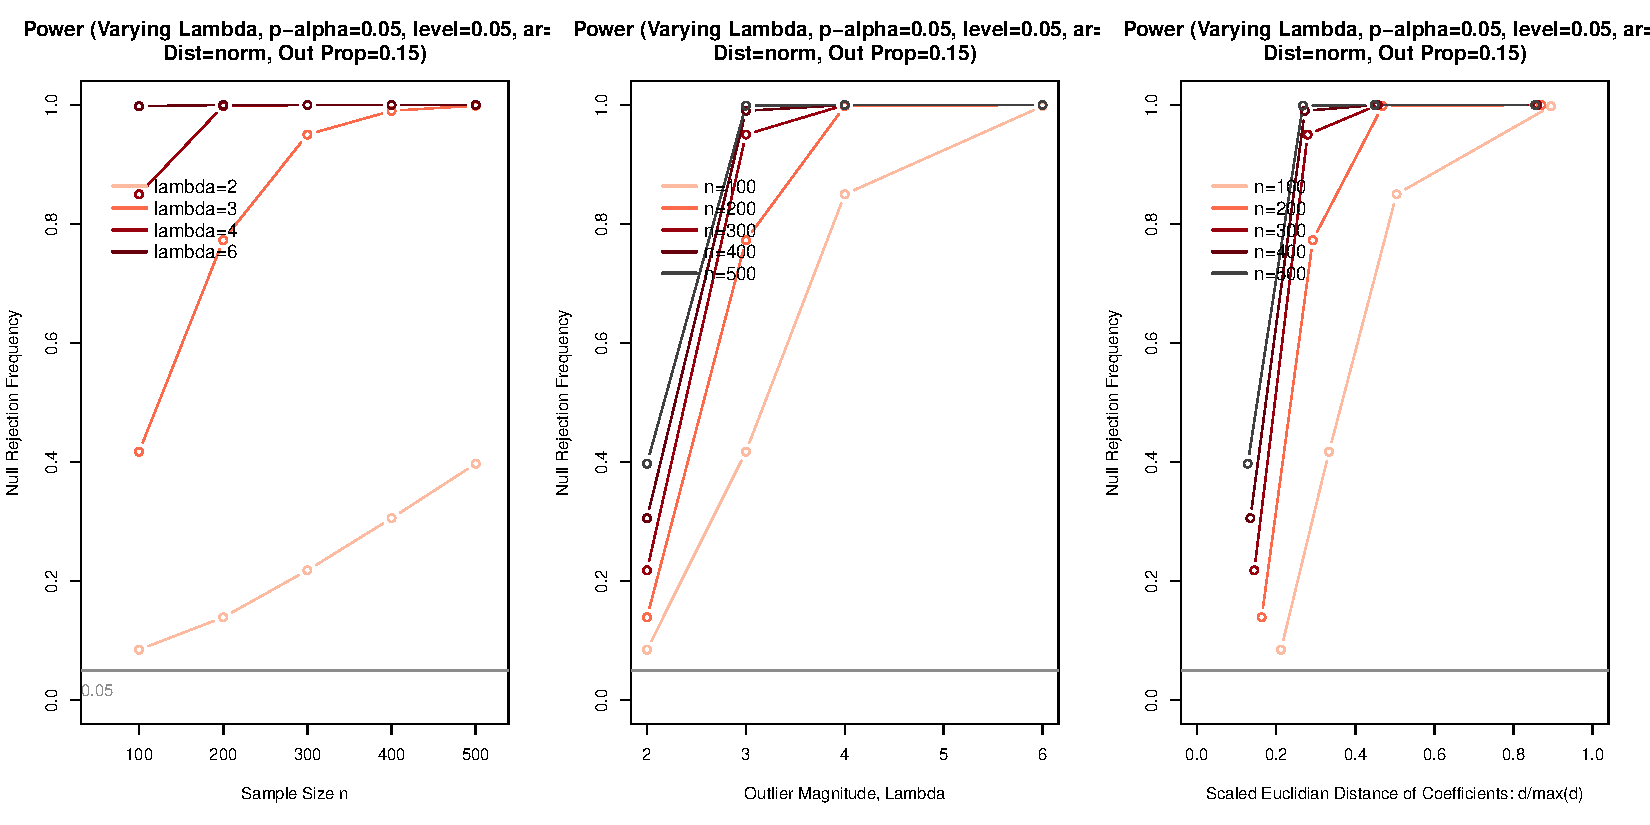
\includegraphics[width = \textwidth]{alt_ar0_nreg5_palpha0.05_distnorm_outprop0.15.pdf}
\caption{Simulation performance under the alternative for varying sample sizes and outlier magnitudes when the dependent variable exhibits no autocorrelation and 15\% of the sample is outlier-contaminated.}
\label{fig_out_sim_alt15}
\end{figure}



\begin{figure}[!htbp]  %\vspace{-.35in}
\centering
%\includegraphics[scale=0.6]{{alt_ar0_nreg1_palpha0.05_distnorm_outprop0.1}.pdf}
\includegraphics[width = \textwidth]{{alt_ar0_nreg1_palpha0.05_distnorm_outprop0.1}.pdf}
\caption{Simulation performance under the alternative, testing a single regressor, for varying sample sizes and outlier magnitudes when the dependent variable exhibits no autocorrelation and 10\% of the sample is outlier-contaminated.}
\label{fig_out_sim_alt1_1reg}
\end{figure}



\begin{figure}[!htbp]  %\vspace{-.35in}
\centering
%\includegraphics[scale=0.6]{{alt_ar0.5_nreg5_palpha0.05_distnorm_outprop0.1}.pdf}
\includegraphics[width = \textwidth]{{alt_ar0.5_nreg5_palpha0.05_distnorm_outprop0.1}.pdf}
\caption{Simulation performance under the alternative for varying sample sizes and outlier magnitudes when the dependent variable exhibits some autocorrelation (AR coefficient = 0.5) and 10\% of the sample is outlier-contaminated.}
\label{fig_out_sim_alt1_5reg05}
\end{figure}



\begin{figure}[!htbp]  %\vspace{-.35in}
\centering
%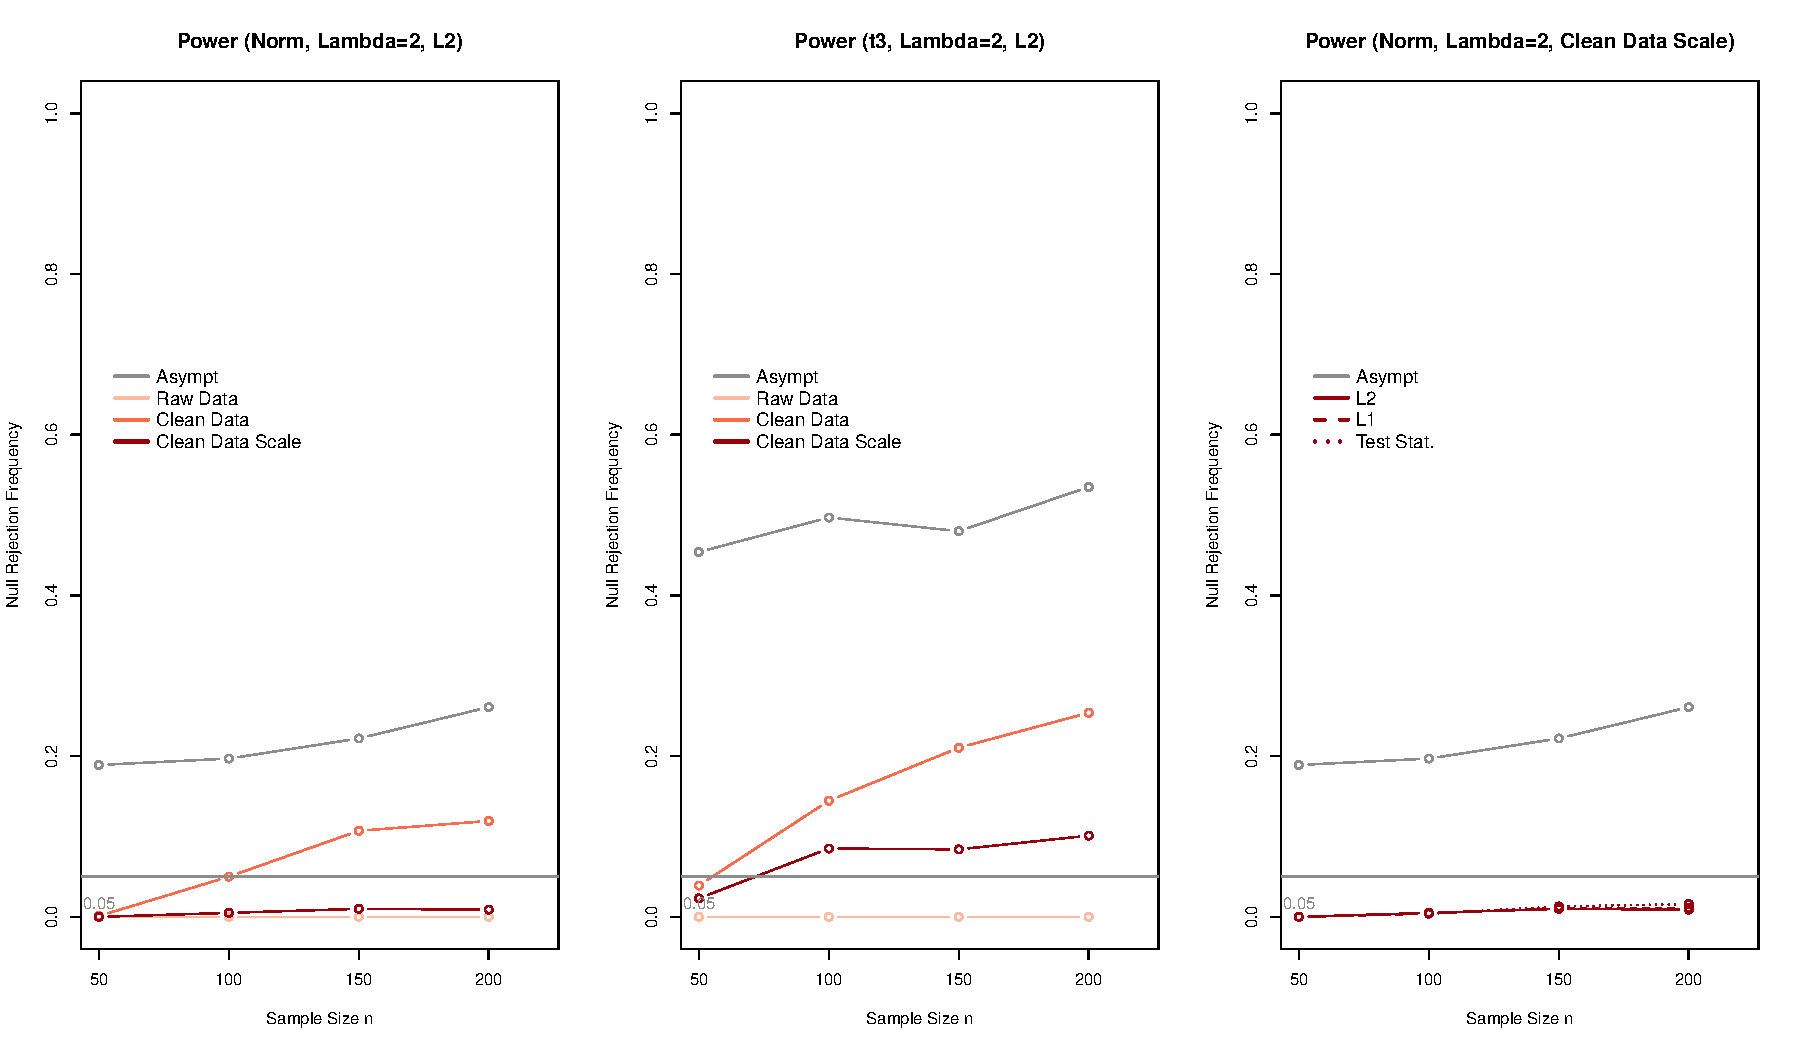
\includegraphics[scale=0.5]{boot_alt_lambda2.pdf}
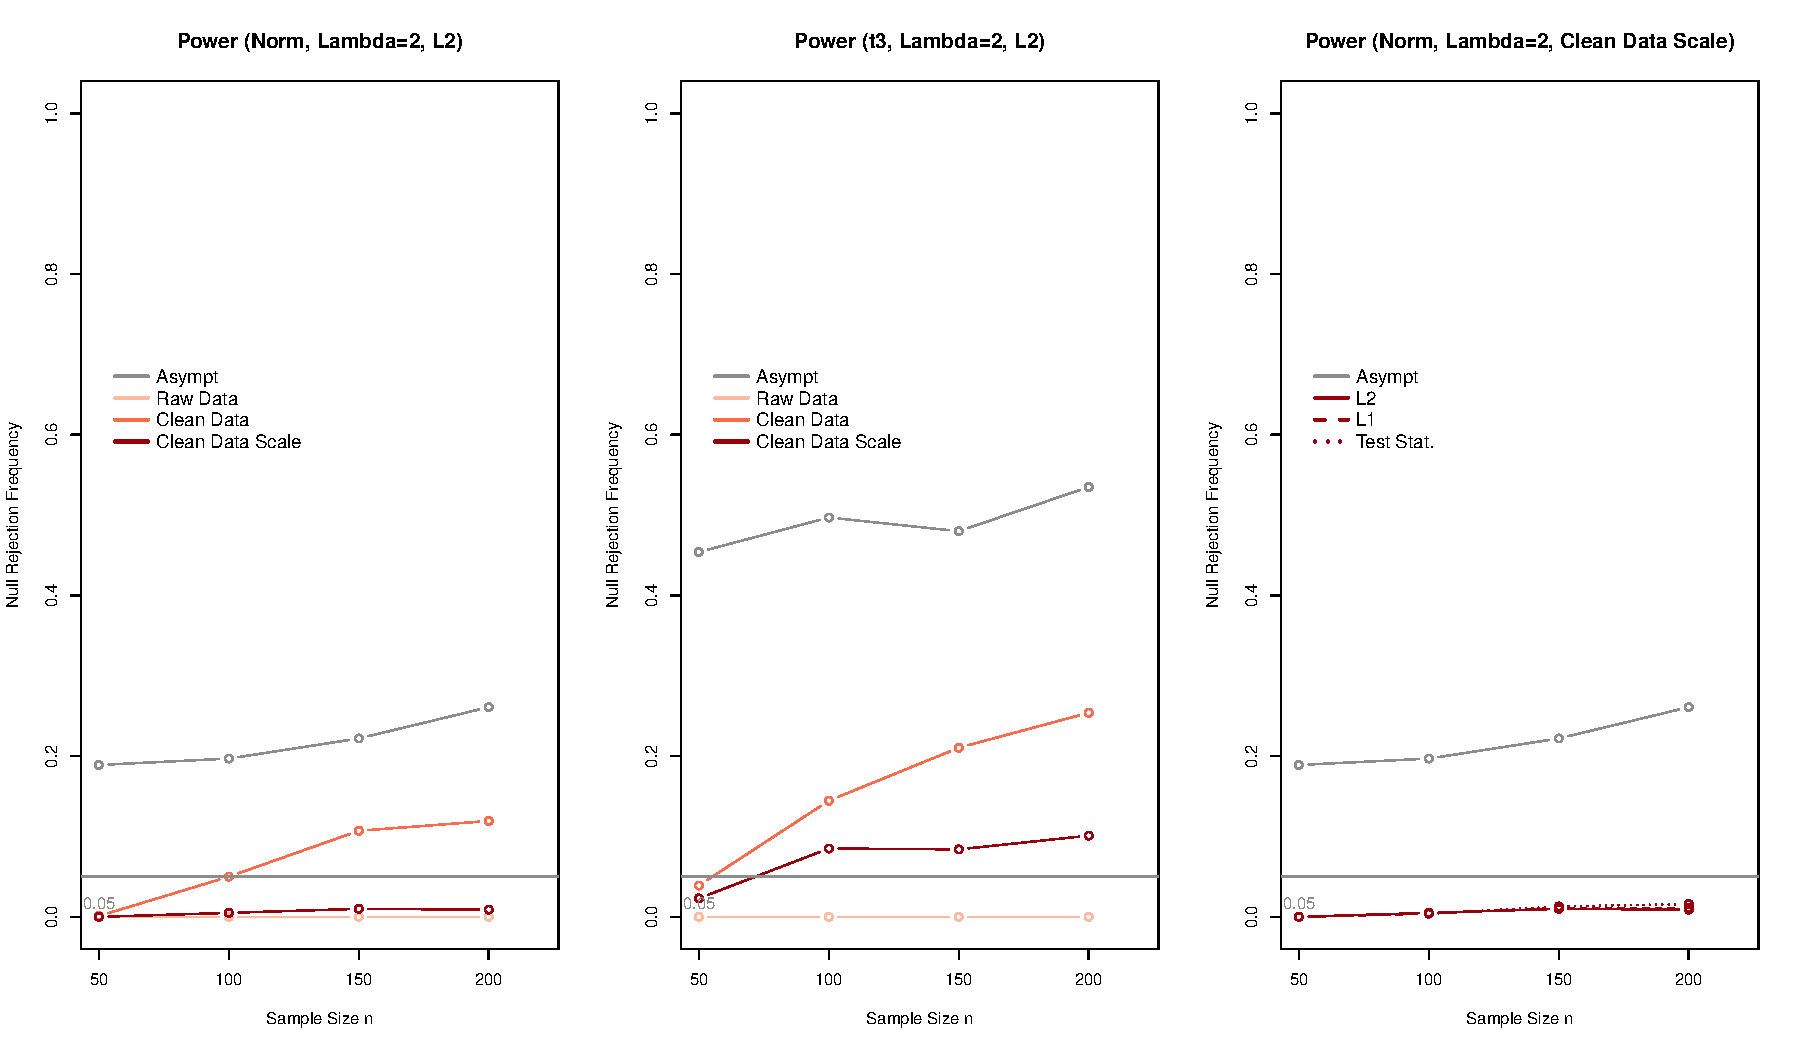
\includegraphics[width = \textwidth]{boot_alt_lambda2.pdf}
\caption{Simulation performance under the alternative for varying sample sizes when using the bootstrap implementations of our test (for outlier magnitude of 2SD of the error term).}
\label{fig_out_sim_alt_boot2}
\end{figure}

\begin{figure}[!htbp]  %\vspace{-.35in}
\centering
%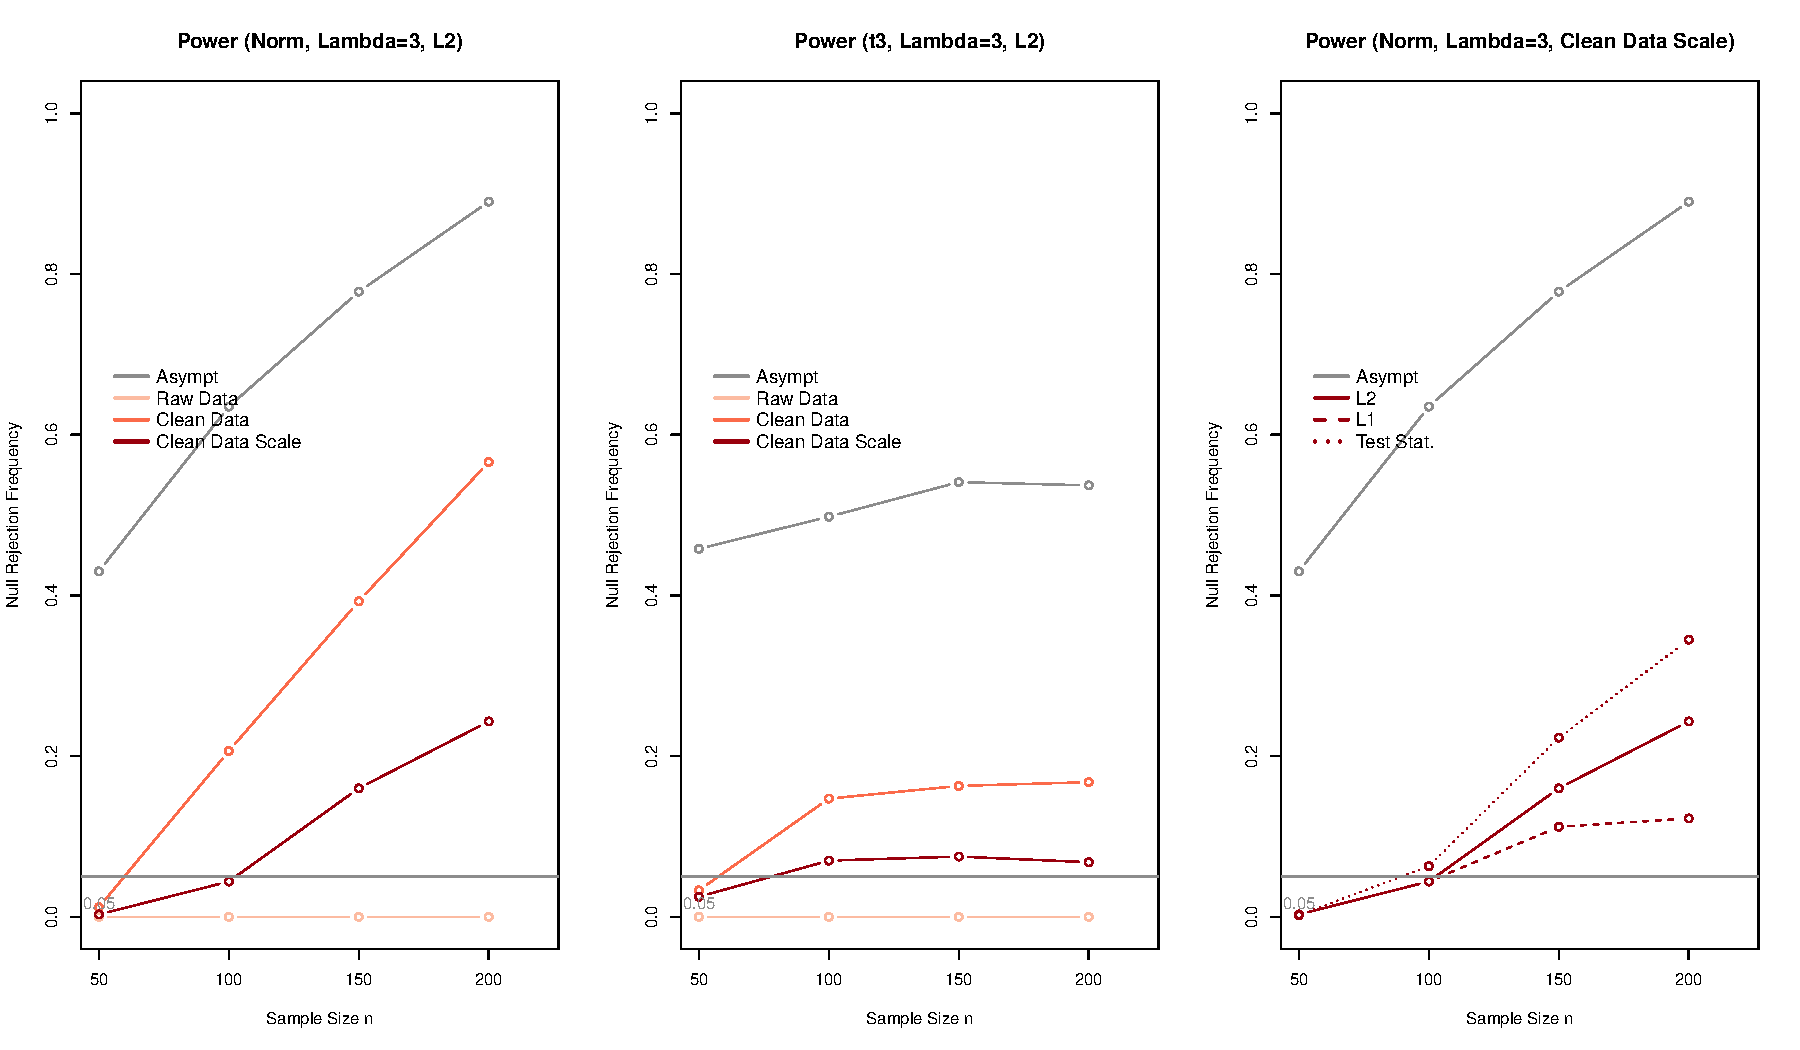
\includegraphics[scale=0.5]{boot_alt_lambda3.pdf}
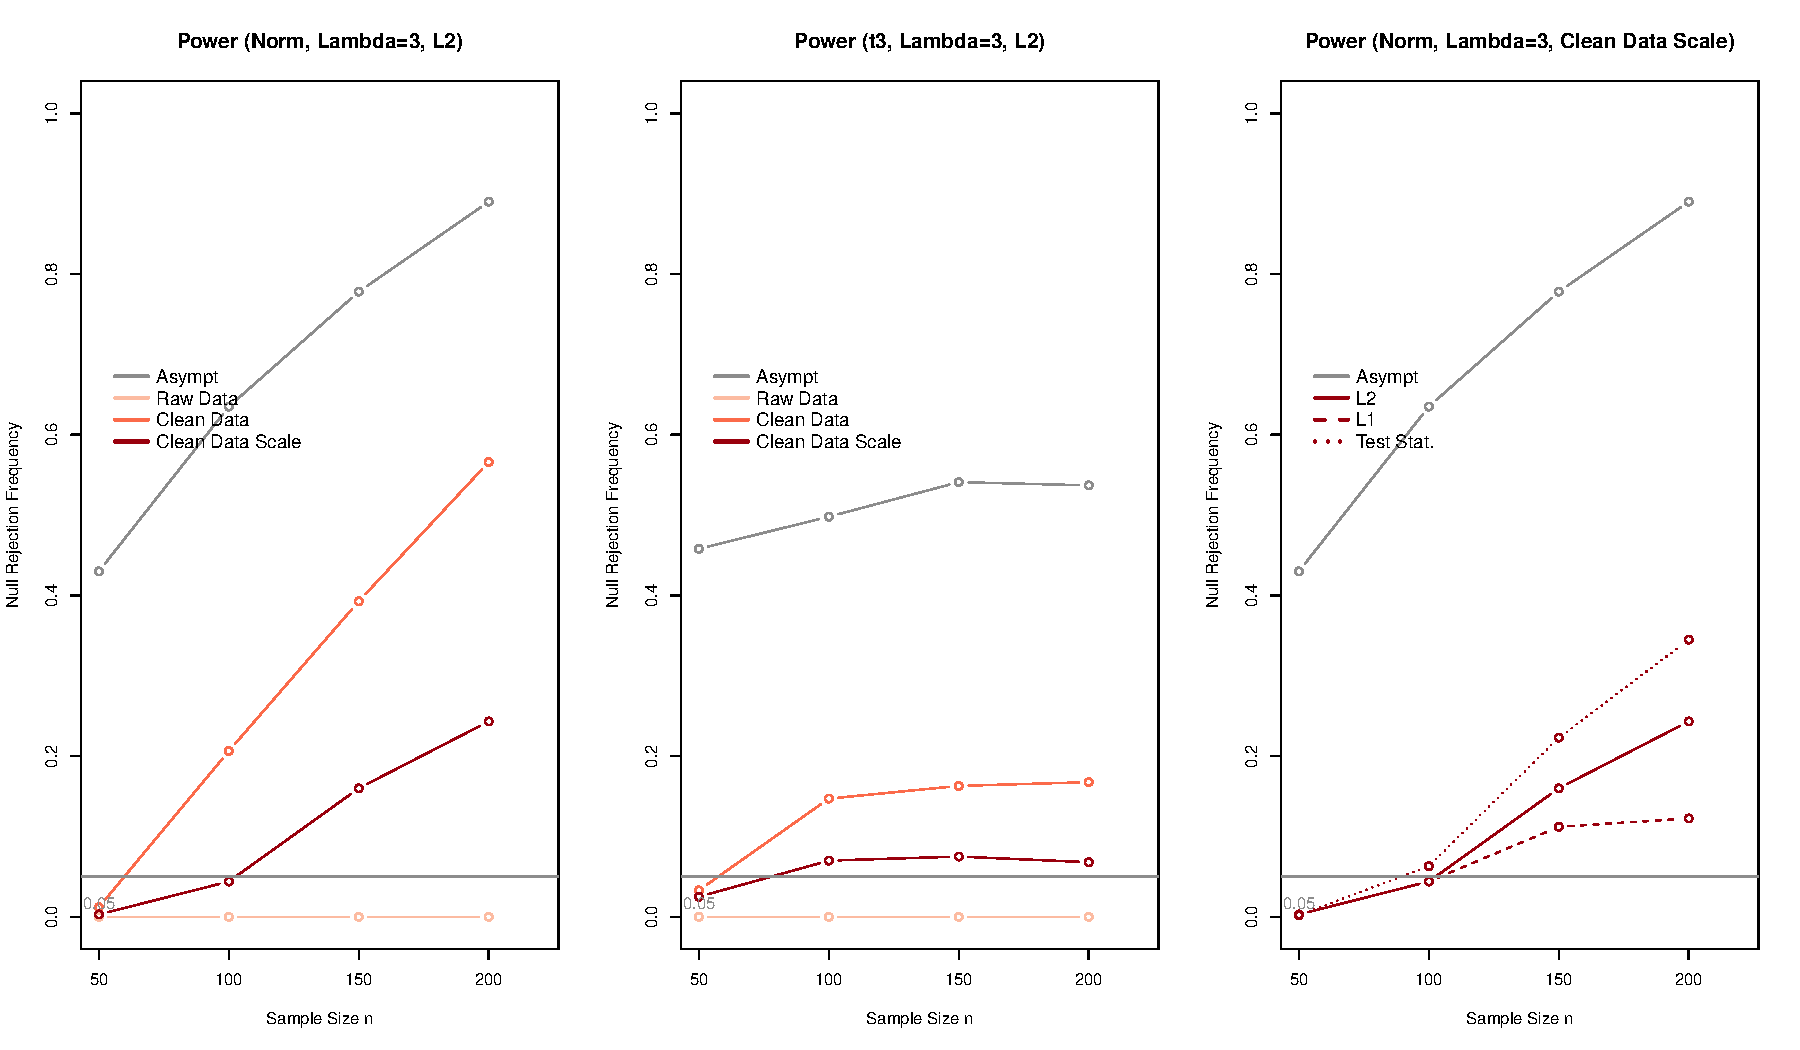
\includegraphics[width = \textwidth]{boot_alt_lambda3.pdf}
\caption{Simulation performance under the alternative for varying sample sizes when using the bootstrap implementations of our test (for outlier magnitude of 3SD of the error term).}
\label{fig_out_sim_alt_boot3}
\end{figure}

%\subsection{Simulation Results presented in Tables}


%\begin{table}
                   \caption{Simulation performance under the alternative for varying sample sizes and outlier magnitudes when the dependent variable exhibits no autocorrelation and 15% of the sample is outlier-contaminated.}
                   \label{simulation_table_appendix_1}
\centering
\begin{tabular}{rrrrrr}
\toprule
\multicolumn{2}{c}{ } & \multicolumn{2}{c}{Normal Distr.} & \multicolumn{2}{c}{$t_3$ Distr.} \\
\cmidrule(l{3pt}r{3pt}){3-4} \cmidrule(l{3pt}r{3pt}){5-6}
\multicolumn{2}{c}{ } & \multicolumn{4}{c}{$\gamma$} \\
\cmidrule(l{3pt}r{3pt}){3-6}
n & \# Regressors & 0.01 & 0.05 & 0.01 & 0.05\\
\midrule
\addlinespace[0.3em]
\multicolumn{6}{l}{\textbf{Level 0.01}}\\
\hspace{1em}100 & 5 & 0.107 & 0.757 & 0.029 & 0.393\\
\hspace{1em}200 & 5 & 0.056 & 0.809 & 0.018 & 0.433\\
\hspace{1em}300 & 5 & 0.044 & 0.844 & 0.017 & 0.452\\
\hspace{1em}400 & 5 & 0.034 & 0.856 & 0.014 & 0.463\\
\hspace{1em}500 & 5 & 0.031 & 0.868 & 0.015 & 0.469\\
\addlinespace[0.3em]
\multicolumn{6}{l}{\textbf{Level 0.05}}\\
\hspace{1em}100 & 5 & 0.194 & 0.840 & 0.088 & 0.548\\
\hspace{1em}200 & 5 & 0.123 & 0.886 & 0.069 & 0.594\\
\hspace{1em}300 & 5 & 0.103 & 0.910 & 0.063 & 0.613\\
\hspace{1em}400 & 5 & 0.092 & 0.919 & 0.060 & 0.631\\
\hspace{1em}500 & 5 & 0.084 & 0.927 & 0.060 & 0.635\\
\bottomrule
\end{tabular}
\end{table}


\clearpage
\section{Additional Projection Results} \label{sec_add_proj}

To alleviate concerns of endogeneity between $\Delta log(y)_{i,t}$ and $log(y)_{i, t}$, we also present a model using $log(y)_{i, t-1}$ (see equation (\ref{pan_adapt.L1}) below).

\begin{small}
\begin{equation}
\label{pan_adapt.L1}
\Delta log(y)_{i,t} = \alpha_i + \lambda_t + \beta_1 T_{i,t} + \beta_2 T^2_{i,t} + \beta_3 \left[ T_{i,t} \times  log(y)_{i, t-1} \right] + \beta_4 \left[  T^2_{i,t} \times  log(y)_{i, t-1} \right] + x_{i,t}'\gamma + u_{i,t}
\end{equation}
\end{small}



\begin{figure}[!htbp]  %\vspace{-.35in}
\centering
%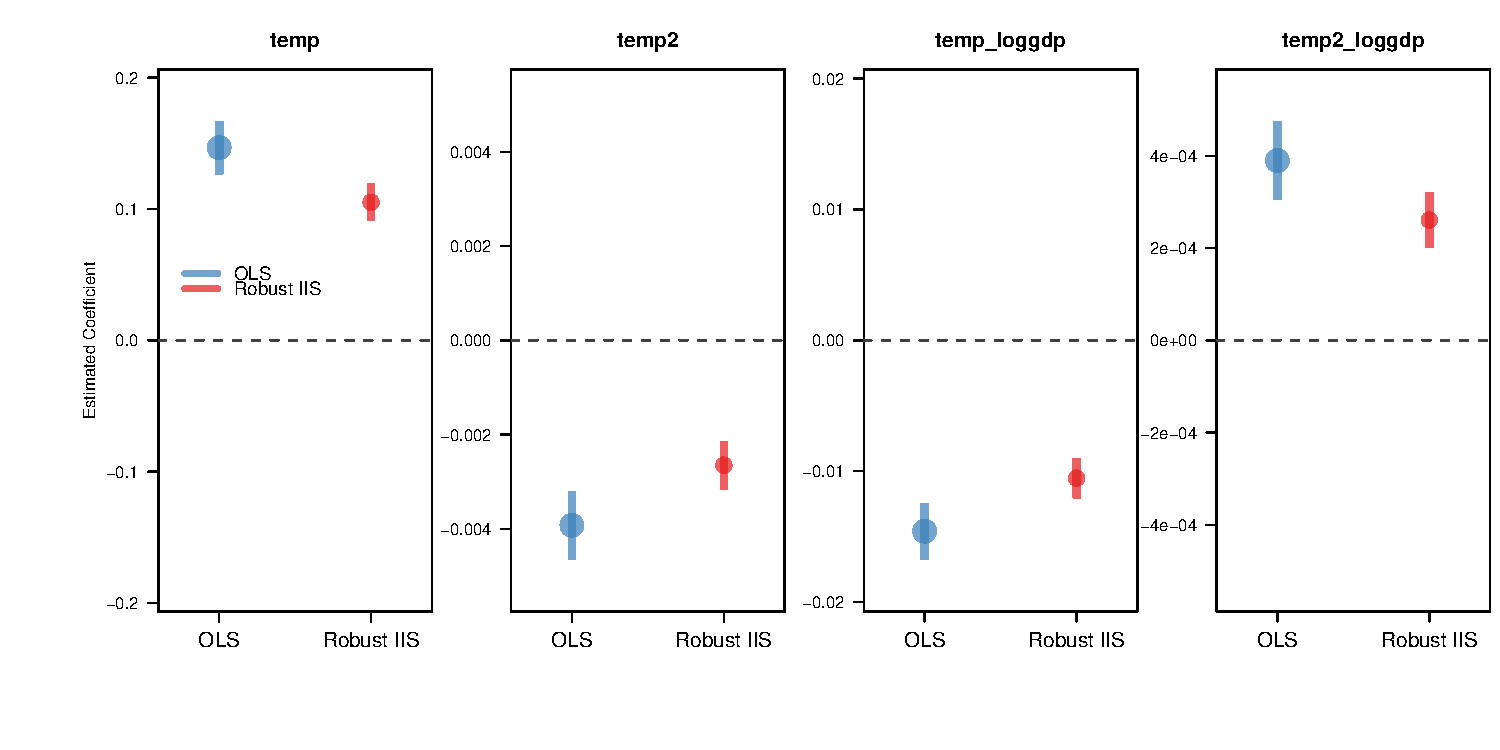
\includegraphics[scale=0.65]{coef_v2_lag.pdf}
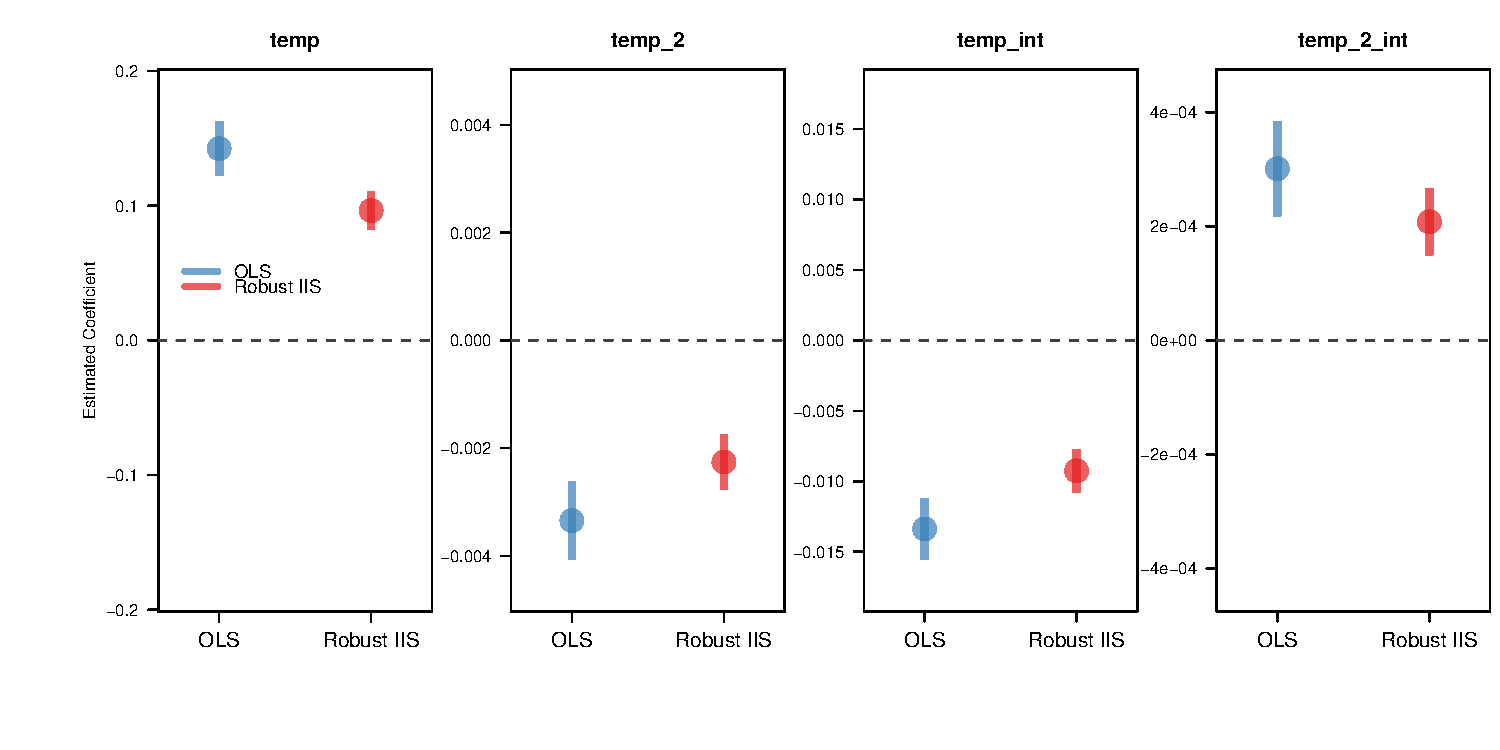
\includegraphics[width = \textwidth]{coef.adapt.L1.pdf}
\caption{Projection with Lagged GDP per capita. Estimated Impact of Temperatures on GDP Per Capita Growth Allowing for Adaptation and Controlling for Outliers. Coefficients on temperatures and the income interaction terms are shown using OLS and the robust IIS estimator. Note that scale of the y-axis differs across plots.}
\label{fig_dist_coef_app1_appendix}
\end{figure}

\begin{figure}[!htbp]  %\vspace{-.35in}
\centering
%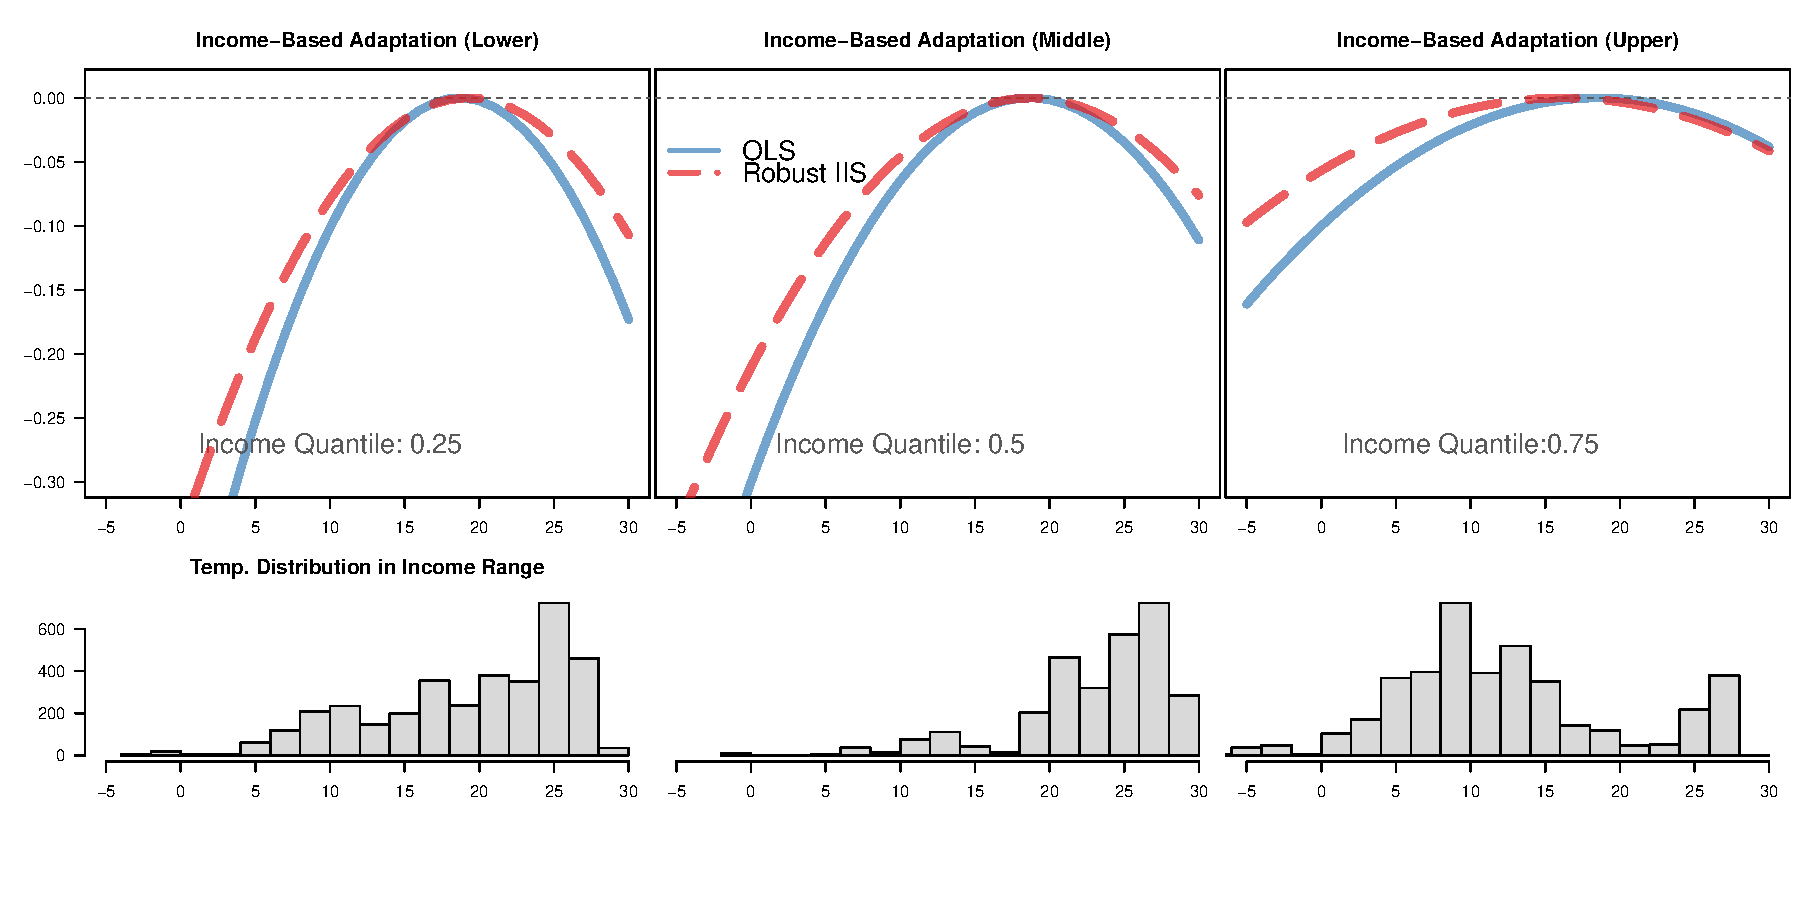
\includegraphics[scale=0.55]{eff_v1_lag.pdf}
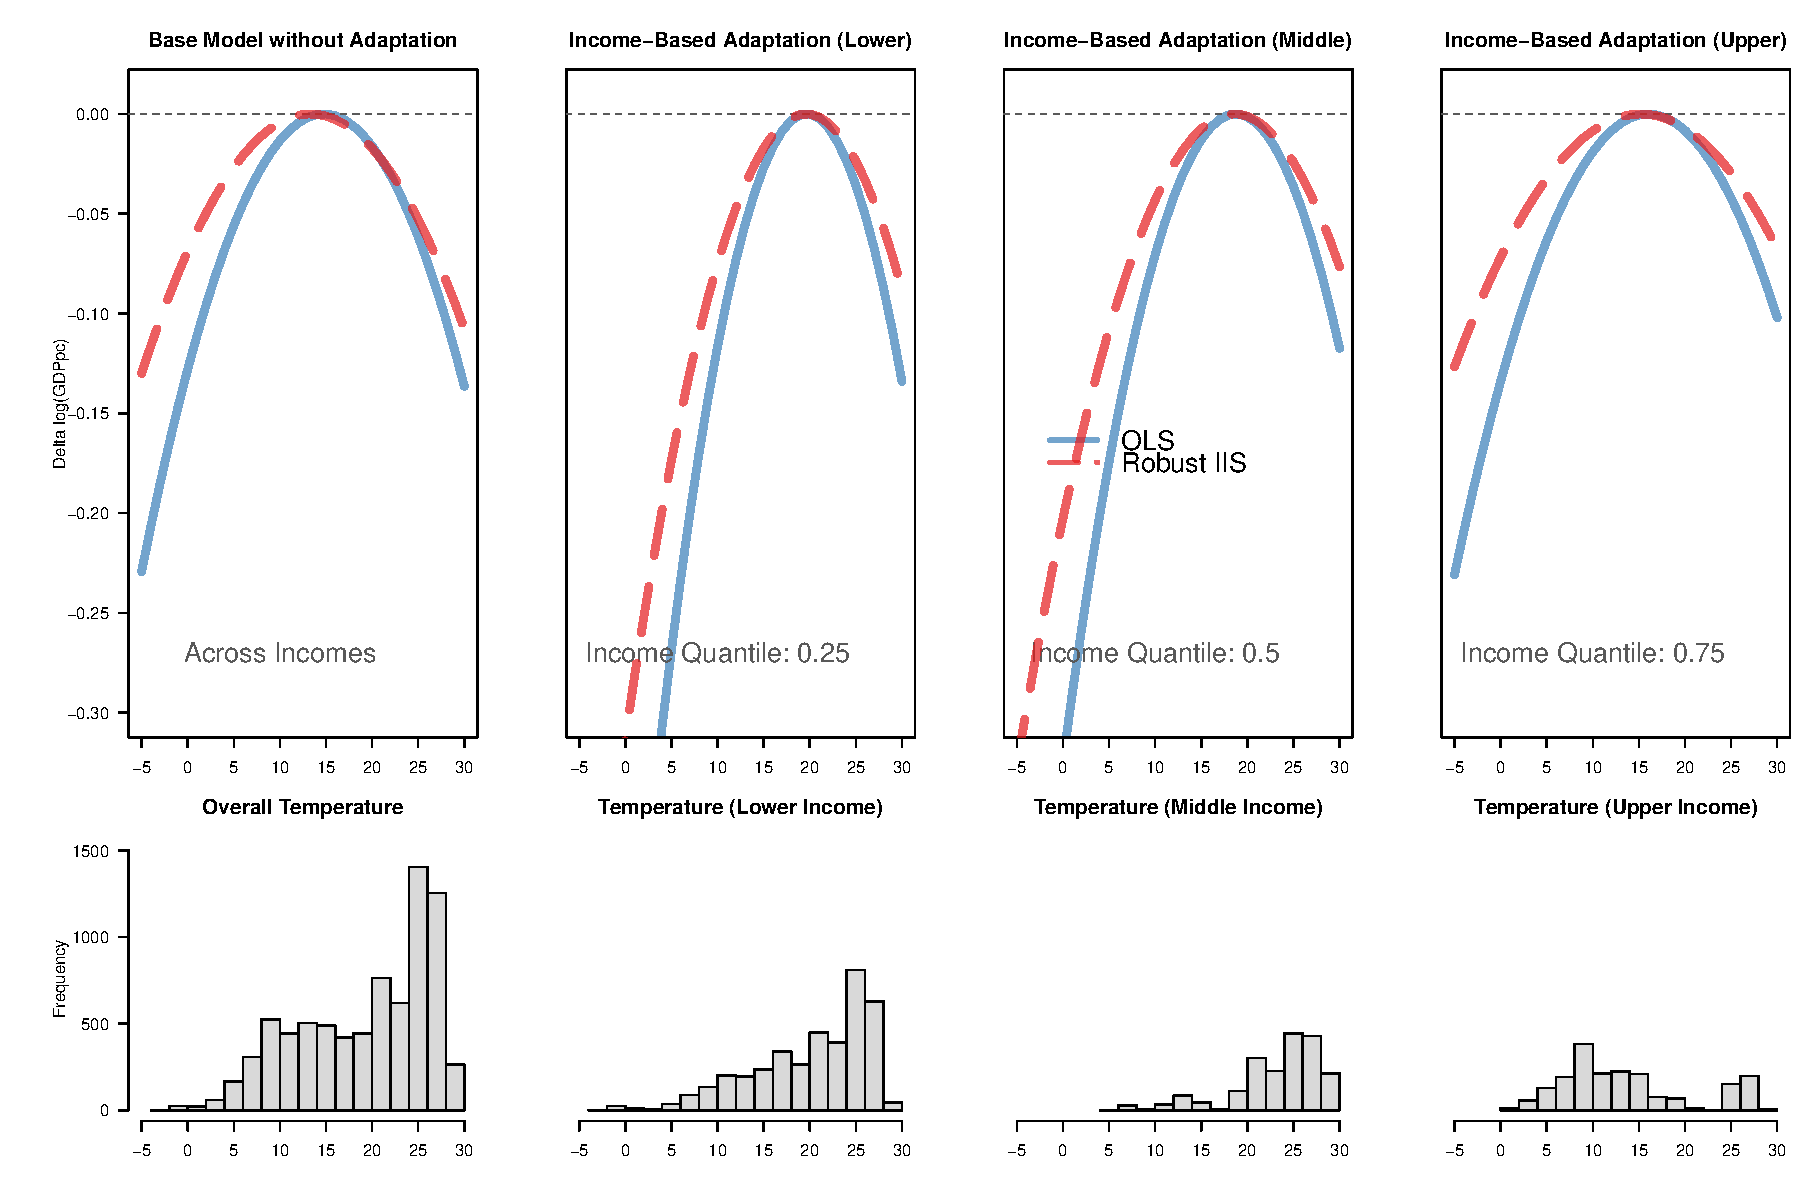
\includegraphics[width = \textwidth]{eff.adapt.L1.v2.pdf}
\caption{Projection with Lagged GDP per capita. Estimated Impact of Temperatures on GDP Per Capita Growth Allowing for Adaptation and Controlling for Outliers. OLS-estimated relationship shown in blue, robust IIS estimated relationship shown in red. Estimated non-linear impact function for different three different income levels (middle panels) and the observed country level temperatures (bottom panels): countries in at the 25\textsuperscript{th} income percentile, countries with median income, and countries at the 75\textsuperscript{th} income percentile. Observed temperatures across income ranges are shown in the lower panel. }
\label{fig_dist_app1_appendix}
\end{figure}



\begin{figure}[!htbp]  \vspace{-.35in}
\centering
%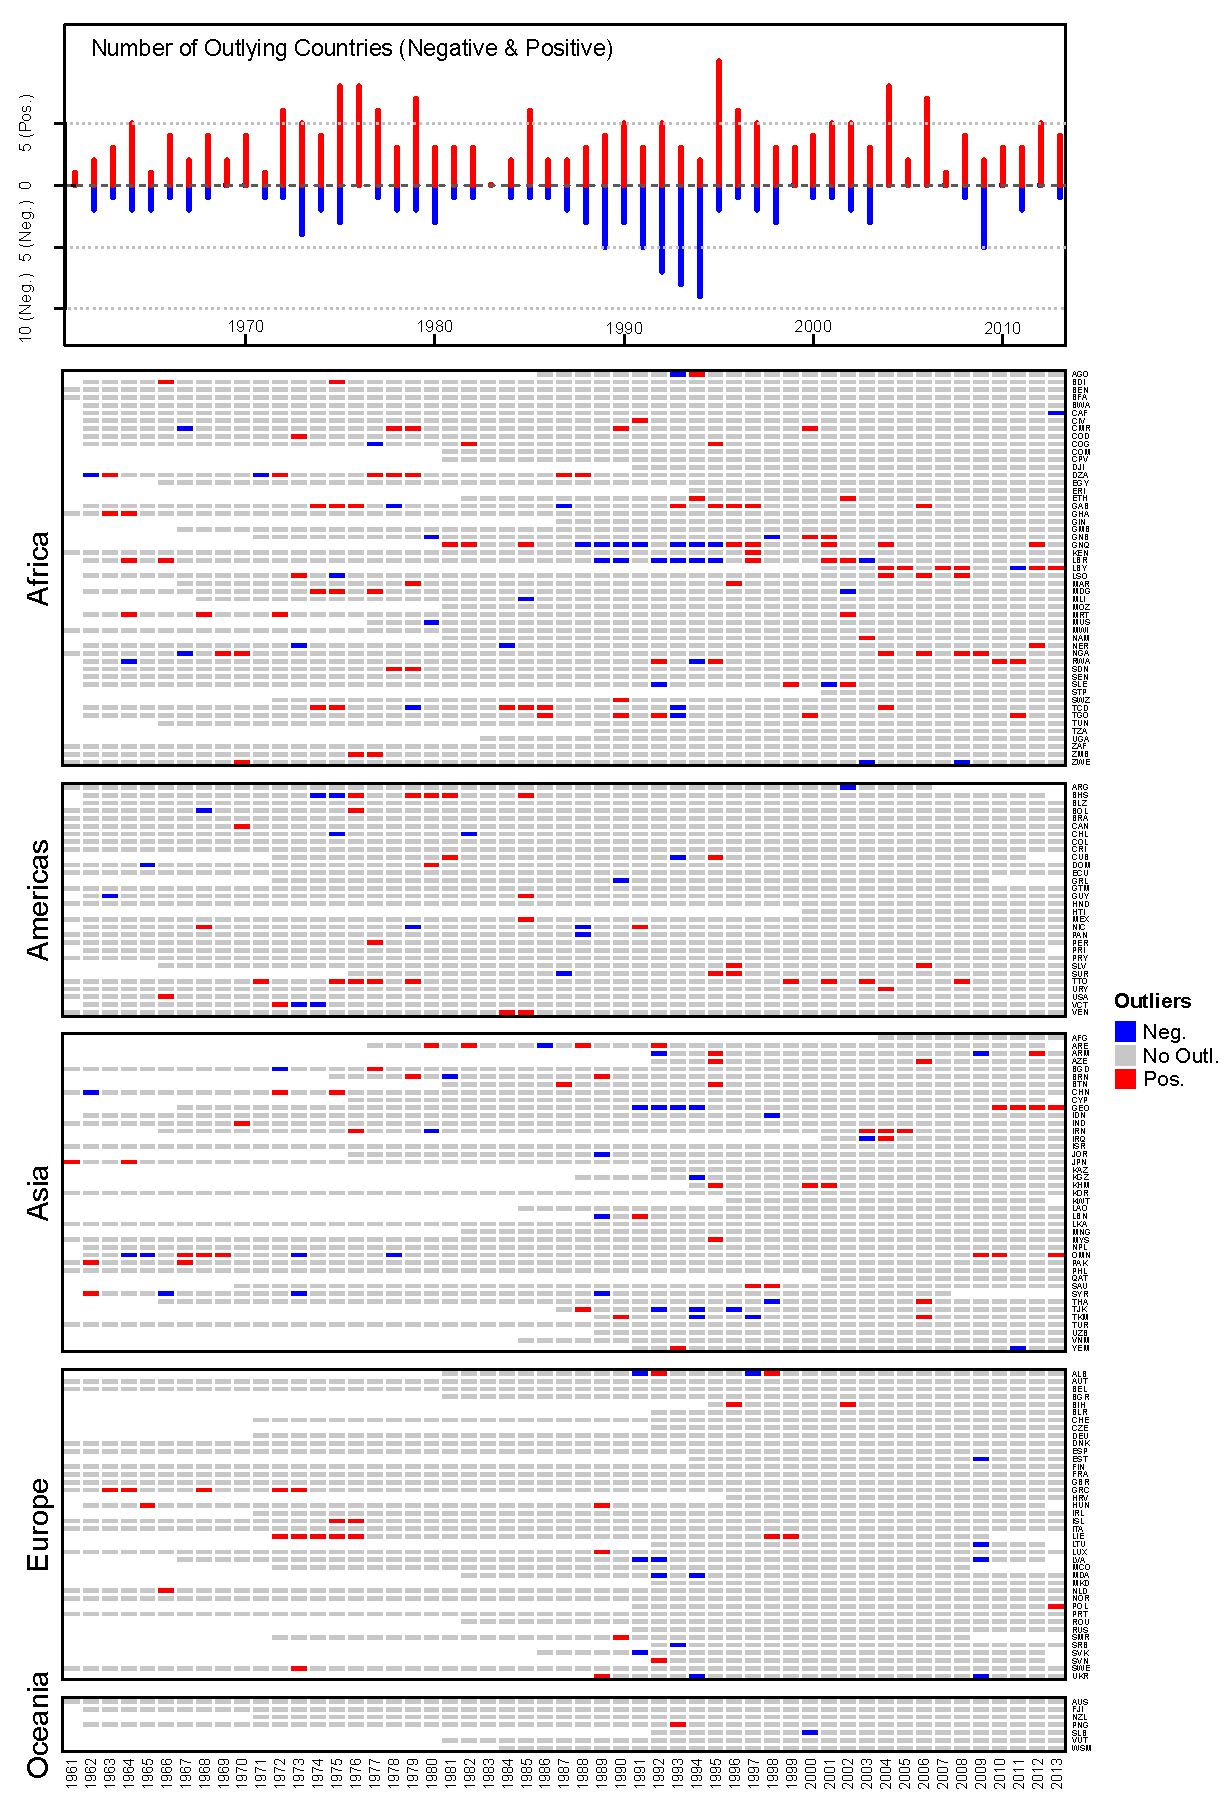
\includegraphics[scale=0.7]{heat1_lag_v1_edited.pdf}
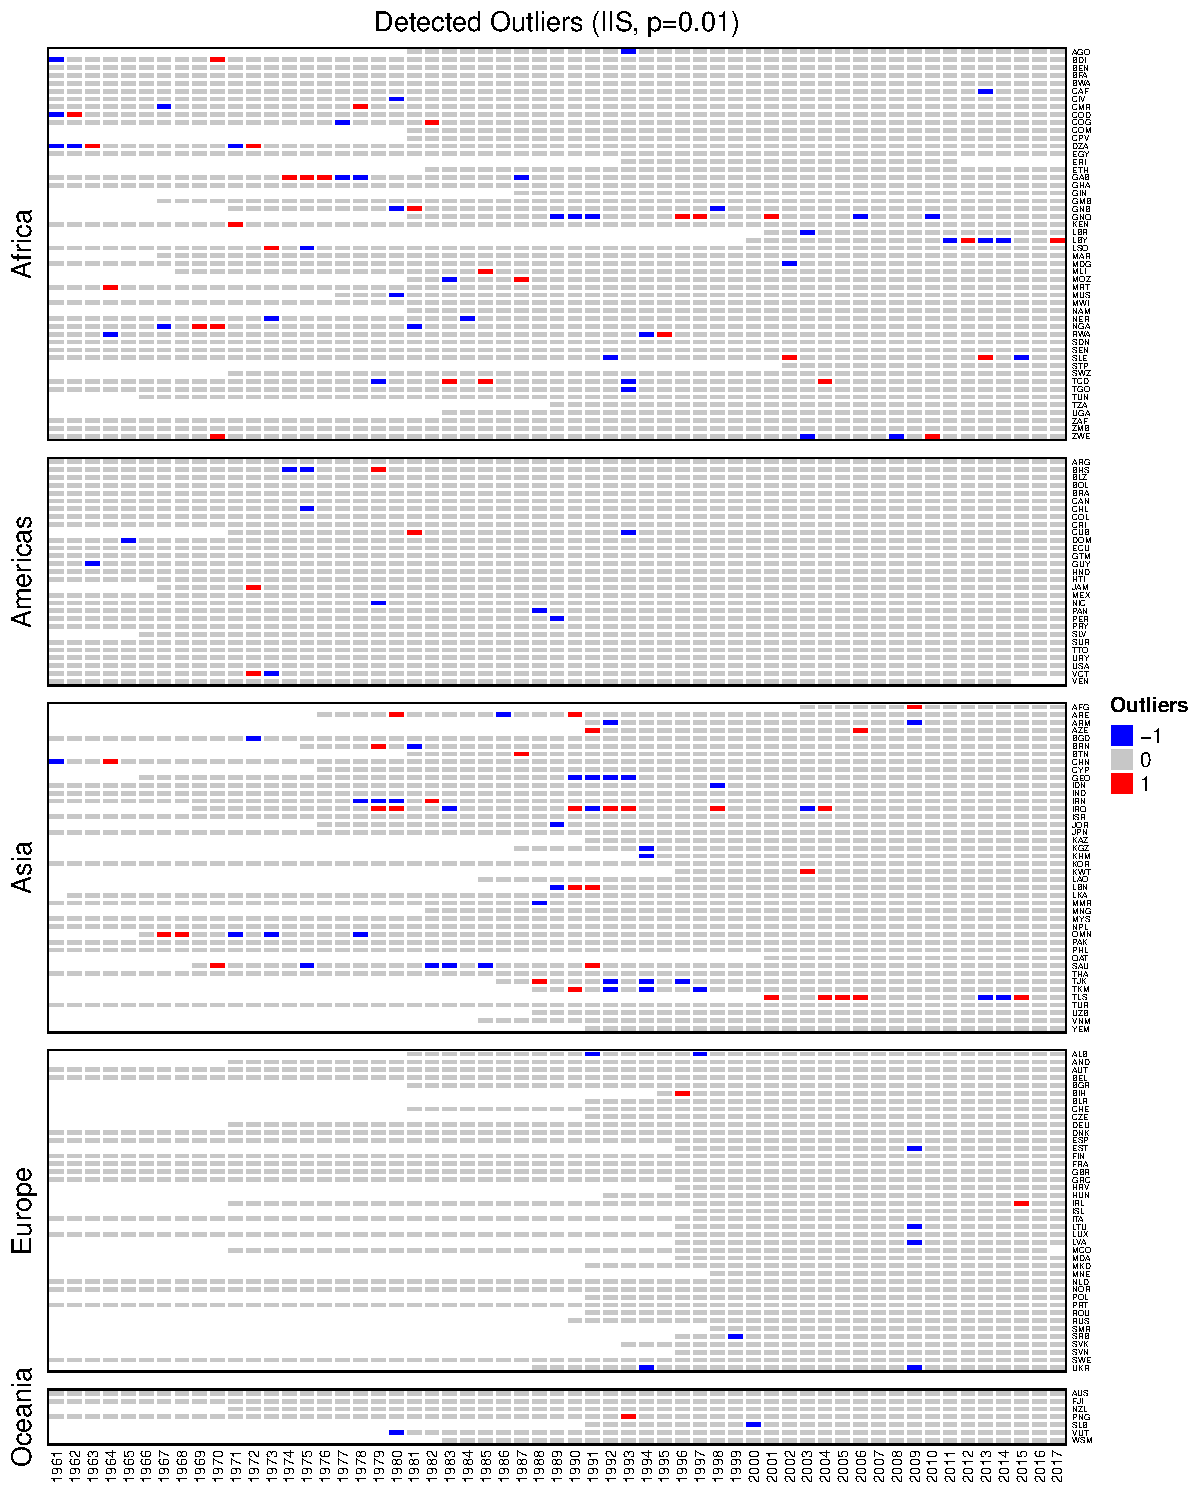
\includegraphics[width = \textwidth]{heat1.pdf}
\caption{Detected Outliers using the robust IIS estimator across countries and time in the global cross-country panel from 1961-2017 in the base model. Top Figure panel shows the number of positive (red) and negative (blue) outliers aggregated over countries in each year. Bottom panel shows country-year observations as gray when not outlying, blue when there is a negative outliers, and red for positive outliers.}
\label{fig_out_app1_appendix}
\end{figure}

\begin{figure}[!htbp]  \vspace{-.35in}
\centering
%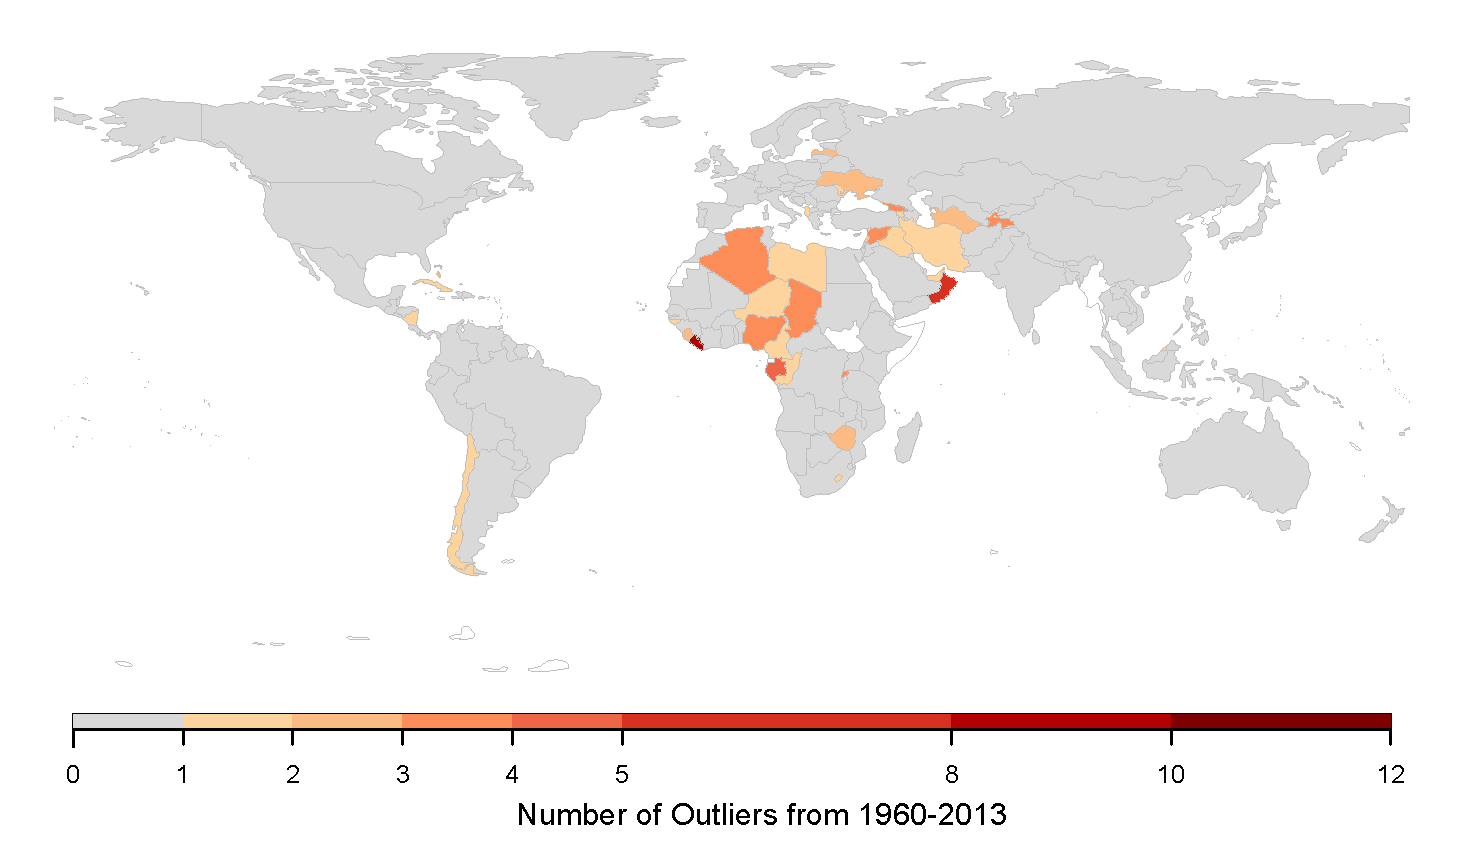
\includegraphics[scale=0.6]{ctry_map_lag_edited.pdf}
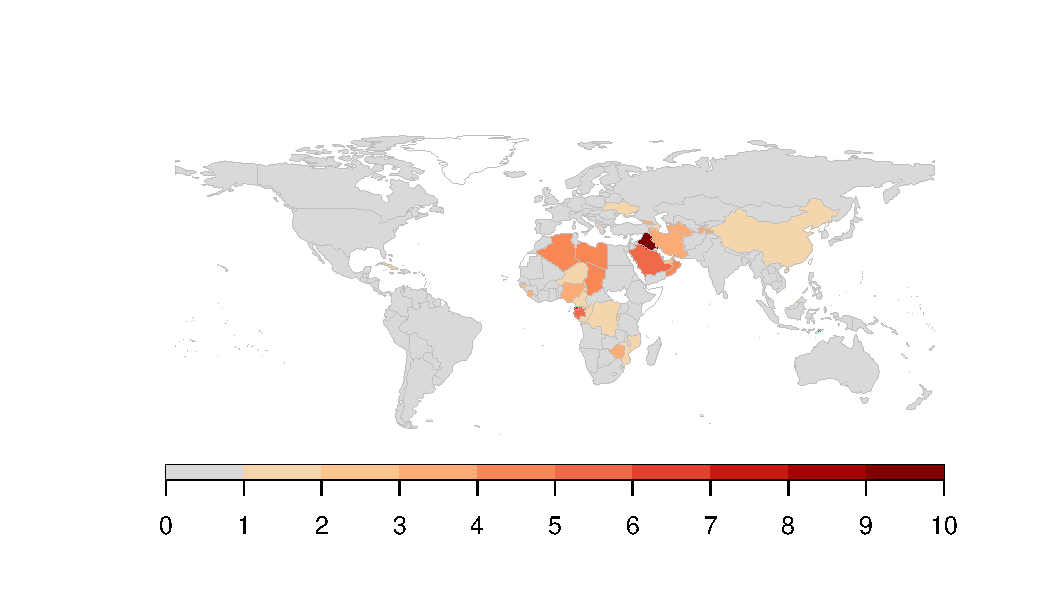
\includegraphics[width = \textwidth]{ctry_map.pdf}
\caption{Detected outliers aggregated over the full sample of 1961 - 2017 by country in the panel in the base model. Gray denotes no outliers detected. }
\label{fig_map_app1_appendix}
\end{figure}


\begin{figure}[!htbp]  \vspace{-.35in}
\centering
%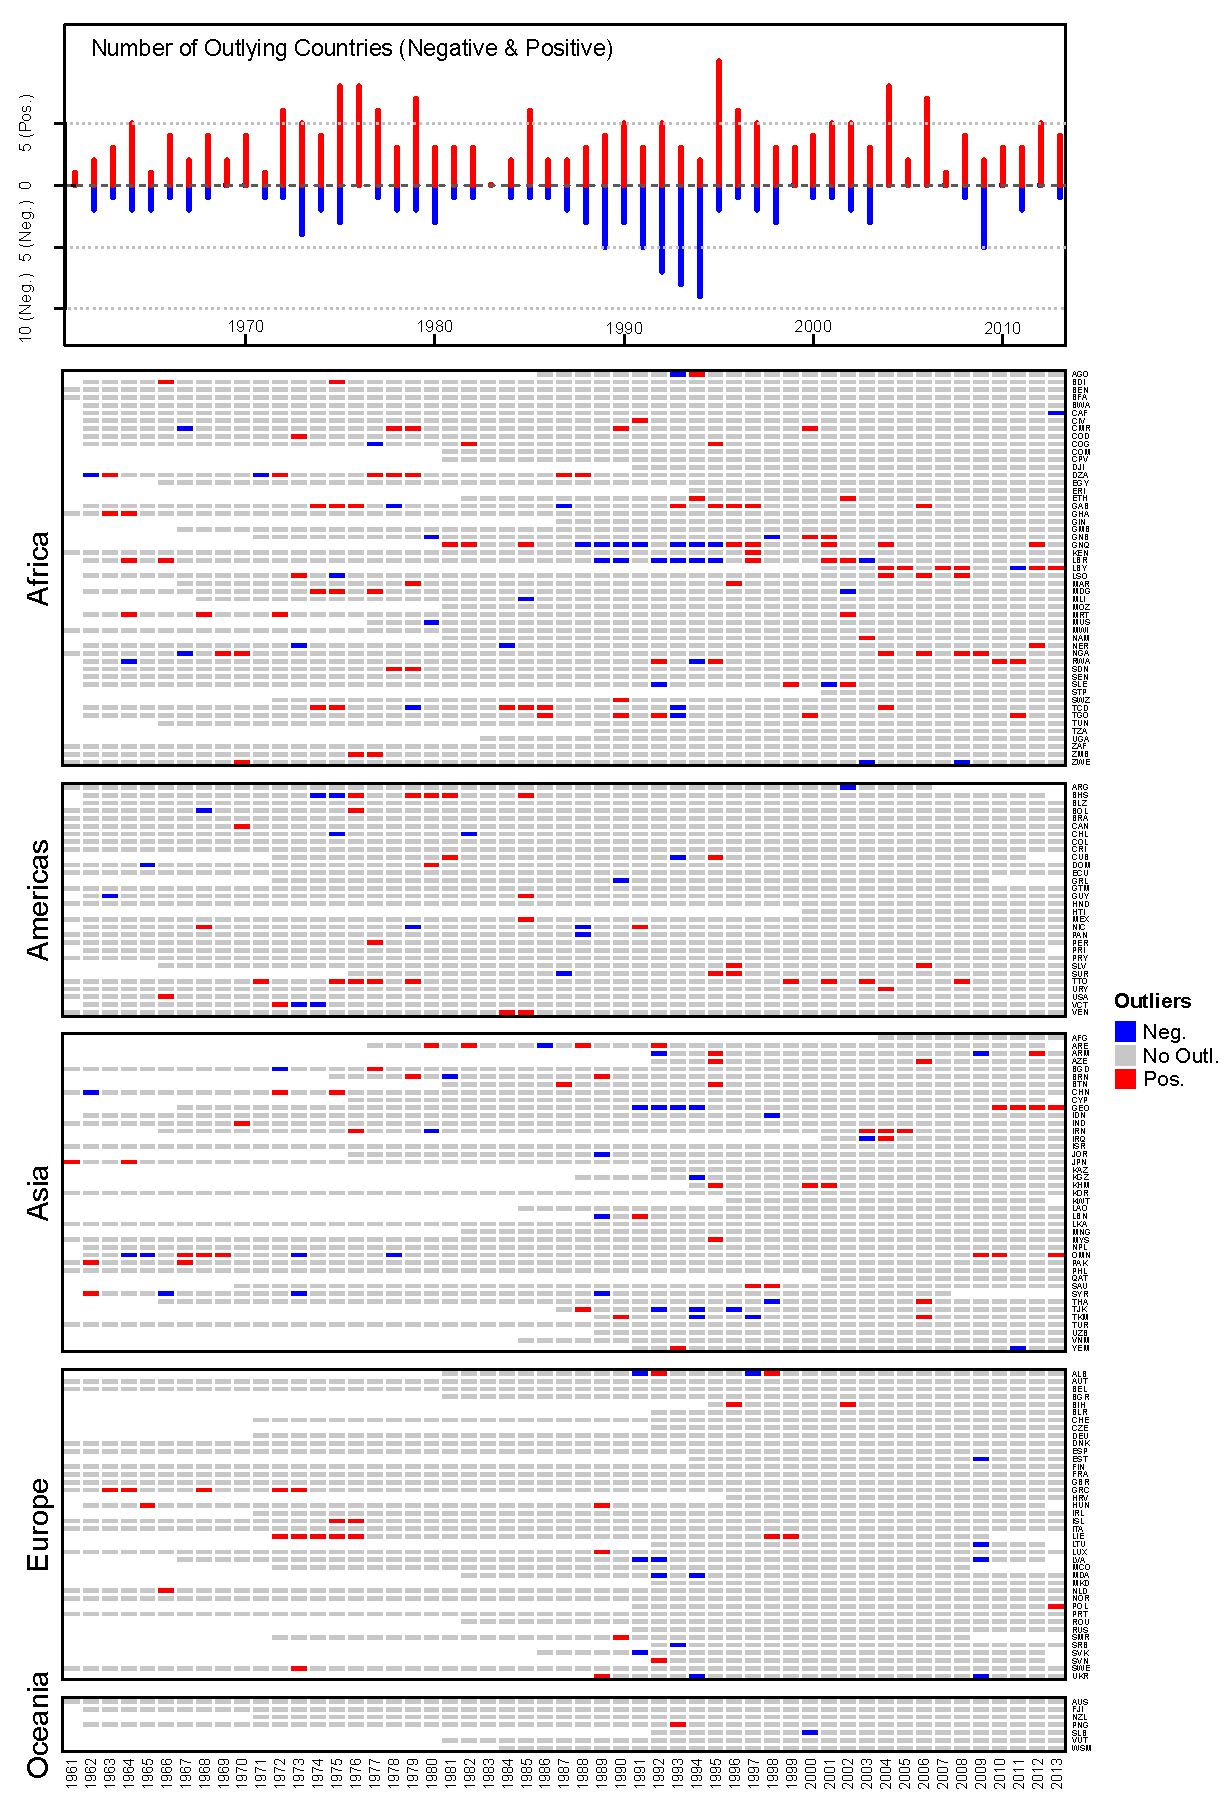
\includegraphics[scale=0.7]{heat1_lag_v1_edited.pdf}
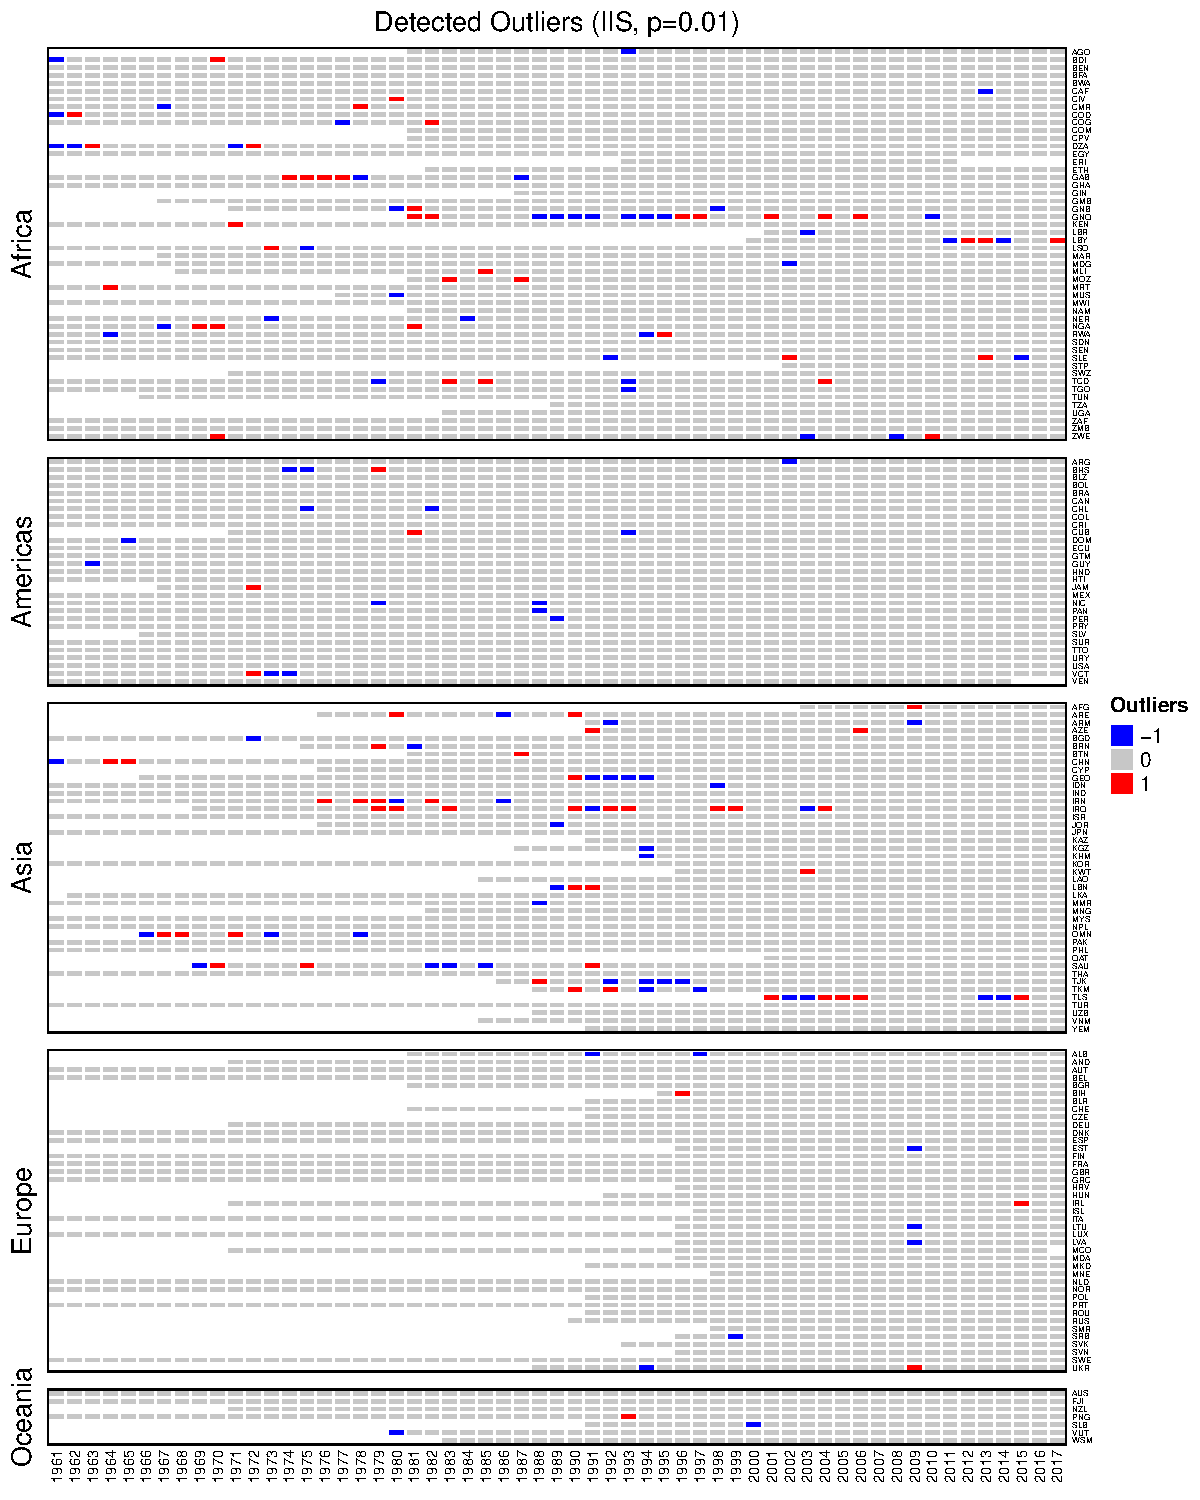
\includegraphics[width = \textwidth]{heat1_adapt.L1.pdf}
\caption{Detected Outliers using the robust IIS estimator across countries and time in the global cross-country panel from 1961-2017 in the adaptation model with lagged GDP per capita. Top Figure panel shows the number of positive (red) and negative (blue) outliers aggregated over countries in each year. Bottom panel shows country-year observations as gray when not outlying, blue when there is a negative outliers, and red for positive outliers.}
\label{fig_out_app2_appendix}
\end{figure}

\begin{figure}[!htbp]  \vspace{-.35in}
\centering
%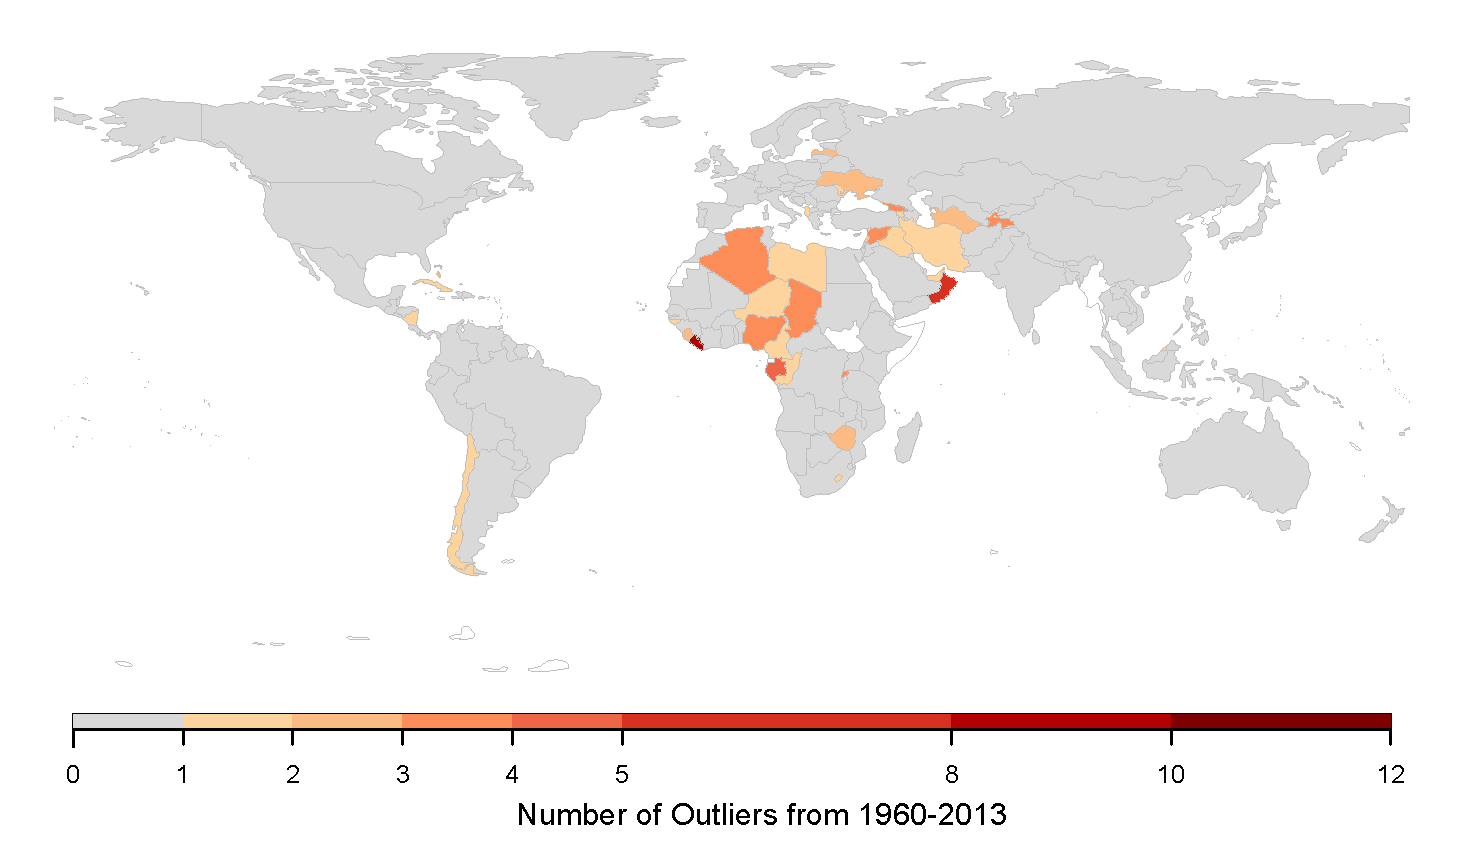
\includegraphics[scale=0.6]{ctry_map_lag_edited.pdf}
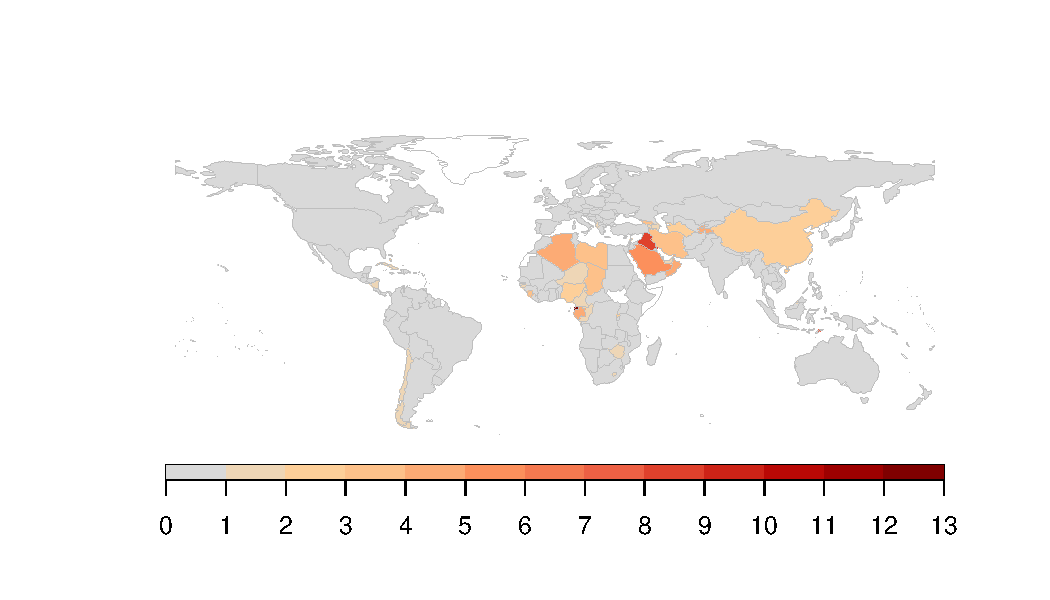
\includegraphics[width = \textwidth]{ctry_map_adapt.L1.pdf}
\caption{Detected outliers aggregated over the full sample of 1961 - 2017 by country in the panel in the adaptation model with lagged GDP per capita. Gray denotes no outliers detected.}
\label{fig_map_app2_appendix}
\end{figure}

\begin{figure}[!htbp]  \vspace{-.35in}
\centering
%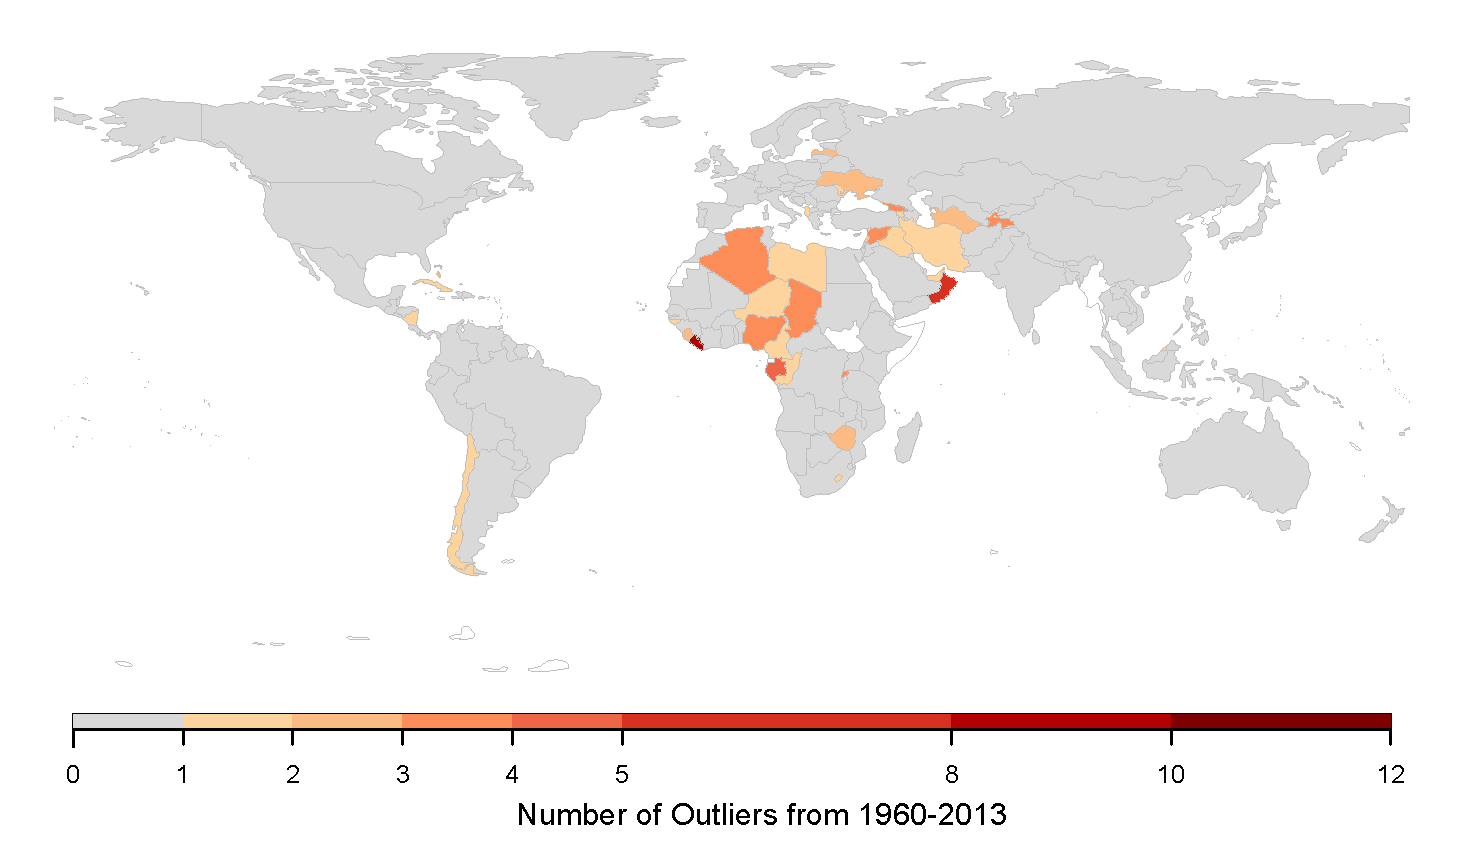
\includegraphics[scale=0.6]{ctry_map_lag_edited.pdf}
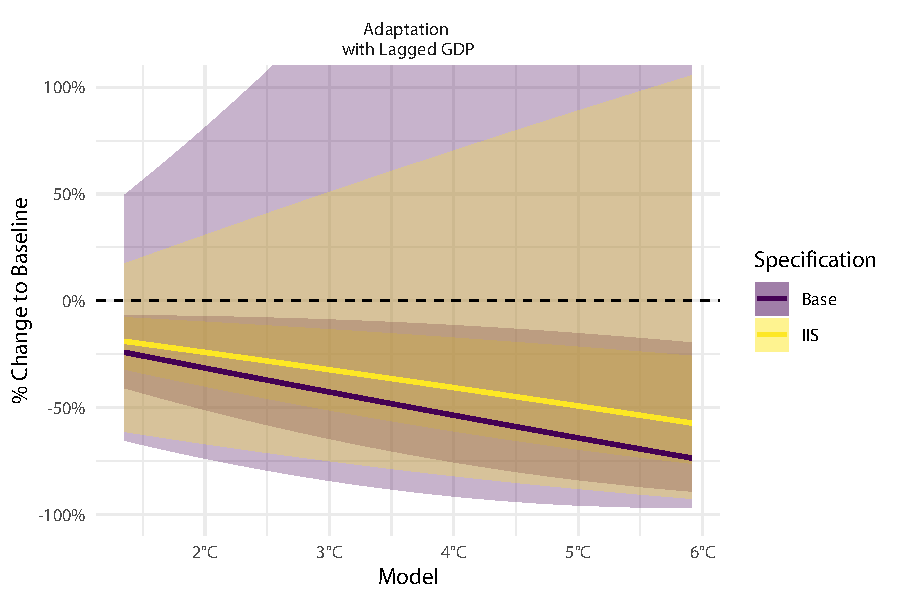
\includegraphics[width = \textwidth]{projections_noprcp_appendix.pdf}
\caption{Projected Damage Curve for the period 2090 - 2099. Projection excludes Precipitation Effect. Central line is the median. Shadings represent the interquartile range and a 90\% confidence interval.}
\label{fig_projection_lagged_noprcp}
\end{figure}

\begin{figure}[!htbp]  \vspace{-.35in}
\centering
%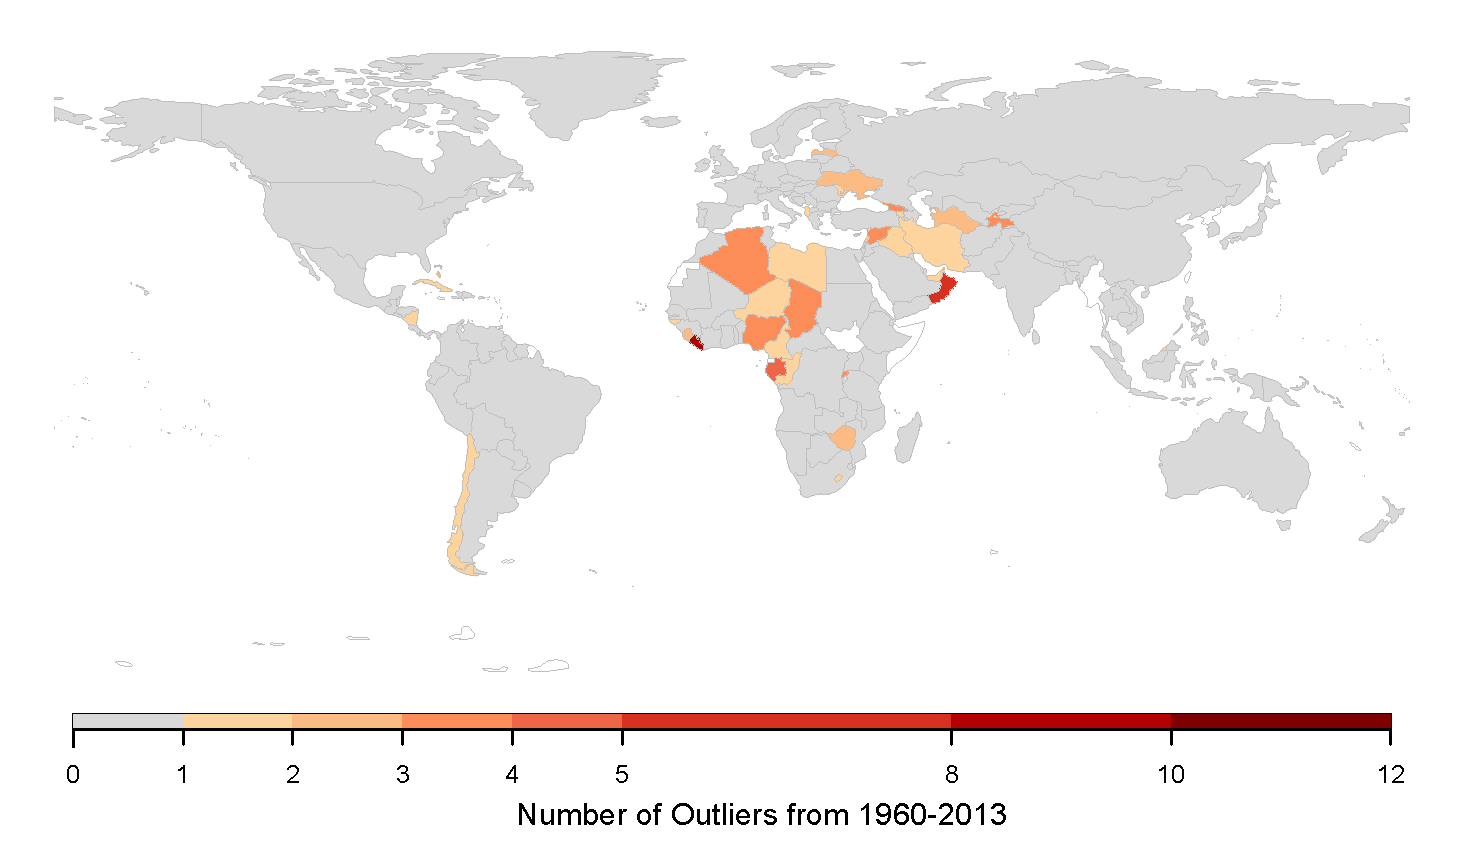
\includegraphics[scale=0.6]{ctry_map_lag_edited.pdf}
\includegraphics[width = \textwidth]{projections_withprcp_main.pdf}
\caption{Projected Damage Curve for the period 2090 - 2099. Projection includes Precipitation Effect.  Central line is the median. Shadings represent the interquartile range and a 90\% confidence interval.}
\label{fig_projection_base_withprcp}
\end{figure}


\begin{figure}[!htbp]  \vspace{-.35in}
\centering
%\includegraphics[scale=0.6]{ctry_map_lag_edited.pdf}
\includegraphics[width = \textwidth]{projections_withprcp_appendix.pdf}
\caption{Projected Damage Curve for the period 2090 - 2099. Projection includes Precipitation Effect.  Central line is the median. Shadings represent the interquartile range and a 90\% confidence interval.}
\label{fig_projection_lagged_withprcp}
\end{figure}


\begin{figure}[!htbp]  \vspace{-.35in}
\centering
%\includegraphics[scale=0.6]{ctry_map_lag_edited.pdf}
\includegraphics[width = \textwidth]{Map_IISBase_withprcp_diff.pdf}
\caption{Projected Climate Impacts for the period 2090 - 2099 and for all CMIP5 models with a mean warming above 4\textdegree C. Projection includes Precipitation Effect. Estimate shown is the median, grey indicates that the 90\% confidence interval spans 0.}
\label{fig_projection_map_withprcp}
\end{figure}




\end{document}

%%%%%%%%%%%%%%%%%%%%%%%%%%%%%%%%%%%%%%%%%%%%%%%%%%%%%

